
\documentclass[copyright,creativecommons]{eptcs} 
\providecommand{\event}{ICE 26} % Name of the event you are submitting to
\usepackage{underscore}           % Only needed if you use pdflatex.
 
\usepackage{breakurl}

\usepackage{wrapfig}

\usepackage{hyperref}
\usepackage{amsfonts}
\usepackage{amsmath}
\usepackage{amssymb}
\usepackage{amsthm}
\usepackage{amsbsy}
\usepackage{enumerate}
\usepackage{stackrel}
\usepackage{bm}
%\usepackage[toc,page]{appendix}
\usepackage{stmaryrd}
\usepackage{wasysym}
\usepackage{color}
\usepackage[utf8]{inputenc}
\usepackage{dashbox}
%\usepackage{pgfkeys}
\usepackage[capitalise]{cleveref}
\usepackage{accents}
\crefformat{enumi}{condition~#2#1#3}
\crefname{fact}{Fact}{Facts}
\Crefname{fact}{Fact}{Facts}
\crefformat{fact}{Fact~#2#1#3}

%%% The following setting
%%% enable figures not to float too much
\setcounter{topnumber}{2}
\setcounter{bottomnumber}{2}
\setcounter{totalnumber}{4}
\renewcommand{\topfraction}{0.85}
\renewcommand{\bottomfraction}{0.85}
\renewcommand{\textfraction}{0.15}
\renewcommand{\floatpagefraction}{0.7}
%%%%%%%%%%%%%%%%%%%
%%%%%
%%%%%%%%
%
%
%
%\usepackage{derivation}
%
%
\usepackage{mathtools}
%\usepackage{stmaryrd}
%
%\usepackage{pifont}
%\newcommand{\cmark}{\mbox{\tiny \ding{51}}}%
%\newcommand{\xmark}{\mbox{\tiny \ding{55}}}%
%%\newcommand{\cmark}{\mbox{\tt ok}}% 
%%\newcommand{\xmark}{\mbox{\tt no}}%
%
%\newcommand{\Der}{{\cal D}}
%
%
%
%
%\bibliographystyle{plainurl}
%
%%\usepackage{cmll}
%
\def\colorPtp{\color{blue}}
\def\colorNode{\color{cyan}}
\def\colorOp{\color{OliveGreen}}
\def\colorMsg{\color{BrickRed}}

\usepackage{amsmath}
\usepackage{amssymb}
\usepackage{mfirstuc}
\newcommand{\aG}{\mathsf{G}}
\newcommand{\gatedistancein}{3pt}
\newcommand{\gatedistanceinand}{2pt}
\newcommand{\gname}[1][i]{{\colorNode{\scriptstyle\textsf{#1}}}}
\usepackage{xifthen}        % for conditional commands
\usepackage{xstring}
\usepackage{xargs}
\usepackage[usenames,dvipsnames,svgnames,table]{xcolor} % must be loaded before tikz
\usepackage{tikz}

\usetikzlibrary{
  arrows,snakes,shapes,automata,backgrounds,petri,positioning,fit,calc,
  decorations.markings,decorations.text,shadows,fadings,patterns,
  decorations.pathreplacing,chains,spy
}

\tikzset{
  src/.style={draw,circle,fill=white,
    minimum size=2mm,
    inner sep=0pt
  },
  sink/.style={draw,circle,double,fill=white,
    minimum size=1.5mm,
    inner sep=0pt
  },
  node/.style={draw,circle,fill=black,
    minimum size=2mm,
    inner sep=0pt
  },
  % 
  source/.style={draw,circle,fill=white,
    minimum size=3mm,
    inner sep=0pt
  },
  sink/.style={draw,circle,double,fill=white,
    minimum size=3mm,
    inner sep=0pt
  },
  % ACTION
  block/.style = {rectangle, draw=gray, align=center, fill=orange!25, rounded corners=0.1cm,
    minimum size=5mm, inner sep=2pt},
  prenode/.style = {minimum size=9pt,inner sep=2pt, font=\Large},
  % 
  bblock/.style = {rectangle, draw=blue!50, opacity=.5, line width=1pt, align=center, fill=white, rounded corners=0.1cm,
    minimum size=7mm, inner sep=2pt},
  prenode/.style = {minimum size=9pt,inner sep=2pt, font=\Large},
  % AND GATE
  agate/.style={draw, rectangle,
    minimum size=3mm,
    inner sep=0pt,
    fill=orange!25,
    postaction={path picture={% 
        \draw[red]
        ([yshift=\gatedistanceinand]path picture bounding box.south) --
        ([yshift=-\gatedistanceinand]path picture bounding box.north) ;}}
  },
  % ORGATE
  ogate/.style = {
    diamond, draw, fill=orange!25,
    minimum size=4mm,
    inner sep=0pt,
    postaction={path picture={% 
        \draw[red]
        ([yshift=\gatedistancein]path picture bounding box.south) -- ([yshift=-\gatedistancein]path picture bounding box.north)
        ([xshift=-\gatedistancein]path picture bounding box.east) -- ([xshift=\gatedistancein]path picture bounding box.west)
        ;}}},
  % 
  altogate/.style = {
    diamond, draw,
    minimum size=4mm,
    inner sep=0pt,
    postaction={path picture={% 
        \draw
        ([yshift=\gatedistancein]path picture bounding box.south) -- ([yshift=-\gatedistancein]path picture bounding box.north)
        ([xshift=-\gatedistancein]path picture bounding box.east) -- ([xshift=\gatedistancein]path picture bounding box.west)
        ;}}},
  altgate/.style={draw, rectangle,
    minimum size=3mm,
    inner sep=0pt,
    postaction={path picture={% 
        \draw
        ([yshift=\gatedistanceinand]path picture bounding box.south) --
        ([yshift=-\gatedistanceinand]path picture bounding box.north) ;}}},
  % ogate or agate
  anygate/.style = {circle, draw, fill=white,
    minimum size=4mm,
    inner sep=0pt,
    postaction={path picture={% 
        \draw[black]
        ([xshift=-\gatedistancein,yshift=\gatedistancein]path picture bounding box.south east) --
        ([xshift=\gatedistancein,yshift=-\gatedistancein]path picture bounding box.north west)
        ([xshift=-\gatedistancein,yshift=-\gatedistancein]path picture bounding box.north east) --
        ([xshift=\gatedistancein,yshift=\gatedistancein]path picture bounding box.south west)
        ;}}
  },
  % 
  smallglobal/.style={
        node distance=1cm and 0.8cm, semithick, scale=0.8, every node/.style={transform shape}
  },
  % DOTS
  elli/.style = {draw,densely dotted,-},
  % 
  % LINES
  line/.style = {draw,->, rounded corners=0.07cm,>=latex},
  nline/.style = {draw,semithick, ->},
  pline/.style = {draw,->,>=latex},
  node distance=1cm and 0.7cm,
  baseline=(current  bounding  box.center),
  local/.style={rectangle, draw, fill=\fillcolor, drop shadow,
    text centered, rounded corners, minimum height=5em
  },
  bigar/.style={
    draw,very thick, ->
  },
  process/.style={rectangle, draw=gray, fill=\fillcolor, drop shadow,
    text centered, minimum height=5em,text=gray
  },
  choreo/.style={rectangle, draw, fill=\fillcolor, drop shadow,
    text centered, rounded corners, minimum height=5em
  },
  % CFSM
  mycfsm/.style={
        font=\footnotesize,
        initial where=above,
        ->,>=stealth,auto, node distance=1cm and 1cm,
        scale=1, every node/.style={transform shape},
        every state/.style=inner sep=2pt,
        baseline=(current  bounding  box.center)
  },
  machinecloud/.style={
    cloud, cloud puffs=10, cloud ignores aspect, minimum height=.1cm, minimum width=2cm, draw
  },
  fitting node/.style={
    inner sep=0pt,
    fill=none,
    draw=none,
    reset transform,
    fit={(\pgf@pathminx,\pgf@pathminy) (\pgf@pathmaxx,\pgf@pathmaxy)}
  },
  mypetri/.style={
    font=\footnotesize,
    baseline=(current  bounding  box.center)
  },
  silentrans/.style = {rectangle, draw=black, align=center, fill=black,
    minimum height=1pt,
    minimum width=15pt,
    inner sep=1.5pt
  },
  reset transform/.code={\pgftransformreset},
  tmtape/.style={draw,minimum size=1.2cm}
}

\newcommand{\p}{\ptp}
\newcommand{\q}{{\ptp[b]}}
\newcommand{\msg}[1][m]{\mathsf{\colorMsg{#1}}}
\newcommand{\ifempty}[3]{%
  \ifthenelse{\isempty{#1}}{#2}{#3}%
}
\newcommandx{\nmerge}[2][1={i},2={},usedefault=@]{
  \ifempty{#2}{
    \ifempty{#1}{\mu}{-\gname[{#1}]}
  }{-{#2}}
}
\newcommandx{\gint}[4][1=i,2=\ptp,3=\msg,4=\q,usedefault=@]{
  \ptp[{#2}] {\colorOp \xrightarrow{\scriptscriptstyle\gname[#1]}} \ptp[{#4}] \colon {\msg[{#3}]}
}
\newcommandx{\gout}[4][1=\gname,2=\ptp,3=\msg,4={\ptp[C]},usedefault=@]{
  \achan[{#2}][{#4}] {\colorOp {\colorOp{!}}} {\msg[{#3}]}
}
\newcommandx{\gin}[4][1=\gname,2=\ptp,3=\msg,4={\ptp[C]},usedefault=@]{
  \achan[{#2}][{#4}] {\colorOp {\colorOp{?}}} {\msg[{#3}]}
}
\newcommandx{\gseq}[3][1=i,2={\aG},3={\aG'},usedefault=@]{
  \gnode[{#1}][{#2} \gseqop {#3}]
}
\newcommandx{\gpar}[3][1=i,2={\aG},3={\aG'},usedefault=@]{
  \gnode[{#1}][\ifempty{#1}{{#2} \gparop {#3}}{({#2} \gparop {#3})}]
}
\newcommandx{\gcho}[3][1=i,2={\aG},3={\aG'},usedefault=@]{
  \gnode[{#1}][\ifempty{#1}{{#2} \gchoop {#3}}{\big({#2} \gchoop {#3}\big)}]
}
\newcommandx{\gchov}[3][1=i,2={\aG},3={\aG'},usedefault=@]{
  \gnode[{#1}][\left(
  \begin{array}l
    \ifempty{#1}{{#2} \\ \gchoop \\ {#3}}{\!\!{#2} \\ \gchoop \\ {#3}}
  \end{array}\right)
  ]
}
\newcommandx{\grec}[3][1=i,2={\aG},3={\p},usedefault=@]{
  \gnode[{#1}][\ifempty{#1}{\grecop {#2} \grecopp {#3}}{\big(\grecop {#2} \grecopp {#3}\big)}]
}
\newcommand{\ptp}[1][A]{
  \ensuremath{\mathtt{\colorPtp{%\capitalisewords
  {#1}}}}
}

\newcommandx{\mkint}[6][3=i,4=\p,5=\msg,6=\q,usedefault=@]{
  \node[bblock,{#1}] (#2) {$\gint[#3][#4][#5][#6]$};
%[block,]
}

\newcommand{\mkseq}[2]{\path[line] (#1) -- (#2);}

\newcommandx{\mkgraph}[3][1=.5cm]{
  \node[source,above = #1 of {#2}] (src#2) {};
  \node[sink,below  = #1 of {#3}] (sink#3) {};
  \path[line] (src#2) -- (#2);
  \path[line] (#3) -- (sink#3);
}

\newcommandx{\mkloop}[4][1=.5,2=1.5]{ %it does insert an agate below and one above
  \node[ogate,above = #1 of {#3}] (entry#3) {};
  \pgfgetlastxy \xentry \yentry;
  \pgfmathtruncatemacro{\xentryrounded}{\xentry};
  \node[ogate,below  = #1 of {#4}] (exit#4) {};
  \pgfgetlastxy \xexit \yexit;
  \pgfmathtruncatemacro{\xexitrounded}{\xexit};
  \path[line] (entry#3) -- (#3);
  \path[line] (#4) -- (exit#4);
  \pgfmathsetmacro\tmpdiff{abs(\xentryrounded - \xexitrounded)}
  \path[line] (exit#4) -|  ($(exit#4)+(\tmpdiff,0)+(#2,0)$) |- (entry#3);
}


\newcommandx{\mklooptwo}[4][1=.5,2=1.5]{ %does not insert the a gate below
  \node[ogate,above = #1 of {#3}] (entry#3) {};
  \pgfgetlastxy \xentry \yentry;
  \pgfmathtruncatemacro{\xentryrounded}{\xentry};
%  \node[ogate,below  = #1 of {#4}] (exit#4) {};
%  \pgfgetlastxy \xexit \yexit;
  \path (#4);
   \pgfgetlastxy \xexit \yexit;
  \pgfmathtruncatemacro{\xexitrounded}{\xexit};
  \path[line] (entry#3) -- (#3);
  \pgfmathsetmacro\tmpdiff{abs(\xentryrounded - \xexitrounded)}
  \path[line] (#4) -|  ($(#4)+(\tmpdiff,0)+(#2,0)$) |- (entry#3);
}

\newcommandx{\mklooptwobelow}[4][1=.5,2=1.5]{ %does not insert the a gate below, add extra line down
  \node[ogate,above = #1 of {#3}] (entry#3) {};
  \pgfgetlastxy \xentry \yentry;
  \pgfmathtruncatemacro{\xentryrounded}{\xentry};
  \path (#4);
   \pgfgetlastxy \xexit \yexit;
  \pgfmathtruncatemacro{\xexitrounded}{\xexit};
  \path[line] (entry#3) -- (#3);
  \pgfmathsetmacro\tmpdiff{abs(\xentryrounded - \xexitrounded)}
  \path[line] (#4)  |- ($(#4)+(0,-0.5)$) -|  ($(#4)+(\tmpdiff,0)+(#2,0)$) |- (entry#3);
}

\newcommandx{\mklooponetwo}[4][1=.5,2=1.5]{ %does not insert the a gate below
  \path (#3);
  \pgfgetlastxy \xentry \yentry;
  \pgfmathtruncatemacro{\xentryrounded}{\xentry};
  \path (#4);
   \pgfgetlastxy \xexit \yexit;
  \pgfmathtruncatemacro{\xexitrounded}{\xexit};
  \path[line] (entry#3) -- (#3);
  \pgfmathsetmacro\tmpdiff{abs(\xentryrounded - \xexitrounded)}
  \path[line] (#4) -|  ($(#4)+(\tmpdiff,0)+(#2,0)$) |- (entry#3);
}

\newcommandx{\mkfork}[4][2=gatenode,3=i,4=.6,usedefault=@]{
  \mkgatebegin{#1}[{\gname[#3]}][agate][#4]{#2}
}

\newcommandx{\mkbranch}[4][2=gatenode,3=i,4=.6,usedefault=@]{
  \mkgatebegin{#1}[{\gname[#3]}][ogate][#4]{#2}
}

\newcommandx{\mkgatebegin}[5][2={},3=ogate,4=.5]{
  % #1 list of nodes
  % #2 control point
  % #3 gate type
  % #4 vertical position offset
  % #5 name of the gate node
  %
  \coordinate (gatecord) at (0,0);
  \foreach \n [count=\i] in {#1}{
    \pgfgetlastxy \xc \yc;
    \path (\n);
    \pgfgetlastxy \xn \yn;
    \coordinate (gatecord) at ($(gatecord) + (\xn,0)$);
    \coordinate (gatecord) at ($1/\i*(gatecord)$);
    \ifdim \yn < \yc
    \node (max) at (0,\yc) {};
    \else
    \node (max) at (0,\yn) {};
    \fi
  }
  \coordinate (gatecord) at ($(gatecord) + (0,#4) + (max)$);
  \node[#3,label={below:$#2$}] (#5) at (gatecord) {};
  \pgfgetlastxy{\xgate}{\ygate};
  \pgfmathtruncatemacro{\xgateround}{\xgate};
  \StrCount{#1,}{,}[\l] % from package xxstring
  \ifnum \l < 2 {\errmessage{#1 argument should be a comma-separated list of lenght >= 2}}
  \else{
    \foreach \n in {#1}{
      \path (\n);
      \pgfgetlastxy{\xnode}{\ynode};
      \pgfmathtruncatemacro{\xnround}{\xnode};
      \pgfmathsetmacro\tmpdiff{abs(\xnround - \xgateround)}
      \ifdim \tmpdiff pt > 1 pt \path[line] (#5) -| (\n);
      \else
        \path[line] (#5) -- (\n);
      \fi
    }
  }
  \fi
}


\newcommandx{\mkmerge}[4][2=gatenode,3=i,4=0,usedefault=@]{\mkgateend{#1}[{\ifempty{#3}{}{\nmerge[#3]}}][ogate][#4]{#2}}

\newcommandx{\mkjoin}[4][2=gatenode,3=i,4=0,usedefault=@]{\mkgateend{#1}[{\ifempty{#3}{}{\nmerge[#3]}}][agate][#4]{#2}}

\newcommandx{\mkgateend}[5][2={},3=ogate,4=.5]{
  % #1 list of nodes
  % #2 control point
  % #3 gate type
  % #4 vertical position offset
  % #5 name of the gate node
  %
  \coordinate (gatecord) at (0,0);
  \foreach \n [count=\i] in {#1}{
    \pgfgetlastxy \xc \yc;
    \path (\n);
    \pgfgetlastxy \xn \yn;
    \coordinate (gatecord) at ($(gatecord) + (\xn,0)$);
    \coordinate (gatecord) at ($1/\i*(gatecord)$);
    \ifdim \yn > \yc
    \node (min) at (0,\yc) {};
    \else
    \node (min) at (0,\yn) {};
    \fi
  }
  \coordinate (gatecord) at ($(gatecord) - (0,#4) + (min)$);
  \node[#3,label={above:$#2$}] (#5) at (gatecord) {};
  \pgfgetlastxy{\xgate}{\ygate};
  \pgfmathtruncatemacro{\xgateround}{\xgate};
  \StrCount{#1,}{,}[\l] % from package xxstring
  \ifnum \l < 2 {\errmessage{#1 argument should be a comma-separated list of lenght >= 2}}
  \else{
    \foreach \n in {#1}{
      \path (\n);
      \pgfgetlastxy{\xnode}{\ynode};
      \pgfmathtruncatemacro{\xnround}{\xnode};
      \pgfmathsetmacro\tmpdiff{abs(\xnround - \xgateround)}
      \ifdim \tmpdiff pt > 1 pt \path[line] (\n) |- (#5);
      \else
        \path[line] (\n) -- (#5);
      \fi
    }
  }
  \fi
}






%%% Local Variables: 
%%% mode: latex
%%% TeX-master: "main"
%%% End: 

%


%%% BEGIN MACROS

% Environments

\newtheorem{definition}{Definition}[section]
\newtheorem{lemma}[definition]{Lemma}
\newtheorem{proposition}[definition]{Proposition}
\newtheorem{theorem}[definition]{Theorem}
\newtheorem{corollary}[definition]{Corollary}
\newtheorem{remark}[definition]{Remark}
\newtheorem{example}[definition]{Example}
\newtheorem{claim}[definition]{Claim}
\newtheorem{fact}[definition]{Fact}

\DeclareMathAlphabet{\mathpzc}{OT1}{pzc}{m}{it}

%\newcommand{\Proof}{\noindent {\bf Proof. }}
%\newcommand{\qde}{\begin{flushright}$\Box$\end{flushright}}
\newcommand{\qde}{\hfill $\Box$}

%\newcommand{\qed}{\qde}

\newcommand{\mc}[1]{\stackrel{\mbox{\tiny $#1$}}{\asymp}}

\renewcommand*{\dot}[1]{%
  \accentset{\mbox{\large\bfseries .}}{#1}}


%\renewcommand{\vec}[1]{\bm{#1}}
\newcommand{\set}[1]{\{#1\}}

%\newenvironment{proof}{{\em Proof.~}}{~~\qde \medskip}

\newcommand{\Comment}[1]{ }


%\newenvironment{proof}{{\em Proof.~}}{~~\qde \medskip}

\newcommand{\ByDef}{\triangleq}
\def\Pred[#1]{~[\,#1\,]}

%\newcommand{\rev}[1]{\underline{#1}}
\newcommand{\rev}[1]{{\not\! #1}}


\newcommand{\ckpt}{_{\tiny\mbox{$\blacktriangle$}}\!}
\newcommand{\whiteckpt}{_{\tiny\mbox{$\triangle$}}\!}
%\newcommand{\ckpt}{\!\!\stackrel{~}{{\tiny \mbox{$\blacktriangle$}}}\!\!}
\newcommand{\mop}{\varobslash}

%\newcommand{\Rel}{{\cal R}}
\newcommand{\Rel}{\mathpzc R}
\newcommand{\RelKK}{\mathpzc K}
\newcommand{\RelK}{{\cal K}}
\newcommand{\Fun}{{\cal F}}
\newcommand{\FunH}{{\cal H}}
\newcommand{\FunK}{{\cal K}}
\newcommand{\FunJ}{{\cal J}}
\newcommand{\FunC}{{\cal C}}

\newcommand{\RS}{\mathsf{RC}}

\newcommand{\I}{\mathcal{I}\!}

\newcommand{\IDS}{\mathsf{IDS}\!}
\newcommand{\duals}{\mathsf{DUALS}\!}



\newcommand{\rcv}[2]{{\sf rcv}_{1}^{n}#1.#2}

\newcommand{\cons}{\!:\!}

\newcommand{\congr}{\equiv}

\newcommand{\gts}{{\looparrowleft}}

% constants and ground operators

\newcommand{\true}{{\sf true}}
\newcommand{\false}{{\sf false}}
\newcommand{\notOp}{{\sf not}}

% Macros for process syntax

\newcommand{\PiS}{$\pi_S$}

\newcommand{\Orch}{\mbox{\sf Orch}}

\newcommand{\Ports}{{\cal P}}
\newcommand{\Channels} {{\cal C}}
%\newcommand{\ProcVariables} {{\cal PV}}
\newcommand{\Synth}{\textbf{Synth}}
\newcommand{\Synthesis}{\textbf{Synthesis}}
%\newcommand{\SynthL}{\textbf{Synth}^{\!\bm{\exists}}}
\newcommand{\SynthL}{\textbf{Synth}^{\!\textbf{fst}}}
\newcommand{\SynthA}{\textbf{Synth}^{\!\textbf{all}}}
\newcommand{\SynthUD}{\textbf{Synth}^{\!\!\textbf{\tiny UD}}}


\newcommand{\io}{\bullet}
\newcommand{\hoprefix}[1]{\langle#1\rangle}

\newcommand{\by}{\textsf{~by~}}

\newcommand{\init}{\mathsf{init}}
\newcommand{\last}{\mathsf{last}}
\newcommand{\inn}[1]{\mathsf{in}(#1)}
\newcommand{\Msgs}[1]{\mathsf{Msg}(#1)}
\newcommand{\outt}[1]{\mathsf{out}(#1)}
\newcommand{\cm}{\text{\sc cm}}

\newcommand{\state}[1]{\mathbf{x}_{#1}}
\newcommand{\Msg}[4]{\mathtt{#1} \rightarrow \mathtt{#2} :\mathit{#3}\langle \mathsf{#4}\rangle}

\newcommand{\bMsg}[2]{\mathit{#1}\langle \mathsf{#2}\rangle}

\newcommand{\GT}{\mathbf{G}}

\newcommand{\implements}{\,\mathbf{imp}\,}

\newcommand{\dom}{\textit{dom}}
\newcommand{\domS}{\dom_{S}}
\newcommand{\domO}{\dom_{O}}

%\newcommand{\oftype}{{\hspace{4pt}\triangleright\hspace{-8pt}>}\;}
\newcommand{\oftype}{\rhd}


\newcommand{\bvdash}{\bm{\vdash}\hspace{-5.5pt}\bm{\vdash}}

\newcommand{\List}[1]{[ #1 ]}

\newcommand{\compatible}{\asymp}

\newcommand{\OrchStep}[1]{\stackrel{#1}{\mapsto}}

%\newcommand{\namedorch}[2]{\mbox{\scriptsize$\langle#1\!\rangle$}\!\langle#2\rangle}
\newcommand{\namedorch}[2]{\langle #1 \rangle #2}

\newcommand{\orchres}[2]{\nu #1\!\langle#2\!\rangle}

\newcommand{\eval}[2]{#1\!\downarrow\!#2}
\newcommand{\clean}[2]{\mathbf{Cln}(#1,#2)}

\newcommand{\termination}[1]{\langle#1\rangle\inact}

\newcommand{\interpol}{\cap^{\!\pm}}

\newcommand{\outputtype}[3]{\bm{!}\langle\mathtt{#1},\mathit{#2}\langle\mathsf{#3}\rangle\rangle}
\newcommand{\mpoutputtype}[2]{\bm{!}\langle\mathtt{#1},#2\rangle}
\newcommand{\inputtype}[3]{\bm{?}\langle\mathtt{#1},#2\langle#3\rangle\rangle}
\newcommand{\mpinputtype}[2]{\bm{?}\langle\mathtt{#1},#2\rangle}
%\newcommand{\branchtype}[1]{\bm{\oplus}\Set{#1}}
\newcommand{\branchtype}[1]{ {\bm \with} \hspace{-2pt}\Set{ #1}}
\newcommand{\mpbranchtype}[2]{ {\bm \with}\hspace{-2pt}\langle \mathtt{#1},\Set{ #2}\rangle}


\newcommand{\projecton}[2]{#1\!\!\downharpoonright\!#2}
%\newcommand{\projectongw}[2]{#1\!\upharpoonright_{\!\mathtt{gw}}\!#2}
\newcommand{\projectongw}[2]{#1\!\!\bm{\mid}\hspace{-3pt}\bm{\downharpoonright}\!#2}
\newcommand{\projectGon}[3]{#1\upharpoonright_{#2}#3}

\newcommand{\proj}[2]{#1\!\!\downharpoonright\!_{#2}}


%\newcommand{\selectiontype}[1]{\bm{\with}\!\Set{#1}}
\newcommand{\selectiontype}[1]{\mbox{\large ${\bm \oplus}$}\hspace{-2pt} \Set{ #1 }}
\newcommand{\mpselectiontype}[2]{\mbox{\large ${\bm \oplus}$}\hspace{-2pt}\langle \mathtt{#1}, \Set{ #2 }\rangle}

\newcommand{\prtyselectiontype}[1]{\mathbf{P\!r}\!\langle#1\rangle}
\newcommand{\prtybranchtype}[1]{\mathbf{P\!r}\!\langle#1\rangle}
%\newcommand{\prtyselectiontype}[1]{\bm{\parr}\langle#1\rangle}

\newcommand{\retrseltype}[1]{{\bm \boxplus} \Set{ #1 }}
\newcommand{\retrselop}[2]{#1 \! \triangleleft [ #2 ]}
\newcommand{\prtyretrseltype}[1]{{\bm \boxplus} \!\, \langle\!\langle #1 \rangle\!\rangle}
\newcommand{\prtyretrselop}[2]{#1 \! \triangleleft \langle\!\langle  #2 \rangle\!\rangle}
\newcommand{\Labels}{{\cal L}}
\newcommand{\orchF}{\mathsf{f}}
\newcommand{\orchG}{\mathsf{g}}
\newcommand{\orchPlus}{\mbox{\small $\sum$}}
\newcommand{\orchOplus}{\oplus}
\newcommand{\orchComply}[3]{#1 : \, #2 \comply #3}

\newcommand{\prty}[1]{[\hspace{-0.5pt}#1\hspace{-0.5pt}]}

\newcommand{\complyOF}{\complyF^{\!\mbox{\tiny {\sf Orch}}}}

%\newcommand{\emb}[5]{#4\ \,{^{\mbox{\tiny $?$}}_{\mbox{\tiny $!$}}\hspace{-8pt}\hookrightarrow{\!\!\text{\scriptsize #1}}_{\!#2\,\,}^{\!#3\,\,}}#5}
\newcommand{\emb}[5]{#4\ \,{^{\mbox{\tiny $?$}}_{\mbox{\tiny $!$}}\hspace{-8pt}\hookrightarrow_{\!(#1,#2,#3)\,\,}}#5}
\newcommand{\embd}{\,\,{^{\mbox{\tiny $?$}}_{\mbox{\tiny $!$}}\hspace{-8pt}\hookrightarrow}\,}
\newcommand{\intf}{\iota}
\newcommand{\nintf}{\not\intf}
\newcommand{\subj}[1]{\mathsf{sbj}(#1)}


\newcommand{\inact}{\mbox{$\mathbf{0}$}}
%\newcommand{\accept}[3]{\mbox{\sf accept}\; #1 (#2).#3}
\newcommand{\accept}[4]{#1 (#2)(#3).#4}
\newcommand{\typedaccept}[4]{\mathtt{accept}_{#2} (#3)#4}
%\newcommand{\typedaccept}[4]{#1_{#2} (#3)#4}
\newcommand{\Paccept}[2]{\mbox{\sf accept}\; #1 (#2)}
%\newcommand{\request}[3]{\mbox{\sf request}\; #1 (#2).#3}
\newcommand{\request}[4]{\Dual{#1} (#2)(#3).#4}
%\newcommand{\typedrequest}[4]{\Dual{#1}_{#2} (#3)#4}
\newcommand{\typedrequest}[4]{\mathtt{request}_{#2} (#3)#4}
\newcommand{\Prequest}[2]{\mbox{\sf request}\; #1 (#2)}
%\newcommand{\send}[3]{#1 ! [#2].#3}
\newcommand{\send}[2]{#1 ! [#2]}
%\newcommand{\receive}[3]{#1 ? (#2).#3}
\newcommand{\receive}[2]{#1 ? (#2)}
\newcommand{\catch}[3]{\mbox{\tt catch\,} #1 (#2).#3}
\newcommand{\Pcatch}[2]{\mbox{\tt catch\;} #1 (#2)}
\newcommand{\throw}[3]{\mbox{\tt throw\,} #1 [#2].#3}
\newcommand{\throwname}{{\sf throw}}
\newcommand{\Pthrow}[2]{\mbox{\sf throw\;} #1 [#2]}
%\newcommand{\select}[3]{#1 \triangleleft #2.#3}
\newcommand{\select}[2]{#1 {\triangleleft\,} #2}
%\newcommand{\branch}[2]{#1 \triangleright \{#2\}}
\newcommand{\branch}[2]{#1 \triangleright #2}
\newcommand{\singlebranch}[2]{#1 \triangleright\! #2}
\newcommand{\prtysel}[2]{#1\, _{\mathtt{p\hspace{-1pt}r\hspace{-1pt}t\hspace{-1pt}y}}\!\!\triangleleft #2}
\newcommand{\chA}[2]{#1\!\triangleleft#2}
\newcommand{\Subst}[2]{\{#1/#2\}}
\newcommand{\DefIn}[2]{\mbox{\sf def} \; #1\; \mbox{\sf in} \; #2}
\newcommand{\AndInDef}{~\mbox{\sf and}~}
\newcommand{\IfThenElse}[3]{\mbox{\tt if}\; #1 \; \mbox{\tt then}\; #2 \; \mbox{\tt else} \; #3}
\newcommand{\Label}[1]{\mbox{\sc #1}}

% Bound and free names
\newcommand{\bn}[1]{\mbox{\sc bn}(#1)}
\newcommand{\fn}[1]{\mbox{\sc fn}(#1)}
\newcommand{\bp}[1]{\mbox{\sc bp}(#1)}
\newcommand{\fp}[1]{\mbox{\sc fp}(#1)}
\newcommand{\bc}[1]{\mbox{\sc bc}(#1)}
\newcommand{\fc}[1]{\mbox{\sc fc}(#1)}
\newcommand{\bv}[1]{\mbox{\sc bv}(#1)}
\newcommand{\fv}[1]{\mbox{\sc fv}(#1)}
\newcommand{\bpv}[1]{\mbox{\sc bpv}(#1)}
\newcommand{\fpv}[1]{\mbox{\sc fpv}(#1)}






% Macros for reduction
\newcommand{\E}{\mathcal E}
\newcommand{\SC}{\mathcal S}                                     % Shaded Context
\newcommand{\B}{\mathcal B}
\newcommand{\scong}{\equiv}
\newcommand{\evaluatesTo}{\downarrow}
\newcommand{\act}{\alpha}
\newcommand{\ored}[1]{\stackrel{#1}{\longrightarrow}}      % Outside checkpoint reduction
\newcommand{\Ored}[1]{\stackrel{#1}{\Longrightarrow}} 
\newcommand{\ired}[1]{\stackrel{#1}{\mbox{\tiny $\ckpt$}\!\!\!\!\,\longrightarrow}} % Inside checkpoint reduction
\newcommand{\Ired}[1]{\stackrel{#1}{\mbox{\tiny $\ckpt$}\!\!\!\!\,\Longrightarrow}}
\newcommand{\iredaux}[1]{\stackrel{#1}{\rightarrowtail}}    % auxiliary Inside checkpoint reduction
\newcommand{\rred}[1]{\hspace{6pt}\stackrel{\hspace{-6pt}#1}{\mbox{\tiny $\ckpt$}\!\!\!\!\!\!\!\longrightarrow}}
\newcommand{\rlbk}{\sf rbk}
\newcommand{\rb}{\sf rb}
\newcommand{\Rred}[1]{\hspace{6pt}\stackrel{\hspace{-6pt}#1}{\mbox{\tiny $\ckpt$}\!\!\!\!\!\!\!\Longrightarrow}}
\newcommand{\ltred}[1]{\stackrel{#1}{\longrightarrow}}
\newcommand{\cred}[1]{\stackrel{#1}{\Longrightarrow}}
%\newcommand{\ltred}[1]{\stackrel{#1}{\rightsquigarrow}}
\newcommand{\bred}[1]{\hspace{4pt}\stackrel{#1}{\mbox{\tiny $\ckpt$}\hspace{0.5pt}\!\!\!\!\!\looparrowright}}
\newcommand{\pbredaux}[1]{\stackrel{#1}{\looparrowright\!\!\!\!\mbox{\tiny $/\!\!/$}}}
\newcommand{\pbred}[1]{\hspace{4pt}\stackrel{#1}{\mbox{\tiny $\ckpt$}\hspace{0.5pt}\!\!\!\!\!\looparrowright\!\!\!\!\mbox{\tiny $/\!\!/$}}}
\newcommand{\bredaux}[1]{\stackrel{#1}{\looparrowright}}
\newcommand{\ckptfreered}{\longrightarrow_{\!\!\!\!\mbox{\tiny $\blacktriangle$\!-{\sf free}}}}
\newcommand{\ckptred}{\longrightarrow_{\!\!\!\!\mbox{\tiny $\blacktriangle$}}}



\newcommand{\mbred}[1]{\stackrel{#1}{\bredaux{}_{\hspace{-10pt}\,\mbox{\normalsize $\bredaux{}$}}}}
\newcommand{\mpbred}[1]{\stackrel{#1}{\bredaux{}_{\hspace{-10pt}\,\mbox{\normalsize $\pbredaux{}$}}}}
%\newcommand{\fred}[1]{\stackrel{#1}{\multimap}}
\newcommand{\fbred}[1]{\stackrel{#1}{\bm \looparrowright\hspace{-9.7pt}\bm\looparrowright}}
\newcommand{\red}{\longrightarrow}
\newcommand{\starred}{\stackrel{*}{\red}}

\newcommand{\RLink}{\mbox{\sc Link}}
\newcommand{\RCom}{\mbox{\sc Com}}
\newcommand{\RLabel}{\mbox{\sc Label}}
\newcommand{\RIntChoice}{\mbox{\sc Int-Cho}}
\newcommand{\RExtChoice}{\mbox{\sc Ext-Cho}}
\newcommand{\RPass}{\mbox{\sc Pass}}
\newcommand{\RStr}{\mbox{\sc Str}}
\newcommand{\RScop}{\mbox{\sc Scop}}
\newcommand{\RPar}{\mbox{\sc Par}}
\newcommand{\RDef}{\mbox{\sc Def}}
\newcommand{\RIftrue}{\mbox{\sc If-T}}
\newcommand{\RIffalse}{\mbox{\sc If-F}}

%Skip-compliance Typing Rules
\newcommand{\Tcompl}{\mbox{\scriptsize{\sc Cpl}}}
\newcommand{\TcomplUnfoldL}{\mbox{\scriptsize \sc Unf-L}}
\newcommand{\TcomplUnfoldR}{\mbox{\scriptsize \sc Unf-R}}
\newcommand{\TcomplUnfoldf}{\mbox{\scriptsize \sc Unf-}f}
\newcommand{\TcomplHyp}{\mbox{\scriptsize \sc Hyp}}
\newcommand{\TcomplAx}{\mbox{\scriptsize \sc Ax}}
\newcommand{\TcomplId}{\mbox{\scriptsize \sc Id}}
\newcommand{\TcomplSumL}{\Tcompl\mbox{\scriptsize $\sum$-\sc L}}
\newcommand{\TcomplSumR}{\Tcompl\mbox{\scriptsize $\sum$-\sc R}}
\newcommand{\TcomplOOA}{\Tcompl\mbox{\scriptsize $\bigoplus$-\sc R}}
\newcommand{\TcomplOOB}{\Tcompl\mbox{\scriptsize $\bigoplus$-\sc L}}
\newcommand{\TcomplOSum}{\Tcompl\mbox{\scriptsize $\bigoplus$-$\sum$}}
\newcommand{\TcomplSumO}{\Tcompl\mbox{\scriptsize $\sum$-$\bigoplus$}}


% Macros for Labelled Transition System

\newcommand{\CommRule}{\textsf{comm}}
\newcommand{\OneRbkRule}{\textsf{1-rbk}}
\newcommand{\RbkRule}{\textsf{rbk}}

\newcommand{\Lts}[1]{\stackrel{#1}{\Longrightarrow}}
\newcommand{\ext}[1]{#1_+}

\newcommand{\one}{\! \bullet}
\newcommand{\any}{\ast}
\newcommand{\comply}{\dashv}
\newcommand{\complyR}{~\begin{sideways}\begin{sideways}$\Vdash$\end{sideways}\end{sideways}\mbox{\footnotesize $^{\mathsf{R}}$}~}

\newcommand{\Udash}{\begin{sideways}\begin{sideways}$\Vdash$\end{sideways}\end{sideways}}

\newcommand{\complyRk}[1]{\;\Udash^{\mathsf{R}}_{#1}\;}

\newcommand{\complyS}{~\begin{sideways}\begin{sideways}$\Vdash$\end{sideways}\end{sideways}\mbox{\footnotesize $^{\mathsf{S}}$}~}

\newcommand{\complySk}[1]{\;\Udash^{\mathsf{S}}_{#1}\;}

\newcommand{\notcomplyP}{\not\hspace{-6pt}\complyP}
\newcommand{\notcomplyR}{\not\hspace{-6pt}\complyR}
\newcommand{\notcomplyS}{\not\hspace{-6pt}\complyS}

\newcommand{\complyPds}{\complyR}
\newcommand{\complyPdsF}{\complyR F}
\newcommand{\derinf}{\der X}
\newcommand{\fcomp}{comp}
\newcommand{\tcomp}{tcomp}
\newcommand{\Proc}{{\text{\bf Paux}}}
\newcommand{\PProc}{{\text{\bf P}}}
\newcommand{\derivation}[2]{{\begin{array}{c}#1\\#2\end{array}} }
%{\rotatebox{-180}{$\Vdash$}}%{\comply\!\!|\;}%{\comply^{\mbox{\tiny $\blacktriangle$}}}
\newcommand{\ncomplyR}{\not\!\!\!\complyR}
\newcommand{\ncomplyS}{\not\!\!\!\complyS}
\newcommand{\ncomplyF}{\not\!\!\complyF}

\newcommand{\altcomplyR}{\comply^{\mbox{\tiny $\blacktriangle$}}_{\mathsf a}}
\newcommand{\fcomplyR}{\comply^{\mbox{\tiny $\blacktriangle$}}_{\mbox{\scriptsize {\sf fw}}}}
\newcommand{\altfcomplyR}{\comply^{\mbox{\tiny $\blacktriangle$}}_{\mbox{\scriptsize {\sf fw-a}}}}
\newcommand{\complyP}{~\begin{sideways}\begin{sideways}$\Vdash$\end{sideways}\end{sideways}~}
\newcommand{\complyA}{\complyP^{\mbox{\tiny {\sf A}}}}
\newcommand{\complyO}{\complyG^{\mbox{\tiny {\sf O}}}}
%\newcommand{\complyG}{\dashv\!\!\stackrel{\shortmid}{_{\shortmid}}}
\newcommand{\complyG}{\comply^{\mbox{\tiny {\tt skp}}}}
\newcommand{\complyGco}{{\comply}^{\mbox{\tiny {\tt skp}}}_{co}}
\newcommand{\complyGcok}[1]{{\comply}^{\mbox{\tiny {\tt skp}}}_{co.#1}}
\newcommand{\complyRco}{{\comply}^{\mbox{\tiny $\blacktriangle$}}_{co}}
\newcommand{\complyRcok}[1]{{\comply}^{\mbox{\tiny $\blacktriangle$}}_{co.#1}}
\newcommand{\complyGcoII}{{\comply}^{\mbox{\tiny {\tt skp}}}_{co2}}
%\newcommand{\complyG}{\dashv\!\!^{\skipAct}}

\newcommand{\labred}[1]{\stackrel{#1}{\red}}

\newcommand{\EAcc}{\mbox{\sc E-Acc}}
\newcommand{\EReq}{\mbox{\sc E-Req}}
\newcommand{\ELink}{\mbox{\sc E-Link}}
\newcommand{\EInput}{\mbox{\sc E-Input}}
\newcommand{\EOutput}{\mbox{\sc E-Output}}
\newcommand{\ECat}{\mbox{\sc E-Cat}}
\newcommand{\EThr}{\mbox{\sc E-Thr}}
\newcommand{\EBrn}{\mbox{\sc E-Brn}}
\newcommand{\ESel}{\mbox{\sc E-Sel}}
\newcommand{\ECom}{\mbox{\sc E-Com}}
\newcommand{\ERes}{\mbox{\sc E-Res}}
\newcommand{\EOpen}{\mbox{\sc E-Open}}
\newcommand{\EClose}{\mbox{\sc E-Close}}
\newcommand{\EPar}{\mbox{\sc E-Par}}
\newcommand{\EDef}{\mbox{\sc E-Def}}
\newcommand{\EVar}{\mbox{\sc E-Var}}
\newcommand{\EIfT}{\mbox{\sc E-IfT}}
\newcommand{\EIfF}{\mbox{\sc E-IfF}}
\newcommand{\EStruct}{\mbox{\sc E-Struct}}


% Macros for Types and Actions

\newcommand{\Bag}{\textsf{bag}}
\newcommand{\Ht}{\textsf{hat}}
\newcommand{\DBag}{\Dual{\Bag}}
\newcommand{\Belt}{\textsf{belt}}
\newcommand{\DBelt}{\Dual{\Belt}}
\newcommand{\Price}{\textsf{price}}
\newcommand{\DPrice}{\Dual{\Price}}
\newcommand{\Card}{\textsf{card}}
\newcommand{\DCard}{\Dual{\Card}}
\newcommand{\Cash}{\textsf{cash}}
\newcommand{\DCash}{\Dual{\Cash}}


  \def\finex{{\unskip\nobreak\hfil\penalty50\hskip1em\null\nobreak\hfil{\Large $\diamond$}\parfillskip=0pt\finalhyphendemerits=0\endgraf}}
  
  
\newcommand{\prt}[1]{\mathsf{prt}(#1)}
\newcommand{\Kint}{K_{\mathrm{int}}}
\newcommand{\Kext}{K_{\mathrm{ext}}}
\newcommand{\cp}{\mathbb{K}}
\newcommand{\cs}{\mathbb{C}}
\newcommand{\MC}{\mathcal{O}\!\mathcal{M}\vspace{-1pt}\mathcal{C}\!}
\newcommand{\edgelabel}[3]{{\tt #1}#2{\sf #3}}
\newcommand{\connector}{{\bf C}\,}
\newcommand{\connectortwo}[2]{_{#1}\!\connector_{\!#2}}
\newcommand{\GG}{{\bf G}}
\newcommand{\gt}{$\mathcal{G}\!\mathcal{T}$}
\newcommand{\gtir}{\gt\!-\textsc{ir}}
\newcommand{\GTIR}[2]{{[#1]}}
%\newcommand{\GTIR}[2]{{[#1]^{\!\langle#2\rangle}}}
\newcommand{\II}{{\ptp[i]}}
\newcommand{\JJ}{{\ptp[j]}}
\newcommand{\HH}{{\ptp[h]}}
\newcommand{\hh}{\HH}
\newcommand{\kk}{\KK}
\newcommand{\pv}{{\ptp[v]}}
\newcommand{\pw}{{\ptp[w]}}
\newcommand{\pu}{{\ptp[u]}}
\newcommand{\KK}{{\ptp[k]}}
\newcommand{\LL}{{\ptp[l]}}
\newcommand{\MM}{{\tt M}}
\newcommand{\XX}{{\tt X}}
\renewcommand{\AA}{\texttt{A}}
\newcommand{\BB}{\texttt{B}}
\newcommand{\CC}{\texttt{C}}
\newcommand{\DD}{\texttt{D}}
\newcommand{\EE}{\texttt{E}}
\newcommand{\roles}{\mathbf{P}}
\newcommand{\rolescsint}{\roles_{\cs}^{\mathrm{orch}}}
\newcommand{\rolesorch}{\roles^{\mathrm{orch}}}
\newcommand{\localT}{\text{LT}}
\newcommand{\interfacecomp}{\!\leftrightarrow\!}
\newcommand{\components}{\mathcal{C}}
\newcommand{\connpairs}{\mathsf{gwP}}
\newcommand{\interaction}[1]{\iota({#1})}


%\newcommand{\IS}[2]{\mathcal{C}\hspace{-1.5pt}\mathcal{P}\hspace{-1.5pt}\mathcal{S}(#1,#2)}
\newcommand{\IS}[2]{\mathsf{L}\hspace{-1pt}\mathsf{C}\hspace{-1pt}\mathsf{P}\hspace{-1pt}\mathsf{S}(#1,#2)}
\newcommand{\CPS}[2]{\IS{#1}{#2}}
\newcommand{\SP}{\mathcal{P}}


%\newcommand{\connect}[2]{_{{#1}\!\leftrightarrow\!{#2}\!}}
\newcommand{\connect}[2]{\stackrel{\hspace{-3pt}#1\!\leftrightarrow\!#2\!}{}}
\newcommand{\selfconnect}[2]{\hspace{-3pt}\updownarrow^{\!#1}_{\!#2}}

\newcommand{\nocomm}{\#}


\newcommand{\restrict}[2]{{#1}_{\mid_{\mathbf{#2}}}}
\newcommand{\parproj}[2]{{#1}\!\!\downharpoonright_{#2}}
\newcommand{\restrictup}[2]{{#1}^{\mid{\mathbf{#2}}}}

\newcommand{\mess}[1]{\mathsf{#1}}


\newcommand{\swap}{\mathsf{swp}}


\newcommand{\ttp}{{\ptp[p]}}
\newcommand{\ttq}{{\ptp[q]}}
\newcommand{\ttc}{{\ptp[c]}}
\newcommand{\ttr}{{\ptp[r]}}
\newcommand{\pr}{{\ttr}}
\newcommand{\tts}{{\ptp[s]}}
\newcommand{\ps}{{\tts}}
\newcommand{\ttu}{{\ptp[u]}}
\newcommand{\ttx}{{\ptp[x]}}
\newcommand{\tty}{{\ptp[y]}}
\newcommand{\ttv}{{\ptp[v]}}
\newcommand{\ttw}{{\ptp[w]}}
\newcommand{\ttb}{{\ptp[b]}}
\newcommand{\tte}{{\ptp[e]}}
\newcommand{\ttd}{{\ptp[d]}}
\newcommand{\tto}{{\ptp[o]}}

\newcommand{\mC}{{\not\mathit{C}}}

\newcommand{\lang}[1]{\mathcal{L}(#1)}
\newcommand{\langin}{\mathcal{L_{\!\mathsf{in}}}}

\newcommand{\gateway}[1]{\mathsf{gw}(#1)}

\newcommand{\tstrans}{{\,{\Rightarrow\hspace{-6pt}\text{\textcolor{white}{$\bullet$}}\hspace{-4pt}}\,}}

\newcommand{\revHat}[1]{\text{\v $#1$}}

\newcommand{\head}{\mathit{hd}}
\newcommand{\elle}{\mathit{l}}

\newcommand{\partners}[1]{\mathit{p}(#1)}

\newcommand{\upto}[2]{{#1}_{/#2}}

\newcommand{\symb}[2]{\mbox{{\sc a}}_{#1}(#2)}

\newcommand{\first}{\mathsf{fst}}
\newcommand{\tail}{\mathsf{tail}}
\newcommand{\qm}{\ \bm{?}}

\newcommand{\messages}{\mathbb{A}}




\newcommand{\Types}{{\cal T}}
\newcommand{\STypes}{{\cal ST}}
\newcommand{\PSTypes}{{\cal ST}\!_{\downharpoonright\!\peer}}
\newcommand{\GHTypes}{{\cal GHT}}

\newcommand{\Bool}{\mbox{$\mathbf{Bool}$}}
\newcommand{\Int}{\mbox{$\mathbf{Int}$}}
\newcommand{\Real}{\mbox{$\mathbf{Real}$}}
\newcommand{\sessionT}[1]{\,\uparrow\!\![#1]}
\newcommand{\EndT}{{\sf end}}
\newcommand{\InputT}[1]{\,?(#1)}
\newcommand{\InputTbold}[2]{\,\mbox{\boldmath $?(\;$}\mbox{\small  ($#1$)}^{\mbox{\boldmath $#2$}}\mbox{\boldmath $)$} }
\newcommand{\OutputT}[1]{\,![#1]}
\newcommand{\OutputTbold}[2]{\,\mbox{\boldmath $![\;$}\mbox{\small  ($#1$)}^{\mbox{\boldmath $#2$}}\mbox{\boldmath $]$} }
\newcommand{\HiCommT}[1]{\,[#1]}


\newcommand{\abs}[1]{\left\lvert#1\right\rvert}

\newcommand{\csAct}{\mbox{\bf csAct}}
\newcommand{\hoAct}{\mbox{\bf HoAct}}
\newcommand{\InputAct}[1]{? (#1)}
\newcommand{\OutputAct}[1]{! [#1]}
\newcommand{\skipAct}{{\tt noMt\hspace{-1pt}ch}}
\newcommand{\skipA}[1]{\skipAct(\hspace{-1pt}#1\hspace{-1pt})}
\newcommand{\orchAct}[2]{\langle\mbox{\small $#1$},\mbox{\small $#2$}\rangle}
\newcommand{\nullorch}{{\shortmid\!\boldmath\asymp}}
\newcommand{\orchActH}[3]{\langle\mbox{\small $#1$},#2,\mbox{\small $#3$}\rangle}


\newcommand{\BranchT}[1]{\&\langle #1 \rangle}
\newcommand{\SelT}[1]{\oplus\langle #1 \rangle}

\newcommand{\intChoice}[1]{{\boldmath \oplus}(#1)}
\newcommand{\extChoice}[1]{ {\boldmath +} (#1)}

\newcommand{\plus}{ +\!}

\newcommand{\complyF}{\,\mbox{\scriptsize $\backsim\hspace{-3.5pt}\mathbf{\mid}$}\,}


\newcommand{\HasTypeB}{\;\blacktriangleright\;}
\newcommand{\HasType}{\;\triangleright\;}

\newcommand{\Dual}[1]{\overline{#1}}
\newcommand{\aDual}[1]{\tilde{#1}}

%\newcommand{\dual}[3]{\mathsf{Dual}_{\!#1\!}(#2,#3)}
\newcommand{\TC}{_{\bm{?}}\!\!\!\bm{\circlearrowleft}\!\!\!^{\!\bm{!}}\!}
\newcommand{\PC}{\mathcal{P}\hspace{-2pt}\mathcal{C}\!}
\newcommand{\fusion}{{\mathcal{F}}}
\newcommand{\fusioncomp}{{\mathcal{F}\!\mathcal{C}}}
\newcommand{\compl}{\TC}
\newcommand{\eps}{\varepsilon}
\newcommand{\noeps}{\not\hspace{-1pt}\bm{\varepsilon}}
\newcommand{\subtype}{\leq:}  % subtyping relation

\newcommand{\mSub}{\mathsf{mSub}\!\,}
\newcommand{\Sub}{\mathsf{Sub}\!\,}
\newcommand{\Pos}{\mathsf{Pos}\!\,}
\newcommand{\posp}{\mathsf{p}}
\newcommand{\posq}{\mathsf{q}}

\newcommand{\Power}{\mathop{\wp}}

\newcommand{\subcontr}{\preccurlyeq}
\newcommand{\subcontrs}{\subcontrF_{\!\hspace{0.5pt}\text{\tiny +}}}
\newcommand{\subcontrc}{\subcontrF_{\!\hspace{0.5pt}\text{\tiny $-$}}}
\newcommand{\subcontrp}{\subcontrF_{\!\hspace{0.5pt}p}}
\newcommand{\subcontrq}{\subcontrF_{\!\hspace{0.5pt}q}}

\newcommand{\notsubcontr}{\not\!\preccurlyeq}
\newcommand{\subcontrF}{\ll}

\newcommand{\redRm}{\ored{}^{\mbox{-}}}

\newcommand{\Prefix}{\eqslantless}
\newcommand{\PrefixS}{\curlyeqprec}
\newcommand{\PrefixInv}{\eqslantgtr}
\newcommand{\PrefixB}{\eqslantless}
\newcommand{\PrefixBinv}{\eqslantgtr}

\newcommand{\Sem}[1]{[\hspace{-0.6mm}[ #1 ]\hspace{-0.6mm}]}
\newcommand{\SemC}[1]{(\hspace{-2pt}\mid #1 |\hspace{-2.5pt})}

\newcommand{\unfold}[1]{\mbox{{\sf unfold\/}}(#1)}

\newcommand{\subterms}[1]{\mbox{\sf Sub}(#1)} 
\newcommand{\mo}[1]{\mbox{\sf op}(#1)}

% Macros for derivations
%\newcommand{\der}{\vdash}
\newcommand{\der}{\;\vartriangleright\;}
\newcommand{\derl}{\;\vartriangleright_{\!l}}

\newcommand{\dersc}{\;\blacktriangleright\;}

\newcommand{\Provable}{\textbf{Provable}}
\newcommand{\A}{\textsf{A}}
\newcommand{\xs}{\textsf{xs}}
\newcommand{\Decide}{\textbf{Decide}\mbox{$_{\!\!\complyP}$}}



\newcommand{\nder}{\;\not\vartriangleright\;}
\newcommand{\Deriv}{{\cal D}}
\newcommand{\Jleq}{\triangleleft}

% Macros for typing rules

\newcommand{\TName}{\mbox{\sc T-Name}}
\newcommand{\TNil}{\mbox{\sc T-Nil}}
\newcommand{\TPar}{\mbox{\sc T-Par}}
\newcommand{\TRep}{\mbox{\sc T-Rep}}
\newcommand{\TNew}{\mbox{\sc T-New}}
\newcommand{\TNewS}{\mbox{\sc T-NewS}}
\newcommand{\TReq}{\mbox{\sc T-Req}}
\newcommand{\TAcc}{\mbox{\sc T-Acc}}
\newcommand{\TSend}{\mbox{\sc T-Send}}
\newcommand{\TRcv}{\mbox{\sc T-Rcv}}
\newcommand{\TThr}{\mbox{\sc T-Thr}}
\newcommand{\TCat}{\mbox{\sc T-Cat}}
\newcommand{\TSel}{\mbox{\sc T-Sel}}
\newcommand{\TBr}{\mbox{\sc T-Br}}
\newcommand{\TSub}{\mbox{\sc T-Sub}}
\newcommand{\TSubS}{\mbox{\sc T-SubS}}
\newcommand{\TSubC}{\mbox{\sc T-SubC}}
\newcommand{\TAxC}{\mbox{\sc T-Ax-C}}
\newcommand{\TAxS}{\mbox{\sc T-Ax-S}}
\newcommand{\TAxP}{\mbox{\sc T-Ax-P}}

\newcommand{\TSubBranch}{\mbox{\sc T-Sub-$\&$}}
\newcommand{\TSubSel}{\mbox{\sc T-Sub-$\oplus$}}
\newcommand{\TSubId}{\mbox{\sc T-Sub-Id}}
\newcommand{\TSubTrans}{\mbox{\sc T-Sub-Trans}}
\newcommand{\TSubHyp}{\mbox{\sc T-Sub-Hyp}}
\newcommand{\TSubUnfoldL}{\mbox{\sc T-Sub-Unf-L}}
\newcommand{\TSubUnfoldR}{\mbox{\sc T-Sub-Unf-R}}
\newcommand{\TSubUnfold}{\mbox{\sc T-Sub-Unf}}
\newcommand{\TSubFold}{\mbox{\sc T-Sub-Fld}}



%Skip-compliance Typing Rules

\newcommand{\ScomplUnfoldL}{\mbox{\scriptsize \sc Unf-L}}
\newcommand{\ScomplUnfoldR}{\mbox{\scriptsize \sc Unf-R}}
\newcommand{\ScomplHyp}{\mbox{\scriptsize {\sc Hyp}}}
\newcommand{\ScomplRbk}{\mbox{\scriptsize \sc Rbk}}
\newcommand{\ScomplAx}{\mbox{\scriptsize \sc Ax}}
\newcommand{\ScomplSumOplus}{\mbox{\scriptsize \sc $+$.$\oplus$}}
\newcommand{\ScomplOplusOplus}{\mbox{\scriptsize \sc $\oplus$.$\oplus$}}
\newcommand{\ScomplOplusSum}{\mbox{\scriptsize \sc $\oplus$.$+$}}


%Checkpoint-compliance Typing Rules

\newcommand{\CkptcomplRbk}{\mbox{\scriptsize \sc Rbk}}
\newcommand{\CkptcomplUnfoldL}{\mbox{\scriptsize \sc Unf-L}}
\newcommand{\CkptcomplUnfoldR}{\scriptsize \mbox{\sc Unf-R}}
\newcommand{\CkptcomplHyp}{\scriptsize \mbox{\sc Hyp}}
\newcommand{\CkptcomplAx}{\mbox{\scriptsize\sc Ax}}
\newcommand{\CkptcomplSumOplus}{\mbox{\scriptsize \sc $+$.$\oplus$}}
\newcommand{\CkptcomplOplusSum}{\mbox{\scriptsize \sc $\oplus$.$+$}}




\newcommand{\TSubSigma}{\mbox{\sc T-Sub-$\Sigma$}}
\newcommand{\TSubSkip}{\mbox{\sc T-Sub-$\skipAct$}}

\newcommand{\TSubIN}{\mbox{\sc T-Sub-In}}
\newcommand{\TSubOUT}{\mbox{\sc T-Sub-Out}}

\newcommand{\TSubINskip}{\mbox{\sc T-Sub-In-Skip}}
\newcommand{\TSubOUTskip}{\mbox{\sc T-Sub-Out-Skip}}

\newcommand{\TPrefS}{\mbox{\sc T-PrefS}}
\newcommand{\TPrefC}{\mbox{\sc T-PrefC}}

% Macros for bases

\newcommand{\basis}{\ensuremath{\Gamma}}
\newcommand{\basistype}{\ensuremath{\Theta}}
\newcommand{\typeenv}{\ensuremath{\Delta}}


\newcommand{\compatib}[2]{#1 \asymp #2}
\newcommand{\Wcompatib}[2]{#1 \!\smile\! #2}
\newcommand{\comp}{\circ}
\newcommand{\Wcomp}{\bullet}
\newcommand{\tinbasis}[2]{\ensuremath{#1: #2 \in \Gamma}}
\newcommand{\basisext}[2]{\ensuremath{\Gamma, \ #1: #2}}
\newcommand{\exbasisext}[3]{\ensuremath{#1, \ #2: #3}}
\newcommand{\basism}[1]{\ensuremath{\Gamma \backslash #1}}





% Macros sets, logic and for meta notation

\newcommand{\Nat}{\mathbb{N}} 
\newcommand{\tuple}[1]{\langle #1 \rangle}
\newcommand{\Set}[1]{\{#1\}}
\newcommand{\Dom}[1]{\mbox{\em dom}(#1)}
\newcommand{\union}{\cup}
\newcommand{\intersect}{\cap}
\newcommand{\DefEq}{=_{\mbox{\tiny def}}}
\newcommand{\Iff}{\text { iff }}
\newcommand{\Impl}{\Rightarrow}
\newcommand{\prefix}{\sqsubseteq}
\newcommand{\complies}{\dashv}

\newcommand{\Or}{\;\vee\;}

\renewcommand{\implies}{~\Rightarrow~ }


% Macros for actions, LTS etc.
\newcommand{\trans}[2][{}]{\,\xrightarrow{#2}_{#1}\,}
%\newcommand{\lts}[1]{\stackrel{#1}{\longrightarrow}}
\newcommand{\lts}[1]{\trans{#1}}
\newcommand{\LTS}[1]{\xRightarrow{#1}}
\newcommand{\ltsone}[1]{\stackrel{\!#1}{\longrightarrow_{\!1}}}
\newcommand{\ltstwo}[1]{\stackrel{\!#1}{\longrightarrow_{\!2}}}

%\newcommand{\tslts}[1]{\,{\xRightarrow{{#1}}\hspace{-6pt}\text{\textcolor{white}{$\bullet$}}\hspace{-4pt}}\,}
\newcommand{\tslts}[1]{\stackrel{#1}{\tstrans}}
\newcommand{\tsltsone}[1]{\stackrel{\!#1}{\tstrans_{\!1}}}
\newcommand{\tsltstwo}[1]{\stackrel{\!#1}{\tstrans_{\!2}}}
\newcommand{\tsltsp}[1]{\stackrel{#1}{\tstrans'}}
\newcommand{\tsltsdp}[1]{\stackrel{#1}{\tstrans''}}
\newcommand{\llts}[1]{\stackrel{#1}{-\!\!\!-\!\!\!-\!\!\!\longrightarrow}}
\newcommand{\notlts}[1]{\stackrel{#1}{\;\;\not\!\!\longrightarrow}}
\newcommand{\olts}[1]{\stackrel{#1}{\longmapsto}}
\newcommand{\ltsOrch}[1]{\stackrel{#1}{\longmapsto}}
\newcommand{\ltsRed}[1]{\stackrel{#1}{\rightarrowtail}}
\newcommand{\LtsM}[1]{\stackrel[max]{#1}{\Longrightarrow}}
\newcommand{\rec}{{\sf rec} \, }

\newcommand{\substr}{\sqsubseteq}

\newcommand{\sumacts}[1]{{\mathcal A^+}(#1)}
\newcommand{\oplusacts}[1]{{\mathcal A^\oplus}(#1)}

\newcommand{\peer}{\ast}

\newcommand{\Names}{{\cal N}}
\newcommand{\CoNames}{\overline{\Names}}

%\newcommand{\stopA}{{\sf e}}
\newcommand{\stopf}{\mathfrak{1}}
\newcommand{\stopA}{\mathsf{end}}
\newcommand{\Act}{\mathit{ Act}}
\newcommand{\ckptAct}{\mbox{\bf ckptAct}}
\newcommand{\OrchAct}{\mbox{\bf OrchAct}}
\newcommand{\BAct}{\mbox{\bf Basic Acts}}
\newcommand{\Usages}{\mbox{\bf Usg}}
\newcommand{\ActSel}{\triangleleft}
\newcommand{\ActBrn}{\triangleright}
\newcommand{\Trace}[1]{\mbox{\it Tr}\,(#1)}
\newcommand{\Val}{\mbox{\it Val}}
\newcommand{\Restr}{\!\!\upharpoonright\!\!}
\newcommand{\Unfold}{{\sf unfold}}

\newcommand{\procdot}{\mathop{\hbox{.}}}

\newcommand{\bigExternal}{\sum}
\newcommand{\bigInternal}{\bigoplus}
\newcommand{\ele}{\in}
\newcommand{\Actdot}{.}
\newcommand{\bigOrchChoice}{\bigvee}
\newcommand{\OrchChoice}{\vee}

\newcommand{\dquad}{\quad\quad}
% Macros for behavior

%\newcommand{\bound}[1]{\llcorner\!#1\!\lrcorner}
\newcommand{\bound}[1]{\mbox{\raisebox{-2pt}{$\llcorner$}}\!#1\!\mbox{\raisebox{-2pt}{$\lrcorner$}}}
\newcommand{\boundR}[1]{\lfloor#1\rfloor}
\newcommand{\folded}{\mbox{\sf fld}}
\newcommand{\expandRec}{\mbox{\sf expd}}

%\newcommand{\preceqG}{\preceq^{\mbox{\tiny {\sf G}}}}
\newcommand{\preceqG}{\preceq^{\mbox{\tiny {\tt skp}}}}
\newcommand{\preceqP}{\preceq^{\mbox{\tiny {\sf P}}}}
\newcommand{\preceqO}{\preceq^{\mbox{\tiny {\sf O}}}}
\newcommand{\preceqBdL}{\preceq^{\mbox{\tiny {\sf BdL}}}}
\newcommand{\preceqGH}{\preceq^{\mbox{\tiny {\sf GH}}}}

\newcommand{\leqG}{\leq^{\mbox{\tiny {\sf G}}}}

\newcommand{\invpol}[1]{\breve{#1}}
\newcommand{\Behav}{{\cal B}}
\newcommand{\Rbehav}{{\sf BE}}
\newcommand{\Stypes}{\mathsf{S}}
\newcommand{\Sbehav}{{\sf RSC}}
\newcommand{\SbehavH}{{\sf RCH}}
\newcommand{\Stacks}{{\sf Histories}}
\newcommand{\Abehav}{{\cal AB}}
\newcommand{\PSbehav}{{\cal SB}_{\downharpoonright\!\peer}}
\newcommand{\HObehav}{{\cal H\!S}}
\newcommand{\Red}{\rightarrowtail}
\newcommand{\Client}[1]{{\sf Client}(#1)}
\newcommand{\Server}[1]{{\sf Server}(#1)}
\newcommand{\Peer}[1]{{\sf Peer}(#1)}
\newcommand{\Clienti}[2]{{\sf Client}_{#1}(#2)}
\newcommand{\Serveri}[2]{{\sf Server}_{#1}(#2)}
\newcommand{\Peeri}[2]{{\sf Peer}_{#1}(#2)}
\newcommand{\Diverges}{\hspace{-1mm}\uparrow}
\newcommand{\Converges}{\!\downarrow}
\newcommand{\ConvergeEquiv}{\!\downdownarrows\!}
\newcommand{\behSubtype}{\preceq{\!\!:}\;}


\newcommand{\MustLeq}{\sqsubseteq_{\sf must}}
\newcommand{\Approx}[1]{{\cal A}(#1)}

\newcommand{\alg}{\mbox{\tiny \sf A}}

%\newcommand{\orth}{\dashv \vdash}
\newcommand{\orth}{\;\bot\;}
\newcommand{\Orth}{\mbox{\rm Ort}}
\newcommand{\NoAction}{\lambda}
\newcommand{\Diverg}{\!\!\uparrow}
\newcommand{\Convg}{\!\!\downarrow}
\newcommand{\Notorth}{\not\!\!\!\!\orth}
\newcommand{\IntChoice}{\oplus}
\newcommand{\unfoldAction}{\rec}
% Weight functions

\newcommand{\weightA}[1]{{\sf w}(#1)}
\newcommand{\Converge}[2]{#1\!\Downarrow#2}
\newcommand{\notConverge}[2]{#1\!\not\Downarrow#2}

\newcommand{\emptystack}{[\;]}


%\newcommand{\myshrink}{\vspace{-1mm}}
\newcommand{\myshrink}{}
\newcommand{\Grel}{{\cal G}}

\newcommand{\cut}[3]{{#1}_{/^{#3}#2 }}
\newcommand{\norm}[1]{|#1|}

\newcommand{\Rank}[1]{{\sf rank}( #1 )}

\newcommand{\trace}{\mbox{\sf Tr}}
\newcommand{\cstrace}{\mbox{\sf csTr}}
\newcommand{\maxtrace}{\mbox{\sf maxTr}}

\newcommand{\sync}[2]{#1\; \mbox{\sf synch}\, #2}
\newcommand{\nosync}[2]{#1\; \mbox{\sf nosynch}\, #2}
\newcommand{\Cut}[2]{#1\! \downarrow \!#2}

%Mariangiola
%\newcommand{\back}{\varangle}
%\newcommand{\back}{\Yleft}
\newcommand{\back}{\prec}
%\newcommand{\back}{\leftslice}
\newcommand{\md}[1]{\textcolor{red}{#1}}
\newcommand{\sbcb}{\Sbehav_{\tiny\back}}
\newcommand{\np}[2]{#1\back#2}
%\newcommand{\p}[2]{{\mathbf b}(#1,#2)}
\newcommand{\pp}{~\|~}
\newcommand{\Rels}{~\Rel~}
\newcommand{\sbc}{\Sbehav^{\blacktriangle}}
\newcommand{\s}{\Sbehav}
\newcommand{\leg}[1]{|#1|}

% Macros for examples

\newcommand{\getsea}{\mbox{\sf sea}}
\newcommand{\getmount}{\mbox{\sf mount}}
\newcommand{\gethouse}{\mbox{\sf house}}
\newcommand{\getbung}{\mbox{\sf bung}}
\newcommand{\getgarden}{\mbox{\sf garden}}

\newcommand{\sendsea}{\overline{\getsea}}
\newcommand{\sendmount}{\overline{\getmount}}
\newcommand{\sendhouse}{\overline{\gethouse}}
\newcommand{\sendbung}{\overline{\getbung}}
\newcommand{\sendgarden}{\overline{\getgarden}}

\newcommand{\ctrs}{contracts}
\newcommand{\ctr}{contracts}
\newcommand{\Ctrs}{Contracts}

%per PROVE

\newcommand{\Prove}{\textbf{Prove}}
\newcommand{\Provel}{\textbf{ProveL}}
\newcommand{\Provelp}{\textbf{ProveLP$_{\!\!\rho,\sigma}$}}
\newcommand{\ct}[1]{\mathsf{cT}(#1)}




\newcommand{\IF}{\textbf{if}}
\newcommand{\THEN}{\textbf{then}}
\newcommand{\WHERE}{\textbf{where}}
\newcommand{\ELSE}{\textbf{else}}
\newcommand{\AND}{\textbf{and}}
\newcommand{\OR}{\textbf{or}}
\newcommand{\LET}{\textbf{let}}
\newcommand{\BST}{\textbf{be such that}}
\newcommand{\FAIL}{\textbf{fail}}
\newcommand{\IN}{\textbf{in}}
\newcommand{\FOREACH}{\textbf{foreach}}
\newcommand{\FS}{\textbf{for some}}
\newcommand{\FA}{\textbf{for all}}
\newcommand{\CASE}{\textbf{case}}
\newcommand{\OF}{\textbf{of}}


%%% Speculative

\newcommand{\maybe}[1]{? #1}
\newcommand{\spec}{\mathbf{S}}
\newcommand{\sthread}{\mathbf{T}}
\newcommand{\pari}{\mid}
\newcommand{\parop}{\parallel}
\newcommand{\arro}[1]{\xrightarrow[]{#1}}

\newcommand{\bigfract}[2]{\frac{^{\textstyle #1}}{_{\textstyle #2}}}
\newcommand{\ruleName}[1]{[{\sc #1}]}
\newcommand{\ruleSpace}{\vspace{0em}}
\def \mathax #1#2{\ruleSpace\begin{array}{l}{\mbox{\scriptsize \ruleName{#1}} } \\[-.1cm] #2
\end{array}}
\def \mathrule #1#2#3{\ruleSpace\begin{array}{l}%
    {\mbox{\scriptsize \ruleName{#1}}}
    \\ \bigfract{#2}{#3}
\end{array}}

%%%% names of sets

\newcommand{\preGTIR}{\textit{pre-GTIR}}
\newcommand{\GTIRset}{\textit{GTIR}}

%\newcommand{\connect}[2]{\stackrel{\hspace{-3pt}#1\!\leftrightarrow\!#2\!}{}}

\newcommand{\ssem}[1]{{\llbracket #1 \rrbracket}}

\newcommand\dboxed[1]{
  \dbox{\ensuremath{#1}}
}

\newcommand{\qqand}[1][and]{\qquad\text{#1}\qquad}
\newcommand{\qand}[1][and]{\quad\text{#1}\quad}

\newcommandx{\achan}[2][1=A,2=B,usedefault=@]{{\ptp[#1]\,\ptp[#2]}}

\newcommandx{\outop}[2][1=\gname,2={}]{{\colorOp{!}}^{{#1}{#2}}}
\newcommandx{\inop}[2][1=\gname,2={}]{{\colorOp{?}}^{{#1}{#2}}}

\newcommandx{\aout}[5][1={\p},2={\q},3={},4=m,5={},usedefault=@]{
  \achan[#1][#2] \outop[{#3}] {\msg[#4]}{#5}
}
\newcommandx{\ain}[5][1={\p},2={\q},3={},4=m,5={},usedefault=@]{
  \achan[#1][#2] \inop[{#3}] {\msg[#4]}{#5}
}

%%-CFSM-%%%%%%%%%%
\tikzset{
  cnode/.style={
    shape=circle,
    minimum size = 0mm,
    inner sep = 1pt,
    font=\tiny,
    draw
  },
  carrow/.style={
    ->,
    shorten >=1pt,
    >=stealth',
    auto,
    draw,
    sloped
  }
}
%
%

\tikzset{
  src/.style={draw,circle,fill=white,
    minimum size=2mm,
    inner sep=0pt
  },
  sink/.style={draw,circle,double,fill=white,
    minimum size=1.5mm,
    inner sep=0pt
  },
  node/.style={draw,circle,fill=black,
    minimum size=2mm,
    inner sep=0pt
  },
  % 
  source/.style={draw,circle,fill=white,
    minimum size=3mm,
    inner sep=0pt
  },
  sink/.style={draw,circle,double,fill=white,
    minimum size=3mm,
    inner sep=0pt
  },
  % ACTION
  block/.style = {rectangle, draw=gray, align=center, fill=orange!25, rounded corners=0.1cm,
    minimum size=5mm, inner sep=2pt},
  prenode/.style = {minimum size=9pt,inner sep=2pt, font=\Large},
  % 
  bblock/.style = {rectangle, draw=blue!50, opacity=.7, line width=.5pt, align=center, fill=white, rounded corners=0.1cm,
    minimum size=4mm, inner sep=1pt},
  prenode/.style = {minimum size=9pt,inner sep=2pt, font=\Large},
  % AND GATE
  agate/.style={draw, rectangle,
    minimum size=3mm,
    inner sep=0pt,
    fill=orange!25,
    label={[red]center:$\mid$}
  },
  % ORGATE
  ogate/.style = {
    diamond, draw, fill=orange!25,
    minimum size=4mm,
    inner sep=0pt,
    label={[red]center:$+$}
  },
  % LOOP GATE
  lgate/.style = {
    diamond, draw, fill=orange!25,
    minimum size=4mm,
    inner sep=0pt,
    label={[red]center:$\circlearrowleft$}
    },
  % 
  altogate/.style = {
    diamond, draw,
    minimum size=4mm,
    inner sep=0pt,
    postaction={path picture={% 
        \draw
        ([yshift=\gatedistancein]path picture bounding box.south) -- ([yshift=-\gatedistancein]path picture bounding box.north)
        ([xshift=-\gatedistancein]path picture bounding box.east) -- ([xshift=\gatedistancein]path picture bounding box.west)
        ;}}},
  altgate/.style={draw, rectangle,
    minimum size=3mm,
    inner sep=0pt,
    postaction={path picture={% 
        \draw
        ([yshift=\gatedistanceinand]path picture bounding box.south) --
        ([yshift=-\gatedistanceinand]path picture bounding box.north) ;}}},
  % ogate or agate
  anygate/.style = {circle, draw, fill=white,
    minimum size=4mm,
    inner sep=0pt,
    postaction={path picture={% 
        \draw[black]
        ([xshift=-\gatedistancein,yshift=\gatedistancein]path picture bounding box.south east) --
        ([xshift=\gatedistancein,yshift=-\gatedistancein]path picture bounding box.north west)
        ([xshift=-\gatedistancein,yshift=-\gatedistancein]path picture bounding box.north east) --
        ([xshift=\gatedistancein,yshift=\gatedistancein]path picture bounding box.south west)
        ;}}
  },
  % 
  smallglobal/.style={
        node distance=1cm and 0.8cm, semithick, scale=0.8, every node/.style={transform shape}
  },
  % DOTS
  elli/.style = {draw,densely dotted,-},
  % 
  % LINES
  line/.style = {draw,->, rounded corners=0.07cm,>=latex},
  nline/.style = {draw,semithick, ->},
  pline/.style = {draw,->,>=latex},
  node distance=1cm and 0.7cm,
  baseline=(current  bounding  box.center),
  local/.style={rectangle, draw, fill=\fillcolor, drop shadow,
    text centered, rounded corners, minimum height=5em
  },
  bigar/.style={
    draw,very thick, ->
  },
  process/.style={rectangle, draw=gray, fill=\fillcolor, drop shadow,
    text centered, minimum height=5em,text=gray
  },
  choreo/.style={rectangle, draw, fill=\fillcolor, drop shadow,
    text centered, rounded corners, minimum height=5em
  },
 % CFSM
  mycfsm/.style={
        font=\footnotesize,
        initial where=above,
        ->,>=stealth,auto,
		  node distance=1.9cm,
        scale=.85,
		  every node/.style={transform shape},
        every state/.style={cnode, inner sep=1pt, transform shape},
		  every edge/.style={carrow},
        baseline=(current  bounding  box.center),
        initial text={}
  },
  machinecloud/.style={
    cloud, cloud puffs=10, cloud ignores aspect, minimum height=.1cm, minimum width=2cm, draw
  },
  fitting node/.style={
    inner sep=0pt,
    fill=none,
    draw=none,
    reset transform,
    fit={(\pgf@pathminx,\pgf@pathminy) (\pgf@pathmaxx,\pgf@pathmaxy)}
  },
  mypetri/.style={
    font=\footnotesize,
    baseline=(current  bounding  box.center)
  },
  silentrans/.style = {rectangle, draw=black, align=center, fill=black,
    minimum height=1pt,
    minimum width=15pt,
    inner sep=1.5pt
  },
  reset transform/.code={\pgftransformreset},
  tmtape/.style={draw,minimum size=1.2cm}
}



%%% END MACROS



%\modulolinenumbers[5]
\def \bmr {\begin{color}{red}} 
\def \emr {\end{color}}
\def \bfr {\begin{color}{Fuchsia}} 
\def \efr {\end{color}}
\def \bmc {\begin{color}{magenta}Mariangiola: } 
\def \emc {\end{color}}
\def \bfc {\begin{color}{brown}Franco: } 
\def \efc {\end{color}}
\def \brc {\begin{color}{blue}Rolf: } 
\def \erc {\end{color}}
\def \brr {\begin{color}{olive}} 
\def \err {\end{color}}

 
\author{
%Franco Barbanera\thanks{ Partially supported by 
%Project “National Center for HPC, Big Data e Quantum Computing”,  Programma M4C2, Investimento 1.3.}
%\institute{Dipartimento di Matematica e Informatica\\
%University of Catania}
%\email{franco.barbanera@unict.it}
%\and 
%Rolf Hennicker
%\institute{Institute for Informatics\\
%LMU Munich}
%\email{hennicke@pst.ifi.lmu.de}
}




\begin{document}

%\title{Multicomposition
% of Systems \\ of Communicating Finite State Machines
%}

\title{Title%Partial Fusion
}

\def\titlerunning{Partial Fusion}
\def\authorrunning{
%F.\,Barbanera \& R.\,Hennicker
}

\maketitle

\begin{abstract}
The {\em Participants-as-Interfaces\/} (PaI) approach to system composition 
suggests that participants of a system may be viewed as interfaces.
Given a set of systems,
% of communicating finite state machines (CFSMs),  
one participant per system is chosen to play the role of an interface. When systems are composed, the %each CFSM
% of an 
interface participants are replaced by  \emph{gateways} which communicate to each other
by forwarding messages.
We generalise the approach to 
\emph{partial gateways}, where 
gateways can forward only a choosen
set of messages. 
As for the standard PaI approach, we exploit such extended version for
systems of asynchronous  communicating finite state machines (CFSMs).
We prove that a bunch of relevant 
communication properties (deadlock-freeness, reception-error-freeness, etc.) are preserved by {\em PaI composition via partial gateways\/} in case also the
connection policy (i.e. the system representing the way we wish gateways interact with each other) enjoys the same properties.
Such a proof turns out to be just a corollary of a preservation result for a restricted
and binary version of PaI composition
via partial gateways, dubbed \emph{fusion-composition}.
In fact any 
PaI composition (binary, with multiple systems, orchestrated) simply reduces
to a number of binary fusion compositions.
Fusion-composition hence turns out to be at the heart of the PaI approach.
\end{abstract}



\section{Introduction}
\label{sec:Intro}

PaI is an approach to concurrent/distributed system composition. 
Specifically for systems comminicating via message passing and where
communication behaviours of participants can be interpreted as interfaces.  
Our intended meaning of ``interface'' (a term actually used in the literature with  several different connotations) is, informally: description of the behaviour of an outer system. 
In the drawing (\ref{eq:twointerfaces}) below we sketch two systems  $S_1$ and $S_2$.
In such a drawing and throughout the present introduction, for the sake of simplicity and in order to focus only on the most relevant issues,  we abstract the participants' behaviours from everything but the possibility of  sending/receiving messages\footnote{Such abstract diagrammatic notation not only facilitates  
 discussion of the main ideas underlying PaI composition in a quite general  and formalism-independent way.}. In particular we abstract away  from dynamic issues like the logical order of the exchanged messages, whose representation depends, instead, on the chosen formalism (CFSM in the present paper).
System $S_1$ possesses a participant 
 $\hh_1$ which can receive message $\msg[sbs]$ and send $\msg[inf]$ from/to some other participants of $S_1$, say $\ttr$ and $\ttr'$, whereas $\hh_2$ can send $\msg[sbs]$ and receive 
 $\msg[inf]$ to some other participant of $S_2$, say $\tts$. 
For the sake of simplicity, only participants $\hh_1$ and $\hh_2$ are shown, respectively, inside the dashed boxes representing systems  $S_1$ and $S_2$.
% \begin{figure}[h]
\begin{equation}
\label{eq:twointerfaces}
\raisebox{12mm}{\text{\large $S_1$}\,\,}
    \dbox{
\hspace{14mm} \begin{tikzpicture}[node distance=1.5cm,scale=1]
        \node (square-h) [draw,minimum width=0.8cm,minimum height=0.8cm] {\large $\hh_1$};
        \node [state] (h-a) [above of = square-h, draw=none] {};
        \node [state] (h-c) [left of = square-h, draw=none, xshift=-2mm] {};
        \draw [-stealth] (h-a) --  node[right] {$\msg[sbs]$} (square-h);
        \draw [stealth-] (h-c) --  node[above] {$\msg[inf]$} (square-h);
 \end{tikzpicture}
            }
\hspace{12mm}
     \dbox{
 \begin{tikzpicture}[node distance=1.5cm,scale=1]
        \node (square-k) [draw,minimum width=0.8cm,minimum height=0.8cm] {\large $\hh_2$};
        \node [state] (k-b) [above of = square-k, draw=none] {};
        \node [state] (k-a) [right of = square-k, draw=none, xshift=2mm] {};
        %\draw [stealth-] (k-b) --  node[right] {$\msg[inf]$} (square-k);
        \draw [-stealth] (square-k) --  node[above] {$\msg[sbs]$} (k-a);
        \draw  [stealth-] (0.4,-0.2)   --  node [below] {$\msg[inf]$} (1.2,-0.2);
 \end{tikzpicture}
             }
 \raisebox{12mm}{\text{\large $\,\,S_2$}}
\end{equation}
% \vspace{-2mm}
% \caption{\label{fig:twointerfaces} Two interfaces participants belonging to, respectively, systems $S_1$ and $S_2$.}
% }
%\end{figure}

\noindent
%\brc Perhaps show also r and r' and s in the figure?
%\erc
$S_1$ could be a domotic system where the component $\hh_1$ drives the diffusion of a certain substance upon reception from $\ttr$ and $\ttr'$ of message $\msg[sbs]$.
Participant $\hh_1$ can inform the other participants about the effects of the diffusion,
by means of the message $\msg[sbs]$.
System $S_2$, instead, could be a system for aromas diffusion where, upon $\hh_2$'s request
(possibly driven by some sensors), 
the component $\tts$ coordinates the diffusion of some aromatic substance.
 Participant $\hh_2$ can also receive some information about the effect.
 Looking at $\hh_2$ as an interface makes it the representation of an outer system with which
 $S_1$ can interact by sending message $\msg[sbs]$ and receiving $\msg[inf]$.
  Similarly, we can look at $\hh_2$ as the
 representation of an outer system with which
 $S_2$ can interact by receiving from it messages $\msg[sbs]$ and sending $\msg[inf]$.
 
 The idea of PaI composition is that, once to participants are identified as interfaces according to
 the current need, these are   
replaced by forwarders (dubbed ``gateways'').
The gateway for $\hh_1$ now forwards to the gateway for $\hh_2$ the $\msg[sbs]$ received from 
other participants of $S_1$. Such a message, once received by  the gateway for $\hh_2$, is 
 forwarded to $\tts$ in the present example.
 The resulting composed system would hence look as follows.
%\begin{figure}[h]
%    \centering{\small
%    $
\begin{equation}
\label{fig:bincomp}
\begin{array}{l}
\text{\large $S_1$}\!\stackrel{\hh_1{\leftrightarrow}\hh_2}{ \phantom{\mathtt{comp}}}\text{\large $S_2$}\\[22mm]
\end{array}
 \dbox{ \hspace{28mm}
 \begin{tikzpicture}[node distance=1.5cm,scale=1]
        \node (square-h) [draw,minimum width=0.8cm,minimum height=0.8cm] {\large $\hh_1$};
        \draw [-stealth] (h-a) --  node [right] {$\msg[sbs]$} (square-h);
        \node (square-k) [draw,minimum width=0.8cm,minimum height=0.8cm, right of = square-h, xshift=5mm] {\large $\hh_2$};
        \node [state] (k-a) [right of = square-k, draw=none,xshift=2mm] {};
         \node[draw=none,fill=none] (phantom) [above = 12mm  of square-h]{};
         \node[draw=none,fill=none] (phantom2) [left = 10mm  of square-h]{};
        \draw [-stealth] (square-k) --  node [above]{$\msg[sbs]$} (k-a);
        \draw [stealth-] (phantom2) --  node [above]{$\msg[inf]$} (square-h);
         %
        \draw (0,0.4)[dotted,thick]  --  (0.4,0); % carrying sbs inside h 
        \draw (-0.4,0)[dotted,thick]  --  (0.4,-0.2); % carrying par inside h 
        \draw [-stealth] (0.4,0)  --  (1.6,0); % carrying sbs from h1 to h2
        \draw [stealth-] (0.4,-0.2)  --  (1.6,-0.2); % carrying inf from h1 to h2
        \draw (1.6,-0.2) [dotted,thick]  --  (2.4,-0.2); % carrying inf inside h2
        \draw  [stealth-] (2.4,-0.2)   --  node [below] {$\msg[inf]$} (3.25,-0.2); % carrying inf outside h2
        \draw (1.6,0)[dotted,thick]  --  (2.4,0); % carrying sbs inside h2
 \end{tikzpicture}
       }
\end{equation}
% \hspace{4mm}
% $
% \caption{\label{fig:bincomp} The PaI idea for binary composition via gateways}
% }
%\end{figure}

% \begin{figure}[h]
%    \centering{\small
%    $


[*Complementarity, compatibility,safety results*]

In the present paper we generalise the PaI approch, by allowing participants to be looked at
as interpaces only partially.
Let us consider the following example. (From now on we avoid, unless necessary, to represent 
systems by dashed boxes and represent just the participants identified as interfaces.
Their belonging to different systems is hinted at by the use of dashed vertical lines. 
\begin{equation}
\raisebox{4mm}{\text{\large $S_1$}\,\,}
%    \dbox{
\hspace{10mm} \begin{tikzpicture}[node distance=1.5cm,scale=1]
        \node (square-h) [draw,minimum width=0.8cm,minimum height=0.8cm] {\large $\hh_1$};
        \node [state] (h-a) [above of = square-h, draw=none] {};
        \node [state] (h-c) [left of = square-h, draw=none, xshift=-2mm] {};
        \draw [-stealth] (h-a) --  node[right] {$\msg[sbs]$} (square-h);
        \draw [stealth-] (h-c) --  node[above] {$\msg[inf]$} (square-h);
 \end{tikzpicture}
%            }
\hspace{2mm}
 \begin{array}{c}
 \\[8mm]
| \\
| \\
|\\
|\\
\end{array}
\hspace{4mm}
%     \dbox{
 \begin{tikzpicture}[node distance=1.5cm,scale=1]
        \node (square-k) [draw,minimum width=0.8cm,minimum height=0.8cm] {\large $\hh_2$};
        \node [state] (k-b) [above of = square-k, draw=none] {};
        \node [state] (k-a) [right of = square-k, draw=none] {};
        %\draw [stealth-] (k-b) --  node[right] {$\msg[inf]$} (square-k);
        \draw [-stealth] (square-k) --  node[above] {$\msg[sbs]$} (k-a);
        \draw  [-stealth] (0.4,-0.2)   --  node [below] {$\msg[par]$} (1.2,-0.2);
 \end{tikzpicture} \hspace{18mm}
 %            }
 \raisebox{2mm}{\text{\large $\,\,S_2$}}
 \end{equation}
 
 System $S_1$ is as before, whereas $S_2$ is such that the participant $\hh_2$, 
 besides sending $\msg[sbs]$, can also provide -- via message $\msg[par]$ -- some parameters
 for properly adjusting the diffusion of the aromatic substance.
 In such a case, PaI composition via gateways does not apply (unless we intend to possibly
 broke in the composition the communication properties enjoyed by the systems). 
 However, we could consider only the actions concerning message $\msg[sbs]$ as 
 ``interface actions'', leaving the interpretation of the others as pertaining to their respective 
 participants. 
 Doing that we can replace the interface participants with {\em partial gateways} that
 act as forwarders only for the messages in the interface actions. 
% $\vspace{-2mm}
% \caption{\label{fig:twoipnterfaces} Two interfaces participants belonging to, respectively, systems $S_1$ and $S_2$.}
% }
%\end{figure}

%\begin{figure}[h]
%    \centering{\small
%    $
\begin{equation}
\begin{array}{l}
%\text{\large $S_1$}\!\stackrel{\hh_1{\leftrightarrow}\hh_2}{ \mathtt{prt}}\text{\large $S_2$}\\[22mm]
\end{array}
% \dbox{ \hspace{28mm}
 \begin{tikzpicture}[node distance=1.5cm,scale=1]
        \node (square-h) [draw,minimum width=0.8cm,minimum height=0.8cm] {\large $\hh_1$};
        \draw [-stealth] (h-a) --  node [right] {$\msg[sbs]$} (square-h);
        \node (square-k) [draw,minimum width=0.8cm,minimum height=0.8cm, right of = square-h, xshift=5mm] {\large $\hh_2$};
        \node [state] (k-a) [right of = square-k, draw=none,xshift=2mm] {};
         \node[draw=none,fill=none] (phantom) [above = 12mm  of square-h]{};
         \node[draw=none,fill=none] (phantom2) [left = 10mm  of square-h]{};
        \draw [-stealth] (square-k) --  node [above]{$\msg[sbs]$} (k-a);
        \draw [stealth-] (phantom2) --  node [above]{$\msg[inf]$} (square-h);
         %
        \draw (0,0.4)[dotted,thick]  --  (0.4,0); % carrying sbs inside h 
        \draw [-stealth] (0.4,0)  --  (1.6,0); % carrying sbs from h1 to h2
        \draw  [-stealth] (2.4,-0.2)   --  node [below] {$\msg[par]$} (3.25,-0.2); % carrying par outside h2
        \draw (1.6,0)[dotted,thick]  --  (2.4,0); % carrying sbs inside h2
 \end{tikzpicture}
%     }
 \end{equation}
 \hspace{4mm}
% $
% \caption{\label{fig:binpcomp} Pai binary composition via partial gateways}
% }
%\end{figure}

We now elaborate a bit the partial-gateway idea by means of another example.
Unlike the simple case used above, partial gateways are not, in general, uniquely determined
by the participants we choose for a composition. 
Let us consider the following example.

% \begin{figure}[h]
%    \centering{\small
%    $
\begin{equation}
\label{eq:twointf}
\raisebox{6mm}{\text{\large $S_1$}\,\,}
%    \dbox{
\hspace{10mm}  
\begin{tikzpicture}[node distance=1.5cm,scale=1]
        \node (square-v) [draw,minimum width=0.8cm,minimum height=0.8cm] {\large $\hh_1$};
        \node [state] (v-b) [left of = square-v, draw=none] {};
        \node [state] (v-a) [below of = square-v, draw=none] {};
        \node [state] (w-b) [above right of = square-v, draw=none] {};
        \draw [-stealth] (v-a) --  node {$\msg[a]$} (square-v);
        \draw [-stealth] (square-v) --  node {$\msg[b]$} (v-b);
 \end{tikzpicture}
%            }
\hspace{-6mm}
 \begin{array}{c}
| \\
| \\
|\\
|\\
\end{array}
\hspace{5mm}
%     \dbox{
  \begin{tikzpicture}[node distance=1.5cm,scale=1]
        \node (square-w) [draw,minimum width=0.8cm,minimum height=0.8cm] {\large $\hh_2$};
        \node [state] (w-c) [right of = square-w, draw=none] {};
        \node [state] (w-a) [below of = square-w, draw=none] {};
        \node [state] (w-b) [above right of = square-w, draw=none] {};
        \draw [-stealth] (w-c) --  node {$\msg[c]$} (square-w);
        \draw [-stealth] (square-w) --  node {$\msg[a]$} (w-a);
        \draw [stealth-] (square-w) --  node {$\msg[b]$} (w-b);
 \end{tikzpicture} 
\hspace{4mm}            
%}
 \raisebox{6mm}{\text{\large $\,\,S_2$}}
 \end{equation}
% $\vspace{-2mm}
% \caption{\label{fig:twointerfaces} Two interface participants choosen for composing systems $S_1$ and $S_2$.}
% }
%\end{figure}

Message $\msg[c]$ can hardly be looked as part of an interface, but for what concerns 
$\msg[a]$ and $\msg[b]$ we can decide, according to the current needs, whether 
they are part of the behaviour of an interface or not.
This sort of decision could be graphically described by using thicker lines for the actions
that we intend as belonging to an interface, as follows.


We can call participants with interface actions what we drawn above
(the term we use in the main body of the paper, 
when participant behaviours are formalised in terms of CFSM, is actually 
{\em CFSM with interface transitions} (REF of definition).

\begin{equation}
\hspace{-8mm}
\begin{tikzpicture}[node distance=1.5cm,scale=1]
        \node (square-v) [draw,minimum width=0.8cm,minimum height=0.8cm] {\large $\hh_3$};
        \node [state] (v-b) [left of = square-v, draw=none] {};
        \node [state] (w-b) [above right of = square-w, draw=none] {};
        \node [state] (v-a) [below of = square-v, draw=none] {};
        \draw [-stealth,line width=0.5mm] (v-a) --  node [right] {$\msg[a]$} (square-v); 
        \draw [-stealth,line width=0.5mm] (square-v) --  node [above] {$\msg[b]$} (v-b);
 \end{tikzpicture}
\hspace{-6mm}
 \begin{array}{c}
 \\[-4mm]
| \\
| \\
|\\
|\\
\end{array}
\hspace{2mm}
\begin{tikzpicture}[node distance=1.5cm,scale=1]
        \node (square-w) [draw,minimum width=0.8cm,minimum height=0.8cm] {\large $\hh_4$};
        \node [state] (w-c) [right of = square-w, draw=none] {};
        \node [state] (w-a) [below of = square-w, draw=none] {};
        \node [state] (w-b) [above right of = square-w, draw=none] {};
        \draw [-stealth] (w-c) --  node {$\msg[c]$} (square-w);
        \draw [-stealth,line width=0.5mm] (square-w) --  node [right] {$\msg[a]$} (w-a);
        \draw [stealth-,line width=0.5mm] (square-w) --  node [above]{$\msg[b]$} (w-b);
\end{tikzpicture}
%
\hspace{-6mm}
%
\begin{tikzpicture}[node distance=1.5cm,scale=1]
        \node (square-v) [draw,minimum width=0.8cm,minimum height=0.8cm] {\large $\hh_3$};
        \node [state] (v-b) [left of = square-v, draw=none] {};
        \node [state] (w-b) [above right of = square-w, draw=none] {};
        \node [state] (v-a) [below of = square-v, draw=none] {};
        \draw [-stealth] (v-a) --  node  {$\msg[a]$} (square-v); 
        \draw [-stealth,line width=0.5mm] (square-v) --  node [above]{$\msg[b]$} (v-b);
 \end{tikzpicture}
\hspace{-6mm}
 \begin{array}{c}
 \\[-4mm]
| \\
| \\
|\\
|\\
\end{array}
\hspace{2mm}
\begin{tikzpicture}[node distance=1.5cm,scale=1]
        \node (square-w) [draw,minimum width=0.8cm,minimum height=0.8cm] {\large $\hh_4$};
        \node [state] (w-c) [right of = square-w, draw=none] {};
        \node [state] (w-a) [below of = square-w, draw=none] {};
        \node [state] (w-b) [above right of = square-w, draw=none] {};
        \draw [-stealth] (w-c) --  node {$\msg[c]$} (square-w);
        \draw [-stealth] (square-w) --  node {$\msg[a]$} (w-a);
        \draw [stealth-,line width=0.5mm] (square-w) --  node [above]{$\msg[b]$} (w-b);
\end{tikzpicture}
%
\hspace{-6mm}
%
\begin{tikzpicture}[node distance=1.5cm,scale=1]
        \node (square-v) [draw,minimum width=0.8cm,minimum height=0.8cm] {\large $\hh_3$};
        \node [state] (v-b) [left of = square-v, draw=none] {};
        \node [state] (w-b) [above right of = square-w, draw=none] {};
        \node [state] (v-a) [below of = square-v, draw=none] {};
        \draw [-stealth,line width=0.5mm] (v-a) --  node [right] {$\msg[a]$} (square-v); 
        \draw [-stealth] (square-v) --  node {$\msg[b]$} (v-b);
 \end{tikzpicture}
\hspace{-6mm}
 \begin{array}{c}
 \\[-4mm]
| \\
| \\
|\\
|\\
\end{array}
\hspace{2mm}
\begin{tikzpicture}[node distance=1.5cm,scale=1]
        \node (square-w) [draw,minimum width=0.8cm,minimum height=0.8cm] {\large $\hh_4$};
        \node [state] (w-c) [right of = square-w, draw=none] {};
        \node [state] (w-a) [below of = square-w, draw=none] {};
        \node [state] (w-b) [above right of = square-w, draw=none] {};
        \draw [-stealth] (w-c) --  node  {$\msg[c]$} (square-w);
        \draw [-stealth,line width=0.5mm] (square-w) --  node [right] {$\msg[a]$} (w-a);
        \draw [stealth-] (square-w) --  node {$\msg[b]$} (w-b);
\end{tikzpicture}
 \end{equation}

It is possible also to make choices as the following one, that would hardly result in safe compositions.
\begin{equation}
\begin{tikzpicture}[node distance=1.5cm,scale=1]
        \node (square-v) [draw,minimum width=0.8cm,minimum height=0.8cm] {\large $\hh_3$};
        \node [state] (v-b) [left of = square-v, draw=none] {};
        \node [state] (w-b) [above right of = square-w, draw=none] {};
        \node [state] (v-a) [below of = square-v, draw=none] {};
        \draw [-stealth] (v-a) --  node  {$\msg[a]$} (square-v); 
        \draw [-stealth,line width=0.5mm] (square-v) --  node [above] {$\msg[b]$} (v-b);
 \end{tikzpicture}
\hspace{-6mm}
 \begin{array}{c}
 \\[-4mm]
| \\
| \\
|\\
|\\
\end{array}
\hspace{2mm}
\begin{tikzpicture}[node distance=1.5cm,scale=1]
        \node (square-w) [draw,minimum width=0.8cm,minimum height=0.8cm] {\large $\hh_4$};
        \node [state] (w-c) [right of = square-w, draw=none] {};
        \node [state] (w-a) [below of = square-w, draw=none] {};
        \node [state] (w-b) [above right of = square-w, draw=none] {};
        \draw [-stealth,line width=0.5mm] (w-c) --  node [above] {$\msg[c]$} (square-w);
        \draw [-stealth,line width=0.5mm] (square-w) --  node [right] {$\msg[a]$} (w-a);
        \draw [stealth-] (square-w) --  node {$\msg[b]$} (w-b);
\end{tikzpicture}
 \end{equation}

From the specification of the interface actions in the interface participants it is possible to
get a description of the interactions that should occur in the composition in terms of
particular systems, that we can dub here
{\em connection model} ({\em connection policy} when we shall deal CFSMs)

%\begin{figure}[h]
%    \centering{\small
%    $
\begin{equation}
\begin{array}{l}
\text{$\cs_1$}\\[12mm]
\end{array}
 \dbox{
 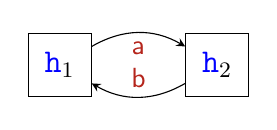
\begin{tikzpicture}[node distance=1.5cm,scale=1]
        \node (square-h) [draw,minimum width=0.8cm,minimum height=0.8cm] {\large $\hh_1$};
        \node (square-k) [draw,minimum width=0.8cm,minimum height=0.8cm, right of = square-h, xshift=5mm] {\large $\hh_2$};
       % 
      \path
      (square-h) edge[-stealth,bend left] node[below] {$\msg[a]$} (square-k)
      (square-k) edge[-stealth,bend left] node[above] {$\msg[b]$} (square-h)
      ;
 \end{tikzpicture}
 }
 %
 \hspace{8mm}
 %
\begin{array}{l}
\text{$\cs_2$}\\[12mm]
\end{array}
 \dbox{
 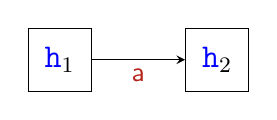
\begin{tikzpicture}[node distance=1.5cm,scale=1]
        \node (square-h) [draw,minimum width=0.8cm,minimum height=0.8cm] {\large $\hh_1$};
        \node (square-k) [draw,minimum width=0.8cm,minimum height=0.8cm, right of = square-h, xshift=5mm] {\large $\hh_2$};
       % 
      \path
      (square-h) edge[-stealth] node[below] {$\msg[a]$} (square-k)
      ;
 \end{tikzpicture} 
        }
 %
 \hspace{8mm}
 %
\begin{array}{l}
\text{$\cs_3$}\\[12mm]
\end{array}
 \dbox{
 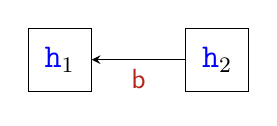
\begin{tikzpicture}[node distance=1.5cm,scale=1]
        \node (square-h) [draw,minimum width=0.8cm,minimum height=0.8cm] {\large $\hh_1$};
        \node (square-k) [draw,minimum width=0.8cm,minimum height=0.8cm, right of = square-h, xshift=5mm] {\large $\hh_2$};
       % 
      \path
      (square-k) edge[-stealth] node[below] {$\msg[b]$} (square-h)
      ;
 \end{tikzpicture} 
        }
 \end{equation}
%  $
% \caption{\label{fig:pcm} Three connection models for composing the systems in \cref{fig:twoipnterfaces}}
% }
%\end{figure}

Notice that the connection models depends only on the choosen interface interactions.
This holds however only for the binary case.
Not for the multicomposition (see below).

The following partial gateways can be obtained out of the interface participants and the connection
models.
\begin{equation}
\hspace{-8mm}
\begin{tikzpicture}[node distance=1.5cm,scale=1]
        \node (square-v)  [draw,minimum width=0.8cm,minimum height=0.8cm] {\large $\hh_3$};
        \node [state] (v-b) [left of = square-v, draw=none] {};
        \node [state] (v-a) [below of = square-v, draw=none] {};
        \draw [-stealth] (v-a) --  node {$\msg[a]$} (square-v);
        \draw [-stealth] (square-v) --  node {$\msg[b]$} (v-b);
        \node (square-w)  [draw,minimum width=0.8cm,minimum height=0.8cm, right of = square-v] {\large $\hh_4$};
        \node [state] (w-c) [right of = square-w, draw=none] {};
        \node [state] (w-a) [below of = square-w, draw=none] {};
        \node [state] (w-b) [above right of = square-w, draw=none] {};
        \draw [-stealth] (w-c) --  node {$\msg[c]$} (square-w);
        \draw [-stealth] (square-w) --  node {$\msg[a]$} (w-a);
        \draw [stealth-] (square-w) --  node {$\msg[b]$} (w-b);
        %
        \draw [-stealth] (square-w) to[out=-135,in=-45]  node {$\msg[b]$} (square-v);
        %
        \draw (0.4,0)[dotted,thick]  --  (0,-0.4); % carrying a inside v
        \draw (0.4,-0.4)[dotted,thick]  --  (-0.4,0); % carrying b inside v
        %
        \draw (1.5,0.4)[dotted,thick]  --  (1.5,-0.4); % carrying a inside w
        \draw (1.1,-0.4)[dotted,thick]  to[out=30,in=260]  (1.9,0.4); % carrying b inside w
        %
        %
        \draw [-stealth]  (0.4,0) to[out=45,in=90]  node [pos=0.6] {$\msg[a]$} (1.5,0.4 ); % carryng a from v to w  
 \end{tikzpicture}
 \hspace{0mm}
 \begin{tikzpicture}[node distance=1.5cm,scale=1]
        \node (square-v)  [draw,minimum width=0.8cm,minimum height=0.8cm] {\large $\hh_3$};
        \node [state] (v-b) [left of = square-v, draw=none] {};
        \node [state] (v-a) [below of = square-v, draw=none] {};
        \draw [-stealth] (v-a) --  node {$\msg[a]$} (square-v);
        \draw [-stealth] (square-v) --  node {$\msg[b]$} (v-b);
        \node (square-w)  [draw,minimum width=0.8cm,minimum height=0.8cm, right of = square-v] {\large $\hh_4$};
        \node [state] (w-c) [right of = square-w, draw=none] {};
        \node [state] (w-a) [below of = square-w, draw=none] {};
        \node [state] (w-b) [above right of = square-w, draw=none] {};
        \draw [-stealth] (w-c) --  node {$\msg[c]$} (square-w);
        \draw [-stealth] (square-w) --  node {$\msg[a]$} (w-a);
        \draw [stealth-] (square-w) --  node {$\msg[b]$} (w-b);
        %
        \draw [-stealth] (square-w) to[out=-135,in=-45]  node {$\msg[b]$} (square-v);
        %
        %\draw (0.4,0)[dotted,thick]  --  (0,-0.4); % carrying a inside v
        \draw (0.4,-0.4)[dotted,thick]  --  (-0.4,0); % carrying b inside v
        %
        %\draw (1.5,0.4)[dotted,thick]  --  (1.5,-0.4); % carrying a inside w
        \draw (1.1,-0.4)[dotted,thick]  to[out=30,in=260]  (1.9,0.4); % carrying b inside w
        %
        %
       % \draw [-stealth]  (0.4,0) to[out=45,in=90]  node [pos=0.6] {$\msg[a]$} (1.5,0.4 ); % carryng a from v to w  
 \end{tikzpicture}
 \hspace{0mm}
\begin{tikzpicture}[node distance=1.5cm,scale=1]
        \node (square-v)  [draw,minimum width=0.8cm,minimum height=0.8cm] {\large $\hh_3$};
        \node [state] (v-b) [left of = square-v, draw=none] {};
        \node [state] (v-a) [below of = square-v, draw=none] {};
        \draw [-stealth] (v-a) --  node {$\msg[a]$} (square-v);
        \draw [-stealth] (square-v) --  node {$\msg[b]$} (v-b);
        \node (square-w)  [draw,minimum width=0.8cm,minimum height=0.8cm, right of = square-v] {\large $\hh_4$};
        \node [state] (w-c) [right of = square-w, draw=none] {};
        \node [state] (w-a) [below of = square-w, draw=none] {};
        \node [state] (w-b) [above right of = square-w, draw=none] {};
        \draw [-stealth] (w-c) --  node {$\msg[c]$} (square-w);
        \draw [-stealth] (square-w) --  node {$\msg[a]$} (w-a);
        \draw [stealth-] (square-w) --  node {$\msg[b]$} (w-b);
        %
        %\draw [-stealth] (square-w) to[out=-135,in=-45]  node {$\msg[b]$} (square-v);
        %
        \draw (0.4,0)[dotted,thick]  --  (0,-0.4); % carrying a inside v
        %\draw (0.4,-0.4)[dotted,thick]  --  (-0.4,0); % carrying b inside v
        %
        \draw (1.5,0.4)[dotted,thick]  --  (1.5,-0.4); % carrying a inside w
        %
        %
        \draw [-stealth]  (0.4,0) to[out=45,in=90]  node [pos=0.6] {$\msg[a]$} (1.5,0.4 ); % carryng a from v to w  
 \end{tikzpicture}
\end{equation}

In general, not any choice of interface actions makes sense. 
Let consider an interface like $\hh_2$ below.

\begin{equation}
 \begin{tikzpicture}[node distance=1.5cm,scale=1]
        \node (square-k) [draw,minimum width=0.8cm,minimum height=0.8cm] {\large $\hh_2$};
        \node [state] (k-b) [above right of = square-k, draw=none] {};
        \node [state] (k-a) [below right of = square-k, draw=none, xshift=2mm] {};
        %\draw [stealth-] (k-b) --  node[right] {$\msg[inf]$} (square-k);
        \draw [-stealth] (0.4,0) --  node[right] {$\msg[a]$} (k-a);
        \draw  [-stealth] (0.4,0)   --  node [right] {$\msg[b]$} (k-b);
 \end{tikzpicture}
\end{equation} 
Let us also assume that there exists an actual branch for $\msg[a]$ and  $\msg[b]$ 
in the the dynamic specification of $\hh_2$ (a CFSM communicating asynchronous by meas of channes).
In such a case, the following choice of interface actions would not make sense.

\begin{equation}
 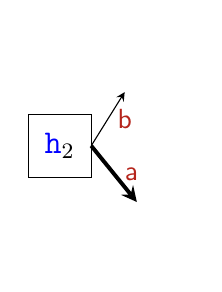
\begin{tikzpicture}[node distance=1.5cm,scale=1]
        \node (square-k) [draw,minimum width=0.8cm,minimum height=0.8cm] {\large $\hh_2$};
        \node [state] (k-b) [above right of = square-k, draw=none] {};
        \node [state] (k-a) [below right of = square-k, draw=none, xshift=2mm] {};
        %\draw [stealth-] (k-b) --  node[right] {$\msg[inf]$} (square-k);
        \draw [-stealth,line width=0.5mm] (0.4,0) --  node[right] {$\msg[a]$} (k-a);
        \draw  [-stealth] (0.4,0)   --  node [right] {$\msg[b]$} (k-b);
 \end{tikzpicture}
\end{equation}
The above in fact implies that, when in a composition we substitute the interface $\hh_2$ with a 
partial gateway, the latter should make a decision between acting as a forwarder
or as the producer of a piece of information.
In the latter case, the partial gateway would have no means to prevent other 
gateways to insert a message $\msg[a]$ in a communication channel.
So, it could occur that a message $\msg[a]$ stays forever in the channel,
so disrupting some communication properties of the system obtained by composition.
We shall require a syntactic condition to be satisfied in order issues like the one
intuitively described above cannot occur.

\bigskip

The PaI approach to binary composition via partial gateways that we have described above 
scales up to general multiple composition easily. 
Let us consider an example from~\cite{BDGY23} having four systems $S_1$,  $S_2$, $S_3$ and $S_4$.
As shown in (\ref{eq:four-ips}) below, we have selected for each system one participant
as an interface, named respectively $\hh_1$, $\hh_2$, $\hh_3$ and $\hh_4$.
 
%\begin{wrapfigure}{r}{0.45\textwidth}
%\begin{figure}[h]
%    %\vspace{-8mm}
%     \centering{\small
%    $
\begin{equation}
\label{eq:four-ips}
    \begin{array}{@{\hspace{0mm}}c@{\hspace{-2mm}}}
    \begin{array}{c@{\hspace{-2mm}}c}
    \text{\large $S_1$}
    &
 \begin{tikzpicture}[node distance=1.5cm,scale=1]
        \node (square-h) [draw,minimum width=0.8cm,minimum height=0.8cm] {\large $\hh_1$};
        \node [state] (h-a) [above of = square-h, draw=none] {};
        \node [state] (h-c) [left of = square-h, draw=none] {};
        \draw [-stealth] (h-a) --  node {$\msg[a]$} (square-h);
        \draw [-stealth] (square-h) --  node {$\msg[c]$} (h-c);
 \end{tikzpicture}
 \end{array}
 \hspace{4mm}
\begin{array}{c}
 \\
 \\
| \\
| \\
|\\
|\\
\end{array}
 \hspace{4mm}
 \begin{array}{c@{\hspace{-2mm}}c}
\begin{tikzpicture}[node distance=1.5cm,scale=1]
        \node (square-k) [draw,minimum width=0.8cm,minimum height=0.8cm] {\large $\hh_2$};
        \node [state] (k-b) [above of = square-k, draw=none] {};
        \node [state] (k-a) [right of = square-k, draw=none] {};
        \draw [-stealth] (k-b) --  node {$\msg[b]$} (square-k);
        \draw [-stealth] (square-k) --  node {$\msg[a]$} (k-a);
 \end{tikzpicture}
 &
 \text{\large $S_2$} 
 \end{array}
 \\[12mm]
\hspace{3mm}- - - -    \hspace{8mm}- - - - -  \\[-5mm]
\begin{array}{@{\hspace{0mm}}c@{\hspace{0mm}}c}
\\[4mm]
\text{\large $S_3\hspace{-2mm}$} 
&
 \begin{tikzpicture}[node distance=1.5cm,scale=1]
        \node (square-v) [draw,minimum width=0.8cm,minimum height=0.8cm] {\large $\hh_3$};
        \node [state] (v-b) [left of = square-v, draw=none] {};
        \node [state] (v-a) [below of = square-v, draw=none] {};
        \draw [-stealth] (v-a) --  node {$\msg[a]$} (square-v);
        \draw [-stealth] (square-v) --  node {$\msg[b]$} (v-b);
 \end{tikzpicture}
 \end{array}
 \hspace{4mm}
\begin{array}{c}
 \\[-8mm]
| \\
| \\
| \\
|
\end{array}
 \hspace{4mm}
 \begin{array}{c@{\hspace{-2mm}}}
 \\[-6mm]
 \begin{tikzpicture}[node distance=1.5cm,scale=1]
        \node (square-w) [draw,minimum width=0.8cm,minimum height=0.8cm] {\large $\hh_4$};
        \node [state] (w-c) [right of = square-w, draw=none] {};
        \node [state] (w-a) [below of = square-w, draw=none] {};
        \node [state] (w-b) [above right of = square-w, draw=none] {};
        \draw [-stealth] (w-c) --  node {$\msg[c]$} (square-w);
        \draw [-stealth] (square-w) --  node {$\msg[a]$} (w-a);
        \draw [stealth-] (square-w) --  node {$\msg[b]$} (w-b);
 \end{tikzpicture}
 \hspace{-6mm}
 \begin{array}{l}
 \\[6mm]
 \text{\large\ \ $S_4$}
 \end{array} 
 \end{array}
 \\[-4mm]
 \end{array}
 \end{equation}
% $
% }
%\caption{\label{fig:four-ips}
%Four systems with their respective interface participants}
% \end{figure}
% \vspace{-5mm}
% \end{wrapfigure}

We could take into account the following interface actions.

%\begin{figure}[h]
%    %\vspace{-8mm}
%     \centering{\small
%    $
\begin{equation}
\label{eq:four-ips}
    \begin{array}{@{\hspace{0mm}}c@{\hspace{-2mm}}}
    \begin{array}{c@{\hspace{-2mm}}c}
    \text{\large $S_1$}
    &
 \begin{tikzpicture}[node distance=1.5cm,scale=1]
        \node (square-h) [draw,minimum width=0.8cm,minimum height=0.8cm] {\large $\hh_1$};
        \node [state] (h-a) [above of = square-h, draw=none] {};
        \node [state] (h-c) [left of = square-h, draw=none] {};
        \draw [-stealth,line width=0.5mm] (h-a) --  node [right] {$\msg[a]$} (square-h);
        \draw [-stealth] (square-h) --  node {$\msg[c]$} (h-c);
 \end{tikzpicture}
 \end{array}
 \hspace{4mm}
\begin{array}{c}
 \\
 \\
| \\
| \\
|\\
|\\
\end{array}
 \hspace{4mm}
 \begin{array}{c@{\hspace{-2mm}}c}
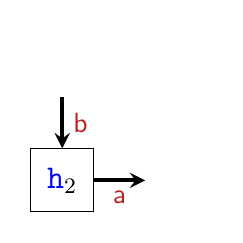
\begin{tikzpicture}[node distance=1.5cm,scale=1]
        \node (square-k) [draw,minimum width=0.8cm,minimum height=0.8cm] {\large $\hh_2$};
        \node [state] (k-b) [above of = square-k, draw=none] {};
        \node [state] (k-a) [right of = square-k, draw=none] {};
        \draw [-stealth, line width=0.5mm] (k-b) --  node [right] {$\msg[b]$} (square-k);
        \draw [-stealth, line width=0.5mm] (square-k) --  node [below] {$\msg[a]$} (k-a);
 \end{tikzpicture}
 &
 \text{\large $S_2$} 
 \end{array}
 \\[12mm]
\hspace{3mm}- - - -    \hspace{8mm}- - - - -  \\[-5mm]
\begin{array}{@{\hspace{0mm}}c@{\hspace{0mm}}c}
\\[4mm]
\text{\large $S_3\hspace{-2mm}$} 
&
 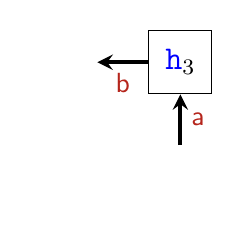
\begin{tikzpicture}[node distance=1.5cm,scale=1]
        \node (square-v) [draw,minimum width=0.8cm,minimum height=0.8cm] {\large $\hh_3$};
        \node [state] (v-b) [left of = square-v, draw=none] {};
        \node [state] (v-a) [below of = square-v, draw=none] {};
        \draw [-stealth,line width=0.5mm] (v-a) --  node [right]   {$\msg[a]$} (square-v);
        \draw [-stealth,line width=0.5mm] (square-v) --  node [below] {$\msg[b]$} (v-b);
 \end{tikzpicture}
 \end{array}
 \hspace{4mm}
\begin{array}{c}
 \\[-8mm]
| \\
| \\
| \\
|
\end{array}
 \hspace{4mm}
 \begin{array}{c@{\hspace{-2mm}}}
 \\[-6mm]
 \begin{tikzpicture}[node distance=1.5cm,scale=1]
        \node (square-w) [draw,minimum width=0.8cm,minimum height=0.8cm] {\large $\hh_4$};
        \node [state] (w-c) [right of = square-w, draw=none] {};
        \node [state] (w-a) [below of = square-w, draw=none] {};
        \node [state] (w-b) [above right of = square-w, draw=none] {};
        \draw [-stealth] (w-c) --  node {$\msg[c]$} (square-w);
        \draw [-stealth,line width=0.5mm] (square-w) --  node [right] {$\msg[a]$} (w-a);
        \draw [stealth-] (square-w) --  node {$\msg[b]$} (w-b);
 \end{tikzpicture}
 \hspace{-6mm}
 \begin{array}{l}
 \\[6mm]
 \text{\large\ \ $S_4$}
 \end{array} 
 \end{array}
 \\[-4mm]
 \end{array}
 \end{equation}
% $
% }
%\caption{\label{fig:four-ips}
%Four interfaces with particular interface actions.}
% \end{figure}
% \vspace{-5mm}
% \end{wrapfigure}

Unlike the binary case, a connection policy is not uniquely determined the specification
of which are the interface actions in the interface participants.

For what concerns  the choice of interface actions highlighted in (\ref{eq:four-ips}),
 one could decide that message $\msg[a]$ received by $\hh_1$ has 
 to be forwarded
 to $\hh_4$; the $\msg[a]$ received by $\hh_3$
 to $\hh_2$; the $\msg[b]$ received by $\hh_2$ to $\hh_3$.
 Another possible choice 
could be similar to the previous one but for the forwarding
of the messages $\msg[a]$: the one received by $\HH_1$ could be forwarded now to $\hh_2$
whereas the one received by $\hh_3$ could be forwarded to $\hh_4$. 
So, it is possible to have the following two connection models, both coherent
with the interface actions highlighted in (\ref{fig:four-ips}).  
 

%%% CONNECTION MODELS
% \begin{figure}[ht]
%    \centering{
 \begin{equation}
    \raisebox{15mm}{$\cs_\mathrm{A}$}
    \begin{array}{c@{\qquad\qquad\qquad\qquad\qquad}c}
\dbox{
 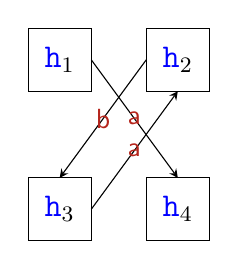
\begin{tikzpicture}[node distance=1.5cm,scale=1]
        \node (square-h) [draw,minimum width=0.8cm,minimum height=0.8cm] {\large $\hh_1$};
        \node (square-k) [draw,minimum width=0.8cm,minimum height=0.8cm, right of = square-h] {\large $\hh_2$};
        \node (square-v)  [draw,minimum width=0.8cm,minimum height=0.8cm, below of = square-h, yshift=-4mm] {\large $\hh_3$};
        \node (square-w)  [draw,minimum width=0.8cm,minimum height=0.8cm, below of = square-k, yshift=-4mm] {\large $\hh_4$};
        %\draw[-stealth]  (square-w) to[out=-135,in=-45]  node {$\msg[b]$} (square-v);
        %
        %
        \draw [-stealth] (0.4,0)  -- node {$\msg[a]$}  (1.5,-1.5 ); % carryng a from h to w    
        % \draw [stealth-] (0,-0.4)  -- node {$\msg[c]$} (1.1,-1.9); % carryng c from w to h 
        \draw [-stealth] (0.4,-1.9)  --  node {$\msg[a]$} (1.5,-0.4 ); % carrying a from v to k
        \draw [stealth-] (0,-1.5)  --  node {$\msg[b]$} (1.1,0); % carrying  b from k to v
 \end{tikzpicture}
 }
&
\dbox{
 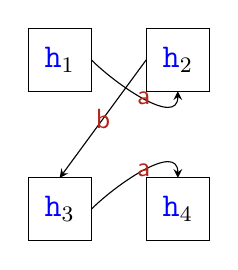
\begin{tikzpicture}[node distance=1.5cm,scale=1]
        \node (square-h) [draw,minimum width=0.8cm,minimum height=0.8cm] {\large $\HH_1$};
        \node (square-k) [draw,minimum width=0.8cm,minimum height=0.8cm, right of = square-h] {{\large $\hh_2$}};
        \node (square-v)  [draw,minimum width=0.8cm,minimum height=0.8cm, below of = square-h, yshift=-4mm] {{\large $\hh_3$}};
        \node (square-w)  [draw,minimum width=0.8cm,minimum height=0.8cm, below of = square-k, yshift=-4mm] {{\large $\hh_4$}};
        %
        %\draw [-stealth] (square-w) to[out=-135,in=-45]  node {$\msg[b]$} (square-v);
        %
        %
        \draw [-stealth] (0.4,-1.9) to[out=45,in=90] node {$\msg[a]$} (1.5,-1.5 ); % carryng a from v to w    
         %\draw [stealth-] (0,-0.4)  -- node {$\msg[c]$} (1.1,-1.9) ; % carryng c from w to h 
        \draw [-stealth]  (0.4,0)  to[out=-45,in=-90]  node {$\msg[a]$} (1.5,-0.4 ); % carrying a from h to k
        %\draw [-stealth]  (square-v)  to[out=45,in=-90]  node {$\msg[a]$} (square-k); % carrying a from h to k
        \draw [stealth-] (0,-1.5)  --  node {$\msg[b]$} (1.1,0); % carrying  b from k to v
 \end{tikzpicture}
 }
 \raisebox{14.5mm}{$\,\,\,\,\cs_\mathrm{B}$}
 \end{array}
  \end{equation}
% $
% }
% \caption{\label{fig:choicesAB} Two connection models for multicomposition.}\label{fig:twocm}
% \end{figure}
 
 \noindent
  Similarly to the binary case, the PaI multicomposition via partial gateways of the four
 systems consists in fact in replacing the participants  $\hh_1$, $\hh_2$, $\hh_3$ and $\hh_4$, chosen  as
interfaces, by gateways whose task stays the same for what concerns the non interface-actions,
whereas messages of interfaces actions are simply forwarded.
 The  architecture  of the resulting composed systems, according to the connection models is
represented  by the diagrams  in (\ref{eq:multiconnection}),  where the names $\hh_1, \hh_2, \hh_3$
and $\hh_4$ are now partial gateways.
%\begin{figure}[h]%{c}{0.6\textwidth}
%\vspace{-4mm}
%    \centering{
\vspace{-4mm} 
\begin{equation}
 \label{eq:multiconnection}
    \begin{array}{c@{\quad\qquad}c}
 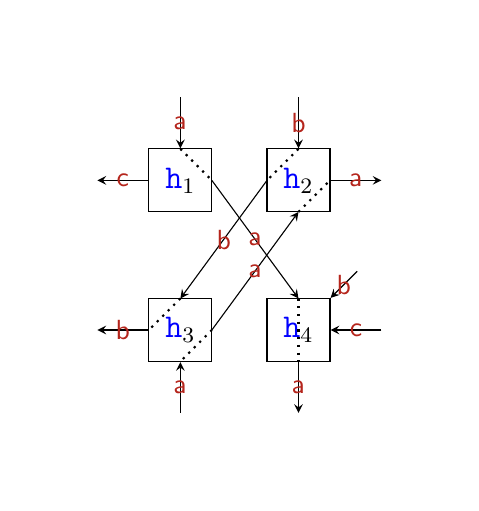
\begin{tikzpicture}[node distance=1.5cm,scale=1]
        \node (square-h) [draw,minimum width=0.8cm,minimum height=0.8cm] {\large $\hh_1$};
        \node [state] (h-a) [above of = square-h, draw=none] {};
        \node [state] (h-c) [left of = square-h, draw=none] {};
        \draw [-stealth] (h-a) --  node {$\msg[a]$} (square-h);
        \draw [-stealth] (square-h) --  node {$\msg[c]$} (h-c);
        \node (square-k) [draw,minimum width=0.8cm,minimum height=0.8cm, right of = square-h] {\large $\hh_2$};
        \node [state] (k-b) [above of = square-k, draw=none] {};
        \node [state] (k-a) [right of = square-k, draw=none] {};
        \draw [-stealth] (k-b) --  node {$\msg[b]$} (square-k);
        \draw [-stealth] (square-k) --  node {$\msg[a]$} (k-a);
        \node (square-v)  [draw,minimum width=0.8cm,minimum height=0.8cm, below of = square-h, yshift=-4mm] {\large $\hh_3$};
        \node [state] (v-b) [left of = square-v, draw=none] {};
        \node [state] (v-a) [below of = square-v, draw=none] {};
        \draw [-stealth] (v-a) --  node {$\msg[a]$} (square-v);
        \draw [-stealth] (square-v) --  node {$\msg[b]$} (v-b);
        \node (square-w)  [draw,minimum width=0.8cm,minimum height=0.8cm, below of = square-k, yshift=-4mm] {\large $\hh_4$};
        \node [state] (w-c) [right of = square-w, draw=none] {};
        \node [state] (w-a) [below of = square-w, draw=none] {};
        \node [state] (w-b) [above right of = square-w, draw=none] {};
        \draw [-stealth] (w-c) --  node {$\msg[c]$} (square-w);
        \draw [-stealth] (square-w) --  node {$\msg[a]$} (w-a);
        \draw [stealth-] (square-w) --  node {$\msg[b]$} (w-b);
        %
      %  \draw (square-h)  to[out=-90,in=90]   node {} (square-w);
       % \draw (square-k) to[out=-90,in=90]  node {} (square-v);
      %  \draw (square-h) to[out=0,in=180]  node {} (square-w);
      %  \draw [-stealth] (square-w) to[out=-135,in=-45]  node {$\msg[b]$} (square-v);
      %  \draw (square-k) to[out=-135,in=45]  node {} (square-v);
        %
        \draw (0,0.4)[dotted,thick]  --  (0.4,0); % carrying a inside h  
        %\draw (-0.4,0)[dotted,thick]  --  (0,-0.4); % carrying c inside h
        %
        \draw (1.5,0.4)[dotted,thick]  --  (1.1,0); % carrying b inside k
        \draw (1.5,-0.4)[dotted,thick]  --  (1.9,0); % carrying a inside k
        %
        \draw (0.4,-1.9)[dotted,thick]  --  (0,-2.3); % carrying a inside v
        \draw (0,-1.5)[dotted,thick]  --  (-0.4,-1.9); % carrying k's b inside v
        %\draw (0.4,-2.3)[dotted,thick]  --  (-0.4,-1.9); % carrying b inside v
        %
        \draw (1.5,-1.5)[dotted,thick]  --  (1.5,-2.3); % carrying a inside w
        %\draw (1.1,-1.9)[dotted,thick]  --  (1.9,-1.9); % carrying c inside w
        %\draw (1.1,-2.3)[dotted,thick]  to[out=30,in=260]  (1.9,-1.5); % carrying b inside w
        %
        %
        \draw[-stealth]   (0.4,0)  -- node  {$\msg[a]$}   (1.5,-1.5 ); % carryng a from h to w    
         %\draw  [stealth-]  (0,-0.4)  --  node  {$\msg[c]$}  (1.1,-1.9); % carryng c from w to h 
        \draw [-stealth]  (0.4,-1.9)  --   node  {$\msg[a]$} (1.5,-0.4 ); % carrying a from v to k
        \draw [stealth-]  (0,-1.5)  --  node {$\msg[b]$} (1.1,0); % carrying  b from k to v
 \end{tikzpicture}
& 
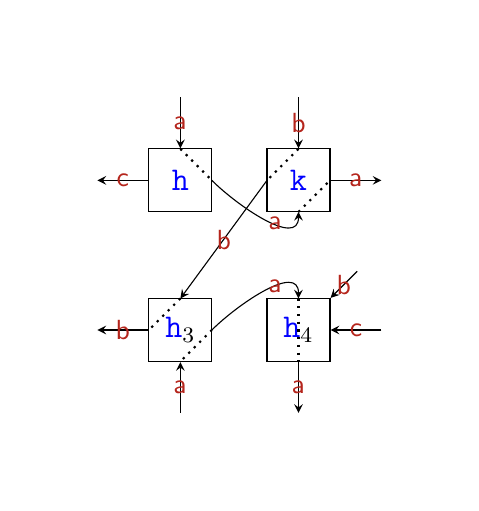
\begin{tikzpicture}[node distance=1.5cm,scale=1]
        \node (square-h) [draw,minimum width=0.8cm,minimum height=0.8cm] {\large $\HH$};
        \node [state] (h-a) [above of = square-h, draw=none] {};
        \node [state] (h-c) [left of = square-h, draw=none] {};
        \draw [-stealth] (h-a) --  node {$\msg[a]$} (square-h);
        \draw [-stealth] (square-h) --  node {$\msg[c]$} (h-c);
        \node (square-k) [draw,minimum width=0.8cm,minimum height=0.8cm, right of = square-h] {\large $\KK$};
        \node [state] (k-b) [above of = square-k, draw=none] {};
        \node [state] (k-a) [right of = square-k, draw=none] {};
        \draw [-stealth] (k-b) --  node {$\msg[b]$} (square-k);
        \draw [-stealth] (square-k) --  node {$\msg[a]$} (k-a);
        \node (square-v)  [draw,minimum width=0.8cm,minimum height=0.8cm, below of = square-h, yshift=-4mm] {\large $\hh_3$};
        \node [state] (v-b) [left of = square-v, draw=none] {};
        \node [state] (v-a) [below of = square-v, draw=none] {};
        \draw [-stealth] (v-a) --  node {$\msg[a]$} (square-v);
        \draw [-stealth] (square-v) --  node {$\msg[b]$} (v-b);
        \node (square-w)  [draw,minimum width=0.8cm,minimum height=0.8cm, below of = square-k, yshift=-4mm] {\large $\hh_4$};
        \node [state] (w-c) [right of = square-w, draw=none] {};
        \node [state] (w-a) [below of = square-w, draw=none] {};
        \node [state] (w-b) [above right of = square-w, draw=none] {};
        \draw [-stealth] (w-c) --  node {$\msg[c]$} (square-w);
        \draw [-stealth] (square-w) --  node {$\msg[a]$} (w-a);
        \draw [stealth-] (square-w) --  node {$\msg[b]$} (w-b);
        %
        %\draw [-stealth] (square-w) to[out=-135,in=-45]  node {$\msg[b]$} (square-v);
        %
        \draw (0,0.4)[dotted,thick]  --  (0.4,0); % carrying a inside h  
        %\draw (-0.4,0)[dotted,thick]  --  (0,-0.4); % carrying c inside h
        %
        \draw (1.5,0.4)[dotted,thick]  --  (1.1,0); % carrying b inside k
        \draw (1.5,-0.4)[dotted,thick]  --  (1.9,0); % carrying a inside k
        %
        \draw (0.4,-1.9)[dotted,thick]  --  (0,-2.3); % carrying a inside v
        \draw (0,-1.5)[dotted,thick]  --  (-0.4,-1.9); % carrying k's b inside v
        %\draw (0.4,-2.3)[dotted,thick]  --  (-0.4,-1.9); % carrying b inside v
        %
        \draw (1.5,-1.5)[dotted,thick]  --  (1.5,-2.3); % carrying a inside w
        %\draw (1.1,-1.9)[dotted,thick]  --  (1.9,-1.9); % carrying c inside w
        %\draw (1.1,-2.3)[dotted,thick]  to[out=30,in=260]  (1.9,-1.5); % carrying b inside w
        %
        %
        \draw [-stealth]  (0.4,-1.9) to[out=45,in=90]  node [pos=0.6] {$\msg[a]$} (1.5,-1.5 ); % carryng a from v to w    
         %\draw [stealth-]  (0,-0.4)  --  node  {$\msg[c]$} (1.1,-1.9); % carryng c from w to h 
        \draw [-stealth]  (0.4,0)  to[out=-45,in=-90]  node [pos=0.6]  {$\msg[a]$} (1.5,-0.4 ); % carrying a from h to k
        \draw [stealth-]  (0,-1.5)  -- node  {$\msg[b]$}  (1.1,0); % carrying  b from k to v
 \end{tikzpicture}\\[-4mm]
 \text{\small (Using $\cs_\mathrm{A}$)}
 &
 \text{\small (Using $\cs_\mathrm{B}$)}
 \end{array}
  \end{equation}
 
%  }
%  \vspace{-1mm}
%  \caption{Static description of two PaI multicompositions via partial gateways}
%  \label{fig:multiconnection}
% \end{figure}

One of the main results of the paper is that a number of comminication properties
are preserved by PaI multicomposition via partial gateways in case the very same
properties are enjoied by the connection policy used for the composition.
Such a result is actually obtained as a corollary of a preservation result for 
a restricted form of binary PaI composition that we dub partial-fusion PaI composition.
All forms of PaI composition for asynchronous CFSM can be obtained by a number
of binary partial-fusion PaI composition, which can hence be considered as the 
basis of the PaI approach.

\paragraph{Partial Fusion PaI Composition}

This particular form of PaI composition is binary.
To get an intuitive idea of that, let us consider the following simple example, where
both $S_1$ and $S_2$ possess a participant named $\hh$ that we choose as
their respective interface participant.

\begin{equation}
\label{eq:exps}
\raisebox{2mm}{\text{\large $S_1$}\,\,}
%    \dbox{
\hspace{10mm} \begin{tikzpicture}[node distance=1.5cm,scale=1]
        \node (square-h) [draw,minimum width=0.8cm,minimum height=0.8cm] {\large $\hh$};
        \node [state] (h-a) [above of = square-h, draw=none] {};
        \node [state] (h-c) [left of = square-h, draw=none, xshift=-2mm] {};
        \draw [-stealth] (h-a) --  node {$\msg[a]$} (square-h);
        \draw [stealth-] (h-c) --  node {$\msg[b]$} (square-h);
 \end{tikzpicture}
%            }
\hspace{2mm}
 \begin{array}{c}
 \\[8mm]
| \\
| \\
|\\
|\\
\end{array}
\hspace{4mm}
%     \dbox{
 \begin{tikzpicture}[node distance=1.5cm,scale=1]
        \node (square-k) [draw,minimum width=0.8cm,minimum height=0.8cm] {\large $\hh$};
        \node [state] (k-b) [above of = square-k, draw=none] {};
        \node [state] (k-a) [right of = square-k, draw=none] {};
        %\draw [stealth-] (k-b) --  node[right] {$\msg[inf]$} (square-k);
        \draw [-stealth] (square-k) --  node {$\msg[a]$} (k-a);
       % \draw  [-stealth] (0.4,-0.2)   --  node [below] {$\msg[par]$} (1.2,-0.2);
 \end{tikzpicture} \hspace{18mm}
 %            }
 \raisebox{0mm}{\text{\large $\,\,S_2$}}
 \end{equation}
 
The composition method requires that some interaction actions are choosen in only one
of the two interface participants.  

\begin{equation}
\label{eq:expsia}
\begin{array}{c}
\\[-18mm]
\raisebox{2mm}{\text{\large $S_1$}\,\,}
%    \dbox{
\hspace{10mm} \begin{tikzpicture}[node distance=1.5cm,scale=1]
        \node (square-h) [draw,minimum width=0.8cm,minimum height=0.8cm] {\large $\hh$};
        \node [state] (h-a) [above of = square-h, draw=none] {};
        \node [state] (h-c) [left of = square-h, draw=none, xshift=-2mm] {};
        \draw [-stealth,line width=0.5mm] (h-a) --  node[right] {$\msg[a]$} (square-h);
        \draw [stealth-] (h-c) --  node {$\msg[b]$} (square-h);
 \end{tikzpicture}
%            }
\hspace{2mm}
 \begin{array}{c}
 \\[8mm]
| \\
| \\
|\\
|\\
\end{array}
\hspace{4mm}
%     \dbox{
 \begin{tikzpicture}[node distance=1.5cm,scale=1]
        \node (square-k) [draw,minimum width=0.8cm,minimum height=0.8cm] {\large $\hh$};
        \node [state] (k-b) [above of = square-k, draw=none] {};
        \node [state] (k-a) [right of = square-k, draw=none] {};
        %\draw [stealth-] (k-b) --  node[right] {$\msg[inf]$} (square-k);
        \draw [-stealth] (square-k) --  node {$\msg[a]$} (k-a);
       % \draw  [-stealth] (0.4,-0.2)   --  node [below] {$\msg[par]$} (1.2,-0.2);
 \end{tikzpicture} \hspace{18mm}
 %            }
 \raisebox{0mm}{\text{\large $\,\,S_2$}}
 \end{array}
 \end{equation}

We ``restrict'' now the behaviour of  $\hh$ in $S_1$ (the interface participant with interface actions)
to its interface actions only.
\begin{equation}
\begin{array}{c}
\\[-18mm]
\begin{tikzpicture}[node distance=1.5cm,scale=1]
        \node (square-h) [draw,minimum width=0.8cm,minimum height=0.8cm] {\large $\hh'$};
        \node [state] (h-a) [above of = square-h, draw=none] {};
        \node [state] (h-c) [left of = square-h, draw=none, xshift=-2mm] {};
        \draw [-stealth] (h-a) --  node {$\msg[a]$} (square-h);
 \end{tikzpicture}
  \end{array}
\end{equation}

The composition can be carried on now, since $\hh'$ above and $\hh$ of $S_2$ in (\ref{eq:expsia}) 
are dual (one has an input where the other has an output end vice versa).
 Such a duality property enables to (partially) fuse together the $\hh$ in $S_1$ with the
 $\hh$ in $S_2$ so obtaining a composed system.
 The fusion makes $\hh$ a single and (partially) forwarding gateway: the messages pertaining to
 interface actions are forwarded, whereas such a partial gateways keeps on behaving as the $\hh$ of $S_1$ for what concerns the non interface-actions.

\begin{equation}
\label{fig:bincomp}
\begin{array}{l}
\text{\large $S_1$}\!\stackrel{\hh}{ \mathtt{fuse}}\text{\large $S_2$}\\[12mm]
\end{array}
\hspace{12mm}
% \dbox{ \hspace{28mm}
 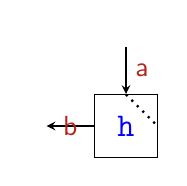
\begin{tikzpicture}[node distance=1.5cm,scale=1]
        \node (square-h) [draw,minimum width=0.8cm,minimum height=0.8cm] {\large $\hh$};
         \node[draw=none,fill=none] (h-a) [above = 6mm  of square-h]{};
         \node[draw=none,fill=none] (a-h) [left = 6mm  of square-h]{};
        \draw [-stealth] (h-a) --  node [right] {$\msg[a]$} (square-h);
        \draw [-stealth] (square-h) --  node {$\msg[b]$} (a-h);
         %
        \draw (0,0.4)[dotted,thick]  --  (0.4,0); 
 \end{tikzpicture}
 \hspace{22mm}
%       }
\end{equation}

\medskip

We prove that fusion-composition preserve a number of communication properties.
Besides, it is possible to show that PaI composition by partial gateways (and hence 
PaI composition by gateways in general) preserve such properties since any 
PaI composition (binary, with multiple systems, orchestrated) simply reduces
to a number of fusion compositions.
We show that with an example for the binary case for the sake of simplicity.
Let us consider the systems $S_1$ and $S_2$ as in (\ref{eq:twointerfaces})
We hence consider the following identification of interface actions.
\begin{equation}
\label{eq:simpleexia}
\begin{array}{c}
\\[-18mm]
\raisebox{4mm}{\text{\large $S_1$}\,\,}
%    \dbox{
\hspace{10mm} \begin{tikzpicture}[node distance=1.5cm,scale=1]
        \node (square-h) [draw,minimum width=0.8cm,minimum height=0.8cm] {\large $\hh_1$};
        \node [state] (h-a) [above of = square-h, draw=none] {};
        \node [state] (h-c) [left of = square-h, draw=none, xshift=-2mm] {};
        \draw [-stealth,line width=0.5mm] (h-a) --  node[right] {$\msg[sbs]$} (square-h);
        \draw [stealth-] (h-c) --  node[above] {$\msg[inf]$} (square-h);
 \end{tikzpicture}
%            }
\hspace{2mm}
 \begin{array}{c}
 \\[8mm]
| \\
| \\
|\\
|\\
\end{array}
\hspace{4mm}
%     \dbox{
 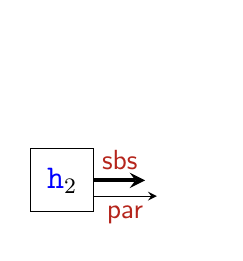
\begin{tikzpicture}[node distance=1.5cm,scale=1]
        \node (square-k) [draw,minimum width=0.8cm,minimum height=0.8cm] {\large $\hh_2$};
        \node [state] (k-b) [above of = square-k, draw=none] {};
        \node [state] (k-a) [right of = square-k, draw=none] {};
        %\draw [stealth-] (k-b) --  node[right] {$\msg[inf]$} (square-k);
        \draw [-stealth,line width=0.5mm] (square-k) --  node[above] {$\msg[sbs]$} (k-a);
        \draw  [-stealth] (0.4,-0.2)   --  node [below] {$\msg[par]$} (1.2,-0.2);
 \end{tikzpicture} \hspace{18mm}
 %            }
 \raisebox{2mm}{\text{\large $\,\,S_2$}}
 \end{array}
 \end{equation}
 

Since we are considering a binary case, the connection policy is uniquely determined.

%\begin{figure}[h]
%    \centering{\small
%    $
\begin{equation}
\label{fig:pcp}
\begin{array}{l}
\text{$\cs$}\\[12mm]
\end{array}
 \dbox{
 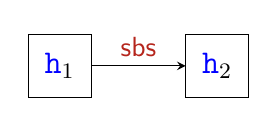
\begin{tikzpicture}[node distance=1.5cm,scale=1]
        \node (square-h) [draw,minimum width=0.8cm,minimum height=0.8cm] {\large $\hh_1$};
        \node (square-k) [draw,minimum width=0.8cm,minimum height=0.8cm, right of = square-h, xshift=5mm] {\large $\hh_2$};
         %
        \draw [-stealth] (0.4,0)  --  node [above] {$\msg[sbs]$} (1.6,0); % carrying sbs from h1 to h2 h2
 \end{tikzpicture}
 }
 \end{equation}
% $
% \caption{\label{fig:pcp} A connection policy for composing the systems in \cref{fig:twoipnterfaces}}
% }
%\end{figure}

Now we consider systems $S_1$ and $\cs$ (recall that also $\cs$ is a system).

% \begin{figure}[h]
%    \centering{\small
%    $
\begin{equation}
\label{fig:twoipnterfaces}
\raisebox{10mm}{\text{\large $S_1$}\,\,}
    \dbox{
\hspace{10mm} \begin{tikzpicture}[node distance=1.5cm,scale=1]
        \node (square-h) [draw,minimum width=0.8cm,minimum height=0.8cm] {\large $\hh_1$};
        \node [state] (h-a) [above of = square-h, draw=none] {};
        \node [state] (h-c) [left of = square-h, draw=none, xshift=-2mm] {};
        \draw [-stealth] (h-a) --  node[right] {$\msg[sbs]$} (square-h);
        \draw [stealth-] (h-c) --  node[above] {$\msg[inf]$} (square-h);
 \end{tikzpicture}
            }
\hspace{12mm}
 \begin{array}{l}
\text{$\cs$}\\[12mm]
\end{array}
 \dbox{
 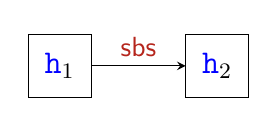
\begin{tikzpicture}[node distance=1.5cm,scale=1]
        \node (square-h) [draw,minimum width=0.8cm,minimum height=0.8cm] {\large $\hh_1$};
        \node (square-k) [draw,minimum width=0.8cm,minimum height=0.8cm, right of = square-h, xshift=5mm] {\large $\hh_2$};
         %
        \draw [-stealth] (0.4,0)  --  node [above] {$\msg[sbs]$} (1.6,0); % carrying sbs from h1 to h2 h2
 \end{tikzpicture}
 }
 \end{equation}
% $\vspace{-2mm}
% \caption{\label{fig:twoipnterfaces} Two interfaces participants belonging to, respectively, systems $S_1$ and $S_2$.}
% }
%\end{figure}

The above system are elegible for fusion composition, which returns the following system.

%\begin{figure}[h]
%    \centering{\small
%    $
\begin{equation}
\label{fig:binpcomp}
\begin{array}{l}
\text{\large $S_1$}\!\stackrel{\hh_1}{ \mathtt{fuse}}\cs\\[22mm]
\end{array}
 \dbox{ \hspace{28mm}
 \begin{tikzpicture}[node distance=1.5cm,scale=1]
        \node (square-h) [draw,minimum width=0.8cm,minimum height=0.8cm] {\large $\hh_1$};
        \draw [-stealth] (h-a) --  node [right] {$\msg[sbs]$} (square-h);
        \node (square-k) [draw,minimum width=0.8cm,minimum height=0.8cm, right of = square-h, xshift=5mm] {\large $\hh_2$};
         \node[draw=none,fill=none] (phantom) [above = 12mm  of square-h]{};
         \node[draw=none,fill=none] (phantom2) [left = 10mm  of square-h]{};
        \draw [stealth-] (phantom2) --  node [above]{$\msg[inf]$} (square-h);
         %
        \draw (0,0.4)[dotted,thick]  --  (0.4,0); % carrying sbs inside h 
        \draw [-stealth] (0.4,0)  -- node [above]{$\msg[sbs]$}  (1.6,0); % carrying sbs from h1 to h2
 \end{tikzpicture}
        }
\end{equation}
% $
% \caption{\label{fig:binpcomp} Pai binary composition via partial gateways}
% }
%\end{figure}

We now consider the following two systems.

%\begin{figure}[h]
%    \centering{\small
%    $
\begin{equation}
\label{fig:binpcomp}
\begin{array}{l}
\text{\large $S_1$}\!\stackrel{\hh_1}{ \mathtt{fuse}}\cs
\\
 \dbox{ \hspace{28mm}
 \begin{tikzpicture}[node distance=1.5cm,scale=1]
        \node (square-h) [draw,minimum width=0.8cm,minimum height=0.8cm] {\large $\hh_1$};
        \draw [-stealth] (h-a) --  node [right] {$\msg[sbs]$} (square-h);
        \node (square-k) [draw,minimum width=0.8cm,minimum height=0.8cm, right of = square-h, xshift=5mm] {\large $\hh_2$};
         \node[draw=none,fill=none] (phantom) [above = 12mm  of square-h]{};
         \node[draw=none,fill=none] (phantom2) [left = 10mm  of square-h]{};
        \draw [stealth-] (phantom2) --  node [above]{$\msg[inf]$} (square-h);
         %
        \draw (0,0.4)[dotted,thick]  --  (0.4,0); % carrying sbs inside h 
        \draw [-stealth] (0.4,0)  -- node [above]{$\msg[sbs]$}  (1.6,0); % carrying sbs from h1 to h2
 \end{tikzpicture}
        }
        \hspace{12mm}
     \dbox{
 \begin{tikzpicture}[node distance=1.5cm,scale=1]
        \node (square-k) [draw,minimum width=0.8cm,minimum height=0.8cm] {\large $\hh_2$};
        \node [state] (k-b) [above of = square-k, draw=none] {};
        \node [state] (k-a) [right of = square-k, draw=none] {};
        %\draw [stealth-] (k-b) --  node[right] {$\msg[inf]$} (square-k);
        \draw [-stealth] (square-k) --  node[above] {$\msg[sbs]$} (k-a);
        \draw  [-stealth] (0.4,-0.2)   --  node [below] {$\msg[par]$} (1.2,-0.2);
 \end{tikzpicture} \hspace{24mm}
             }
 \raisebox{12mm}{\text{\large $\,\,S_2$}}
 \end{array}
 \end{equation}
% $
% \caption{\label{fig:binpcomp} Two systems amenable for fusion composition via $\hh_2$}
% }
%\end{figure}

By applying fusion composition again, we get the following system.

\begin{equation}
\label{fig:bincomp}
\hspace{-22mm}
\begin{array}{l}\big(\text{\large $S_1$}\!\stackrel{\hh_1}{ \mathtt{fuse}}\cs\big)\!\stackrel{\hh_2}{ \mathtt{fuse}}\text{\large $S_2$}\\[22mm]
\end{array}
 \dbox{ \hspace{28mm}
 \begin{tikzpicture}[node distance=1.5cm,scale=1]
        \node (square-h) [draw,minimum width=0.8cm,minimum height=0.8cm] {\large $\hh_1$};
        \draw [-stealth] (h-a) --  node [right] {$\msg[sbs]$} (square-h);
        \node (square-k) [draw,minimum width=0.8cm,minimum height=0.8cm, right of = square-h, xshift=5mm] {\large $\hh_2$};
        \node [state] (k-a) [right of = square-k, draw=none,xshift=2mm] {};
         \node[draw=none,fill=none] (phantom) [above = 12mm  of square-h]{};
         \node[draw=none,fill=none] (phantom2) [left = 10mm  of square-h]{};
        \draw [-stealth] (square-k) --  node [above]{$\msg[sbs]$} (k-a);
        \draw [stealth-] (phantom2) --  node [above]{$\msg[inf]$} (square-h);
         %
        \draw (0,0.4)[dotted,thick]  --  (0.4,0); % carrying sbs inside h 
        \draw [-stealth] (0.4,0)  --  (1.6,0); % carrying sbs from h1 to h2
        \draw  [-stealth] (2.4,-0.2)   --  node [below] {$\msg[par]$} (3.25,-0.2); % carrying par outside h2
        \draw (1.6,0)[dotted,thick]  --  (2.4,0); % carrying sbs inside h2
 \end{tikzpicture}
       }
\end{equation}
 
 We have now that 
 $$
 \big(\text{\large $S_1$}\!\stackrel{\hh_1}{ \mathtt{fuse}}\cs\big)\!\stackrel{\hh_2}{ \mathtt{fuse}}\text{\large $S_2$}\
  \equiv\
   \text{\large $S_1$}\!\stackrel{\hh_1{\leftrightarrow}\hh_2}{ {\mathtt{p\texttt{-}gw}}}\text{\large $S_2$}
 $$
 where $\text{\large $S_1$}\!\stackrel{\hh_1{\leftrightarrow}\hh_2}{ {\mathtt{p\texttt{-}gw}}}\text{\large $S_2$}$ is the system obtained from $S_1$ and $S_2$ by PaI composition via partial gateways using the connection policy $\cs$.

 
 
 





%!TEX root = Main-CFSM-partial-fusion.tex
\section{Systems of Communicating Finite State Machines}
\label{sect:cfsm}

Communicating Finite State Machines (CFSM)   are 
 a widely investigated
formalism for the description and analysis of distributed systems, originally proposed in \cite{BZ83}.
CFSM are a variant of finite state I/O-automata that represent processes which communicate by asynchronous exchanges of messages via FIFO channels. 
We now recall (partly following \cite{CF05,DY12,TY15,BdLH19}) the definitions of CFSM and systems of CFSMs.

We assume %given 
a countably infinite set  
$\roles_\mathfrak{U}$ of participant names (ranged over by $\ttp,\ttq,\ttr,\HH,\KK,\ttv,\ttw\ldots$) and a countably infinite alphabet $\mathbb{A}_\mathfrak{U}$ 
of messages (ranged over by $\msg[a]$, $\msg[b]$, $\msg[c]$, $\msg[m],\ldots$).\\

\begin{definition}[FSA and $\varepsilon$-FSA with no final states]
 
\end{definition}
** Explain that we start from the very general definition of FSA since we shall use results on FSA like
the elimination of $\varepsilon$-transitions-

\begin{definition}[CFSM**TO BE DEFINED SIMPLY AS FSA on $\textit{Act}_{\roles,\mathbb{A}}$ with NO FINAL STATES**]\label{def:cfsm}%\hfill\\
Let $\roles$  and $\mathbb{A}$ be finite subsets of $\roles_\mathfrak{U}$ and $\mathbb{A}_\mathfrak{U}$, respectively.
\begin{enumerate}[i)] 
\item
The set $C_\roles$ of {\em channels} over $\roles$ is defined by\ \
$C_\roles=\Set{\ttp\ttq \mid \ttp,\ttq\in \roles, \ttp\neq\ttq}$
\item
The set $\mathit{Act}_{\roles,\mathbb{A}}$ of {\em actions}  over $\roles$ and $\mathbb{A}$ is defined by\ 
$\textit{Act}_{\roles,\mathbb{A}} = C_\roles\times\Set{!,?}\times\mathbb{A}$

The {\em subject} of an output action $\ttp\ttq!\msg[m]$ and of an input action $\ttq\ttp?\msg[m]$ is 
$\ttp$.
\item
\label{def:cfsm-iii}
A {\em communicating finite state machine over} $\roles$ \emph{and} $\mathbb{A}$
is a finite transition system given by a tuple\\
\centerline{ $M=(Q,q_0,\mathbb{A},\delta)$ }
where $Q$ is a finite set of states, $q_0\in Q$ is the initial state, and
$\delta\subseteq Q\times\textit{Act}_{\roles,\mathbb{A}}\times Q$ is a set of transitions
such that all the actions have the same subject, to which we refer as the {\em name} of $M$.
\end{enumerate}
\end{definition}
\noindent
We shall write $M_{\ttp}$ to denote a CFSM with name $\ttp$. 
Where no ambiguity arises we shall refer to a CFSM by its name.


Notice that the above definition of CFSM is generic with respect to the underlying sets
$\roles$ and $\mathbb{A}$.
This is necessary,  since we shall not deal with a single system of CFSMs but with an arbitrary number of  systems of CFSMs that can be {\em composed}.
We shall write $C$ and $\mathit{Act}$ instead of $C_\roles$ and $\mathit{Act}_{\roles,\mathbb{A}}$ when no ambiguity can arise.
%\brc Let us check whether we ever use $C$ and $\mathit{Act}$.
%But even then, I would prefer to see $C_\roles$ and $\mathit{Act}_{\roles,\mathbb{A}}$ which is minimal longer.\erc
 We assume $\elle,\elle',\ldots$ to range over $\textit{Act}$
%$\varphi,\varphi',\ldots$ to range over $\textit{Act}^*$ (the set of finite words over $\textit{Act}$), 
and $w,w',\ldots$ to range over $\mathbb{A}^*$ (the set of finite words over $\mathbb{A}$).
The symbol $\varepsilon\,(\notin \mathbb{A}\cup\textit{Act})$ denotes the empty word and 
$\mid w\mid$ the length of a word $w\in \mathbb{A}^*$.
%$\mid v\mid$ the lenght of a word $v\in \textit{Act}^*\cup\mathbb{A}^*$.

%%>>>>>>>> DEFINITIONS NOT USED in the present paper
%Given a word $v$ with prefix $v'$, i.e. such that $v=v'\cdot v''$ for a certain $v''$, we define $v\setminus v' =v''$.
%Moreover, given a  word $v$ with $\msg[a]$ as last  element, i.e. $v=v'\cdot \msg[a]$ for a certain (possibly empty) $v'$, we define
%$\mathsf{init}(v) = v'$ and  $\mathsf{last}(v) = \msg[a]$. 
%Moreover, we shall denote by $\widetilde{v}$ the reverse of the word $v$. \\


The transitions of a CFSM are labelled by actions; a label $\tts\ttr!\msg[a]$ represents
the asynchronous sending of message $\msg[a]$ from machine $\tts$ to $\ttr$ through channel $\tts\ttr$ and, dually,
$\tts\ttr?\msg[a]$ represents the reception (consumption) of $\msg[a]$ by $\ttr$ from channel
$\tts\ttr$. 

 Given a CFSM $M=(Q,q_0,\mathbb{A},\delta)$,
we also define \\
\centerline{$\inn{M}=\Set{\msg[a] \mid (\_,\_\,\_?\msg[a],\_)\in \delta }$
\quad \text{ and }\quad $\outt{M}=\Set{\msg[a] \mid (\_,\_\,\_!\msg[a],\_)\in \delta }$.}
 If $M$ is a CFSM with name $\ttp$, we also write $\inn{\ttp}$ for $\inn{M}$ and
 $\outt{\ttp}$ for $\outt{M}$.
  Note that, in concrete examples, the name of a CFSM together with its input and output messages can be graphically depicted as in~\cref{fig:four-ips}. 




%We write $\lang{M}\subseteq\textit{Act}^*$ for
%the language over $\textit{Act}$ accepted by the automaton corresponding
%to machine $M$, where each state of $M$ is an accepting state. 
A state
$q\in Q$ with no outgoing transition is {\em final}; 
$q$ is a {\em sending} (resp. {\em receiving}) state if it is not final and
all outgoing transitions are labelled with sending (resp. receiving) actions;
$q$  is a {\em mixed} state if there are at least two outgoing transitions such that one is labelled with a sending action and the other one is labelled with a receiving action.



%
%  ?!-DETERMINISM DEFINITION <<<<<<<<<<<<<<<<<<<<<<<<
% 
%\vspace{2mm}
%A CFSM $M = (Q,q_0,\mathbb{A},\delta)$ is:
%\begin{enumerate}[a)]
%\item
% {\em deterministic} if for all transitions:\quad % states $q\in Q$ and all actions $\elle$: 
%$(q,\elle, q'), (q,\elle,q'')\in \delta$ imply $q'=q''$;
%\item
%{\em ?-deterministic} (resp. {\em !-deterministic}) if for all transitions:\\ % all states  $q\in Q$ and all actions:\\
%$\qquad$ $(q,\ttr\tts?\msg[a], q'), (q,\ttp\ttq?\msg[a],q'')\in \delta$ (resp. $(q,\ttr\tts!\msg[a], q'), (q,\ttp\ttq!\msg[a],q'')\in \delta$) imply $q'=q''$;\footnote{Note that, by Definition \ref{def:cfsm}(\ref{def:cfsm-iii}), we have
%necessarily that $\tts=\ttq$ in the clause for ?-determinism and $\ttr=\ttp$ in the one for
%!-determinism.}
%\item
%{\em ?!-deterministic} if it is both ?-deterministic and !-deterministic.
%\end{enumerate}
%
%The notion of ?!-deterministic machine is more demanding than in usual CFSM settings. It will be needed in order to guarantee preservation of communication properties when systems are connected. 
%Note that a ?!-deterministic CFSM is also deterministic, but the converse does not hold
%(since the channel names are abstracted away in the definition of ?!-determinism). \\

A {\em communicating system}, called ``protocol'' in \cite{BZ83}, is a finite set of CFSMs.
% over some vocabulary of messages such that senders and receivers are identified by the 
%names of CFSMs. 
 In~\cite{CF05,DY12,TY15} the names of the CFSMs in a system are called {\em roles}. In the present paper we call them {\em participants}.
 

The dynamics of a system are
formalised as a transition relation on configurations, where a configuration is a
pair of tuples: a tuple of states of the machines in the system and a tuple of buffers representing the content of the channels. A buffer is described as an element of $\mathbb{A^*}$. 

\begin{definition}[Communicating system and configuration]%\hfill\\
Let $\roles$  and $\mathbb{A}$ be as in Def.~\ref{def:cfsm}.
\begin{enumerate}[i)]
\item
A {\em communicating system (CS)
over} $\roles$ \emph{and} $\mathbb{A}$ is a  set  %tuple 
$S= (M_\ttp)_{\ttp\in\roles}$
%\centerline{$S= (M_\ttp)_{\ttp\in\roles}$}
where\\
%\\
%-  $\roles\subseteq_{\text{fin}}\roles_\mathfrak{U}$   is the set of {\em roles} (participants) of $S$, and\\
for each $\ttp\in \roles$,
$M_\ttp=(Q_\ttp,q_{0\ttp},\mathbb{A},\delta_\ttp)$ is a CFSM  over $\roles$ and $\mathbb{A}$.
\item
A {\em configuration} of a system $S$ is a pair $s = (\vec{q},\vec{w})$
%\centerline{$s = (\vec{q},\vec{w})$}
where\\
\centerline{$\vec{q}= (q_\ttp)_{\ttp\in\roles}$ with $q_\ttp \in Q_\ttp$,
\qquad and \qquad  $\vec{w}  = (w_{\ttp\ttq})_{\ttp\ttq\in C}$ with $w_{\ttp\ttq}\in\mathbb{A^*}$.}
%\begin{itemize}
%\item[-]  $\vec{q}= (q_\ttp)_{\ttp\in\roles}$ with $q_\ttp \in Q_\ttp$,
%\item[-]  $\vec{w}  = (w_{\ttp\ttq})_{\ttp\ttq\in C}$ with $w_{\ttp\ttq}\in\mathbb{A^*}$.
%\end{itemize}

The component $\vec{q}$ is the {\em control state\/} of the system and $q_\ttp \in Q_\ttp$ is the 
{\em local state\/} of machine $M_\ttp$. 
The component $\vec{w}$ represents the state of the channels of the system and $w_{\ttp\ttq} \in \mathbb{A}^*$ is the state of the channel $\ttp\ttq$, i.e. the messages sent from $\ttp$ to $\ttq$. The initial configuration of $S$ is $s_0=  (\vec{q_0},\vec{\varepsilon})$
with $\vec{{q_0}} = (q_{0_\ttp})_{\ttp\in\roles}$.
\end{enumerate}
\end{definition}

\noindent
In the following we will often denote a communicating system $(M_{\ttp})_{\ttp\in \Set{\ttr_i}_{i\in I}}$ by $(M_{\ttr_i})_{i\in I}$.



\begin{definition}[Transitions and reachable configurations]
Let $S$ be a communicating system over $\roles$ and $\mathbb{A}$, and let $s= (\vec{q},\vec{w})$ and $s'= (\vec{q'},\vec{w'})$ 
be two configurations of $S$. %\\
Configuration $s'$ {\em is reachable from} $s$
{\em by firing  a transition} with action $\elle$, written $s\lts{\elle}s'$, if there is $\msg[a]\in\mathbb{A}$
such that one of the following conditions holds:
%\begin{center}
%\begin{tabular}{ r l r l}
%$1.$ & $\elle = \tts\ttr!\msg[a]$ and $(q_\tts,\elle,q'_\tts)\in\delta_\tts$ and &  
%$2.$ & $\elle = \tts\ttr?\msg[a]$ and $(q_\ttr,\elle,q'_\ttr)\in\delta_\ttr$ and\\
%        & $a)$ for all $\ttp\neq\tts: ~ q'_\ttp =  q_\ttp$  and &
%        & $a)$ for all $\ttp\neq\ttr: ~ q'_\ttp =  q_\ttp$  and \\
%        & $b)$ $w'_{\tts\ttr} =  w_{\tts\ttr}\cdot \msg[a]$ and for all $\ttp\ttq\neq\tts\ttr: ~ w'_{\ttp\ttq} =  w_{\ttp\ttq}$; &
%        & $b)$  $w_{\tts\ttr} =  \msg[a]\cdot w'_{\tts\ttr}$ and for all $\ttp\ttq\neq\tts\ttr: ~w'_{\ttp\ttq} =  w_{\ttp\ttq}$.
%\end{tabular}
%\end{center}
\begin{enumerate}
\item
$\elle = \tts\ttr!\msg[a]$ and $(q_\tts,\elle,q'_\tts)\in\delta_\tts$ and
\qquad \begin{enumerate}[a)]
\item
for all $\ttp\neq\tts: ~ q'_\ttp =  q_\ttp$  and
\item
$w'_{\tts\ttr} =  w_{\tts\ttr}\cdot \msg[a]$ and for all $\ttp\ttq\neq\tts\ttr: ~ w'_{\ttp\ttq} =  w_{\ttp\ttq}$;
\end{enumerate}
\item 
$\elle = \tts\ttr?\msg[a]$ and $(q_\ttr,\elle,q'_\ttr)\in\delta_\ttr$ and
\begin{enumerate}[a)]
\item
for all $\ttp\neq\ttr: ~ q'_\ttp =  q_\ttp$  and
\item
$w_{\tts\ttr} =  \msg[a]\cdot w'_{\tts\ttr}$ and for all $\ttp\ttq\neq\tts\ttr: ~w'_{\ttp\ttq} =  w_{\ttp\ttq}$.
\end{enumerate}
\end{enumerate}
We write $s\lts{}s'$ if there exists $\elle$ such that  $s\lts{\elle}s'$
 and we write $s\notlts{}\hspace{2mm}$ if no $s'$ and no $\elle$ exist with
$s\lts{\elle}s'$.
As usual, we denote the reflexive and transitive 
closure of $\lts{}$ by $\to^*$.
The set of {\em reachable configurations} of S is $\RS(S) = \Set{s \mid s_0 \to^* s}.$
\end{definition}
\noindent
According to the above definition, communication happens asynchronously via buffered channels following the FIFO principle.\\


\begin{example}{\em
As sketched in the Introduction, CFSMs can be graphically represented as in the following
simple example of a communicating system describing an asynchronous protocol of mutually exclusive use of
a resource by two participants $\msg[p]$ and $\msg[q]$ controlled  by a participant $\msg[c]$.
$$
\begin{tikzpicture}[mycfsm]
  \node[state]           (idle)                        {\small $\mathit{Idle}$};
  \node[draw=none,fill=none] (wpc) [right of = idle, xshift=10mm,yshift=-4mm]{\small$\mathit{w}_{\ptp[p]\ptp[c]}=\varepsilon$};
   \node[draw=none,fill=none] (start) [above left = 0.3cm  of idle]{$\ptp[p]$};
  \node[state]           (wait) [below right of=idle] {\small $\mathit{Wait}$};
  \node[state]            (busy) [below left of=wait] {\small $\mathit{Busy}$};
    \node[draw=none,fill=none] (wcp) [right of = busy, xshift=10mm,yshift=4mm]{\small$\mathit{w}_{\ptp[c]\ptp[p]}=\varepsilon$};

   \path  (start) edge node {} (idle) 
             (idle)        edge   [bend left]      node [above]  {${\ttp\ttc}!{\msg[request]}$} (wait)
             (busy)        edge  [bend left]         node [above] {${\ttp\ttc}!{\msg[release]}$} (idle)
             (wait)  edge  [bend left]      node [below] {${\ttc\ttp}?{\msg[granted]}$} (busy);       
             \end{tikzpicture}
\qquad
\begin{tikzpicture}[mycfsm]
  \node[state]           (noreq)                        {\small $\mathit{no\text{-}reqs}$};
   \node[draw=none,fill=none] (start) [above left = 0.3cm  of idle]{$\ptp[c]$};
  \node[state]           (qreq) [below right of=idle,xshift=8mm] {\small $\mathit{\mathtt{q}\text{-}req}$};
  \node[state]           (preq) [below left of=idle,xshift=-8mm] {\small $\mathit{\mathtt{p}\text{-}req}$};
  \node[state]            (qgrant) [below left of=wait,xshift=8mm,yshift=-4mm] {\small $\mathit{\mathit{\mathtt{q}\text{-}grant}}$};
  \node[state]            (pgrant) [below left of=wait,xshift=-8mm,yshift=-4mm] {\small $\mathit{\mathit{\mathtt{p}\text{-}grant}}$};
%
   \path  (start) edge node {} (noreq) 
             (noreq)        edge   [bend left]      node [above]  {${\ttq\ttc}?{\msg[request]}$} (qreq)
             (qgrant)        edge          node [above] {${\ttq\ttc}?{\msg[release]}$} (noreq)
             (qreq)  edge  [bend left]      node [below] {${\ttc\ttq}!{\msg[granted]}$} (qgrant)
             (noreq)        edge   [bend right]      node [above]  {${\ttp\ttc}?{\msg[request]}$} (preq)
             (pgrant)        edge          node [above] {${\ttp\ttc}?{\msg[release]}$} (noreq)
             (preq)  edge  [bend right]      node [below] {${\ttc\ttp}!{\msg[granted]}$} (pgrant);       
             \end{tikzpicture}
\qquad
\begin{tikzpicture}[mycfsm]
  \node[state]           (idle)                        {\small $\mathit{Idle}$};
  \node[draw=none,fill=none] (wpc) [left of = idle, xshift=-10mm,yshift=-4mm]{\small$\mathit{w}_{\ptp[q]\ptp[c]}=\varepsilon$};
   \node[draw=none,fill=none] (start) [above left = 0.3cm  of idle]{$\ptp[q]$};
  \node[state]           (wait) [below right of=idle] {\small $\mathit{Wait}$};
  \node[state]            (busy) [below left of=wait] {\small $\mathit{Busy}$};
    \node[draw=none,fill=none] (wcp) [left of = busy, xshift=-10mm,yshift=4mm]{\small$\mathit{w}_{\ptp[c]\ptp[q]}=\varepsilon$};

   \path  (start) edge node {} (idle) 
             (idle)        edge   [bend left]      node [above]  {${\ttq\ttc}!{\msg[request]}$} (wait)
             (busy)        edge  [bend left]         node [above] {${\ttq\ttc}!{\msg[release]}$} (idle)
             (wait)  edge  [bend left]      node [below] {${\ttc\ttq}?{\msg[granted]}$} (busy);       
             \end{tikzpicture}
 $$
 The following configuration
 $$
 ((\mathit{Idle}_{\ttp},\mathit{\mathtt{q}\text{-}grant}_{\ttc},\mathit{Wait}_{\ttq}),
  (\mathit{w}_{\ptp[p]\ptp[c]}=\langle\msg[release]\rangle,
   \mathit{w}_{\ptp[c]\ptp[p]}=\varepsilon,
   \mathit{w}_{\ptp[q]\ptp[c]}=\langle\msg[request]\rangle,
    \mathit{w}_{\ptp[c]\ptp[q]}=\varepsilon)
)
$$
is reachable from the initial configuration after that both $\ptp[p]$ and $\ptp[q]$ have requested the resource,
$\ptp[c]$ has granted it to $\ptp[p]$ and, after acquiring it, $\ptp[p]$ has sent to $\ptp[c]$ the information
about its release. In the rest of the paper we do not show channels in drawings 
%draw the channel 
when their representation is not strictly necessary.
\finex
}\end{example}


%DEFINITIONS NOT USED in the present paper 
%%>>>>>>>>>>>
%We shall use $\xi, \xi', \ldots$ to range over sequences of transitions of the form 
%$s_1\lts{\elle_2}s_2\lts{\elle_3} \ldots \lts{\elle_{n-1}}s_{n-1}\lts{\elle_{n}}s_{n}$.
%If $\xi = s_1\lts{\elle_2} \ldots \lts{\elle_{n}}s_{n}$ we denote by $|\xi|$ its length, defined as $|\xi| = n-1$.
%In case $n=1$ we have a degenerate transition sequence of lenght $0$ made of a single configuration.\\
%We shall denote by
%$\upto{\xi}{i}$ the subsequence of the first $i$ transitions of a sequence $\xi$.\\
%Let $\xi$ be a sequence of the form $s_1\lts{\elle_2} \ldots \lts{\elle_{n-1}}s_{n-1}$, and let $s_{n-1}\lts{\elle_n}s_n$.
%We shall denote by $\xi\lts{\elle_n}s_n$  the transition sequence
%$s_1\lts{\elle_2} \ldots \lts{\elle_{n-1}}s_{n-1}\lts{\elle_n}s_n$.





%%%%%%%%%%%%%%%%%%%%%
%\textbf{Rolf: I have changed reference \cite{BZ83} in the title of the next definition to  \cite{DY12} because the latter uses exactly the definition that you give in i) below
%and which is different from our submitted paper.\\
%I have adjusted the proofs later to the new deadlock definition which is,
%if there are final states, in general not equivalent to the old one given in the submission.\\
%\cite{DY12}
%and~\cite{CF05} use the same definition of deadlock as in i) below. 
%The definition in~\cite{TY15} is different (it is the one used in our submitted version). Also the definition in~\cite{TG18} is different, see page 23 in~\cite{TG18}.
%There they say ``This defintion is adpated from~\cite{CF05}.''  
%By ``adapted'' they mean obviously that the definition has been slightly changed.
%The deadlock definition in~\cite{BZ83} is still different, because there a deadlock would already occur if all CFSMs are in a final state. This would also be a deadlock 
%in~\cite{TG18} if not all buffers are empty. 
%\\
%In summay:\\
%Deadlock in~\cite{CF05} = deadlock in~\cite{DY12} = deadlock above in i).\\
%Deadlock in~\cite{DY12} implies deadlock in~\cite{TY15} implies deadlock in~\cite{TG18} implies deadlock in~\cite{BZ83}.} \\
%%%%%%%%%%%%%%%%%%%%%%%






%\begin{definition}[Interfacing Policy]\label{def:intpol}
%An {\em interfacing policy} $\inp$ for a multiparty session $\Pi_{i\in I}{\pP{\hh_i}{\PH_i}}$ is a multiparty session $\Pi_{i\in I}{\pP{\hh_i}{\PK_i}}$ such that
%$\PK_i\in\GS{\PH_i}{\SP\setminus\set{\hh_i}}$ for all $i\in I$,  where $\SP=\set{\hh_i\mid i\in I}$.
%% $\SP=\set{\hh_i\mid i\in I}$ and $\PK_i\in\GS{\PH_i}{\SP\setminus\set{\hh_i}}$ for all $i\in I$.
%An interfacing policy is {\em valid} if $\inp$ is typable.
%\end{definition}

%\begin{example}[Interfacing policies]\label{simplewe3}
% Let us consider the four sessions of Example~\ref{simplewe4}. 
%Then an interfacing policy for the multiparty session $\Pi_{i=1}^{4}\pP{\hh_i}{\PH_i}$ is the multiparty session $\Pi_{i=1}^{4}\pP{\hh_i}{\PK_i}$
% where
% \Cline{
% \PK_1=
%\hh_3 ?\msg{start}.\,\hh_4!\msg{react}.\hh_2 !
%\left\{ \begin{array}{l}                                                                                                                                           \msg{rc}.\,\hh_2 ?\msg{img}.\,\PK_1                                                                                                                                \\
%\msg{nc}.\,\hh_2 ?\msg{img}.\,\PK_1                                                                          \end{array}\right.
%}
% \Cline{\PK_2=
%\hh_3 !\msg{react}.\,\hh_4 ?\msg{pars}.\,\hh_1 ?
%\left\{ \begin{array}{l}                                                                                                                                           \msg{rc}.\,\hh_1!\msg{img}.\,\PK_2                                                                                                                                \\
%\msg{nc}.\,\hh_1!\msg{img}.\,\PK_2
%       \end{array}\right.
%}
% \Cline{\PK_3=
%\hh_1 !\msg{start}.\,\hh_2 ?\msg{react}.\,\PK_3
%\qquad
% \PK_4=
%\hh_1 ?\msg{react}.\,\hh_2 ! \msg{pars}.\,\PK_4
%}
%
%\noindent
% This policy is valid, since the multiparty session $\Pi_{i=1}^{4}\pP{\hh_i}{\PK_i}$ can be typed by the following global type
% \Cline{
% \G=
%\hh_3\to\hh_1{:}\msg{start}.\,\hh_2\to\hh_3{:}\msg{react}.\,\hh_1\to\hh_4{:}\msg{react}.\, \hat\G}
%where
%\Cline{ \hat\G=\hh_4\to\hh_2{:}\msg{pars}.\,
%\hh_1\to\hh_2{:}
%\left\{ \begin{array}{l}                                                                                                                                           \msg{rc}.\,\hh_2\to\hh_1{:}\msg{img}.\,\G \\
%\msg{nc}.\,\hh_2\to\hh_1{:}\msg{img}.\,\G                                                                          \end{array}\right.}
%Note that, according to the above interfacing policy, the greeting depends on the reactions sent by the sensor driven by $\pq$.
% It is not difficult to check that there exists another valid interfacing policy for $\Pi_{i=1}^4{\pP{\hh_i}{\PH_i}}$, namely the one according to which the greeting depends on the reactions sent by the sensor driven by $\pp$.  I.e.  also  $\Pi_{i=1}^{4}\pP{\hh_i}{\PK_i'}$  is  an interfacing policy for the multiparty session $\Pi_{i=1}^{4}\pP{\hh_i}{\PH_i}$ 
% where
% \Cline{
% \PK'_1=
%\hh_3 ?\msg{start}.\,  \hh_3 !\msg{react}.\,  %\hh_4!\msg{react}.
%\hh_2 !
%\left\{ \begin{array}{l}                                                                                                                                           \msg{rc}.\,\hh_2 ?\msg{img}.\,\PK'_1                                                                                                                                \\
%\msg{nc}.\,\hh_2 ?\msg{img}.\,  \PK'_1  %\PK_1                                                                         
%\end{array}\right.
%}
% \Cline{\PK'_2=  \hh_4 !\msg{react}.\, 
%\hh_4 ?\msg{pars}.\,\hh_1 ?
%\left\{ \begin{array}{l}                                                                                                                                           \msg{rc}.\,\hh_1!\msg{img}.\,  \PK'_2  %\PK_2                                                                                                                               
% \\
%\msg{nc}.\,\hh_1!\msg{img}.\,\PK'_2
%       \end{array}\right.
%}
% \Cline{\PK'_3=
%\hh_1 !\msg{start}.\,\hh_1 ?\msg{react}.\,\PK'_3
%\qquad
% \PK'_4=
% \hh_2  %\hh_1 
%?\msg{react}.\,\hh_2 ! \msg{pars}.\,\PK'_4
%}
%
%\noindent
% This policy is valid, since the multiparty session $\Pi_{i=1}^{4}\pP{\hh_i}{\PK'_i}$ can be typed by the following global type
% \Cline{
% \G'=
%\hh_3\to\hh_1{:}\msg{start}.\,\hh_1\to\hh_3{:}\msg{react}.\,  \hh_2  %\hh_1
%\to\hh_4{:}\msg{react}.\,\hat{\G'}}
%where
%%\Clinefe{
%\Cline{
%\hat{\G'}=\hh_4\to\hh_2{:}\msg{pars}.\,
%\hh_1\to\hh_2{:}
%\left\{ \begin{array}{l}                                                                                                                                           \msg{rc}.\,\hh_2\to\hh_1{:}\msg{img}.\,\G' \\
%\msg{nc}.\,\hh_2\to\hh_1{:}\msg{img}.\,\G'                                                                            \end{array}\right.}  
% \\[-5.5mm] \finex
%%\finex
%\end{example}
%\begin{definition}[Safety properties \cite{BZ83,CF05}]\hfill\\

The overall behaviour of a system can be described (at least) by the traces of configurations that are reachable from a distinguished initial one. Configurations may exhibit some pathological properties, like various forms of {\em deadlock} or {\em progress violation}, channels containing messages that will never be consumed ({\em orphan messages}) or 
participants expecting messages which are different from those 
present in their input channels
({\em unspecified receptions}). 

The goal of the analysis of communicating systems is to check whether certain kinds of configurations
are not reachable, like, e.g., deadlock configurations or configurations with reception error. 
Although the desirable system properties are undecidable in general~\cite{BZ83}, sufficient conditions are known that are effectively checkable
relying, for instance, on half-duplex communication~\cite{CF05}, on the form of network topologies~\cite{DBLP:conf/concur/ClementeHS14}, or on synchronous compatibility checking~\cite{HB18}.

We formalise now a number of relevant communication properties for systems of CFSMs
that we deal with in the present paper.  

\begin{definition}[Communication properties]%\hfill\\
\label{def:safeness}
Let $S$ be a communicating system, and let $s= (\vec{q},\vec{w})$ be a configuration of $S$.
\begin{enumerate}[i)]
\item
\label{def:safeness-i}
$s$ is a {\em deadlock configuration} of $S$ if \hspace{2mm}
$\vec{w}=\vec{\varepsilon}\quad\text{and}\quad \forall \ttp\in\roles.~q_\ttp \text{ is a receiving state}$.\\
I.e. all buffers are empty, but all machines are waiting for a message.\\
We say that $S$ is {\em deadlock-free} whenever, for any $s\in \RS(S)$, $s$ is not a  deadlock configuration.

%\item
%\label{def:safeness-i}
%$s$ is a {\em deadlock configuration} if $s\, \not\!\!\lts{}$ and either
%\begin{enumerate}[a)]
%\item $\exists \ttr\in\roles$ such that $q_\ttr \lts{\ttr\tts?a} q'_\ttr$ , or
%\item
%\label{def:safeness-wnotem}
%$\vec{w}\neq\vec{\varepsilon}$ 
%\end{enumerate}
%i.e. $s$ is stuck  because all machines which are not in a final state are in a receiving state waiting for messages that cannot be read from the buffer; moreover if  $\vec{q}$ is final all buffers are empty.\\
%We say that $S$ is {\em deadlock-free} whenever, for any $s\in \RS(S)$, $s$ is not a  deadlock configuration.

\item
$s$ is an {\em  orphan-message  configuration} of $S$ if \hspace{2mm}
$\forall \ttp\in\roles. ~ q_\ttp \text{ is final} \quad\text{and}\quad  \vec{w}\neq \vec{\varepsilon}$.\\
I.e. each machine is in a final state, but there is still  at least one non-empty buffer.
We say that $S$ is {\em orphan-message free} whenever, for any $s\in \RS(S)$, $s$ is not an orphan-message configuration.

\item
\label{def:safeness-ur}
$s$ is an {\em unspecified reception configuration} of $S$  if ~$\exists \ttr \in\roles$ such that  
\begin{enumerate}[a)]
\item
%$\exists \ttr \in\roles. ~ 
$q_\ttr \text{ is a receiving state}$; and
\item
$\forall\tts\in\roles.[~(q_\ttr,\tts\ttr?\msg[a],q'_\ttr)\in\delta_\ttr  \implies
(|w_{\tts\ttr}| > 0~~\wedge~~ w_{\tts\ttr}\not\in  \msg[a]\cdot\mathbb{A}^*)~ ]$.
\end{enumerate}
I.e. there is a receiving  state $q_\ttr$ 
which is prevented from
receiving any message from any of its buffers.
(In other words, in each channel $\tts\ttr$ from which participant $\ttr$ could consume, there
is a message which cannot be received by $\ttr$ in state $q_\ttr$.)
We say that $S$ is {\em reception-error free} whenever, for any $s\in \RS(S)$, $s$ is not an unspecified reception configuration.
\item
\label{def:progress-i}
$S$ satisfies the {\em progress property} if for all $s= (\vec{q},\vec{w}) \in \RS(S)$, either there exists $s'$ such that $s\lts{} s'$
or $~\forall \ttp\in\roles. ~ q_\ttp \text{ is final}$. 
\item
\label{def:lock-freedom}
$s$ is a $\ttp$-{\em lock configuration} of $S$ if $\ttp\in\roles$ and such that
\begin{enumerate}[a)]
\item
$q_{\ttp}$ is a receiving state; and
\item 
 $\ttp$ does not appear as subject in any label of any transition sequence from $s$.
\end{enumerate}
I.e. $\ttp$ remains stuck in all possible transition sequences from $s$.
We say that $S$ is {\em lock-free} whenever, for each $\ttp\in\roles$ and each $s\in \RS(S)$, $s$ is not a $\ttp$-lock configuration.
\end{enumerate}
\end{definition}

Note that progress property (\ref{def:progress-i}) implies deadlock-freedom, whereas the inverse implication does not hold: just consider a stuck configuration with at least a non final state and a non empty buffer.
Moreover, an unspecified reception configuration is trivially a $\ttp$-lock for some 
$\ttp$. This immediately implies that lock-freedom implies
reception-error-freedom.
It is also straightforward to check that lock-freedom does imply  both  deadlock-freedom
 and progress. 
The other properties are mutually independent. 
%\brc I believe that lock-freedom also implies progress.
%Then we have that lock-freedom implies everything but orphan-message freedom
%and the converse does also not hold. Also we know from our previous paper that
%all other properties are mutually independent which then should also hold here.
%But before we must say that  lock-freedom also implies progress if you agree.
%\erc
 Communication properties above are essentially as presented in~\cite{DY12,TY15,CF05,BZ83,DY12}. 

%The above definitions of communication properties (\ref{def:safeness-i})--(\ref{def:progress-i}) are the same as the properties considered in~\cite{DY12},
%though the above formulation of progress is slightly simpler but equivalent to the one in~\cite{DY12}.
%The notions of orphan message and unspecified reception are also the same as in~\cite{TY15}.
%The same notions of deadlock and unspecified reception are given in~\cite{CF05} and inspired by~\cite{BZ83}. The deadlock notions in~\cite{BZ83} and~\cite{TY15} coincide with~\cite{CF05} and~\cite{DY12} if the local CFSMs have no final states. Otherwise, deadlock in~\cite{TY15} is weaker than deadlock above.
%A still weaker notion of deadlock configuration, and hence a stronger notion of deadlock-freedom, has been suggested in~\cite{TG18}. 
%This deadlock notion has been formally related to the above 
%communication properties in~\cite{BdLH19}.

%\brc
%A further comment: If we can save enough space, I would so much
%prefer to move the definition of projection and~\cref{lem:nohatrestrict}
%to the main part of the paper as a hint for the most important proposition in our proofs.
%\erc

%To distinguish it from the notion above, we call it \emph{strong deadlock-freedom}, as done in \cite{BdLH19}.

\begin{definition}[CFSM with interface edges]\label{def:cfsmie}%\hfill\\
A {\em CFSM with interface edges} is a tuple $M=(Q,q_0,\mathbb{A},\bm{\delta})$ 
where $Q$, $q_0$ and $\mathbb{A}$ are as in the definition of CFSM, whereas
$$\bm{\delta} \subseteq Q\times\textit{Act}_{\roles,\mathbb{A}}\times Q \times \Set{\intf,\nintf}$$
An element of $\bm{\delta}$ with the form $(\_,\_,\_,\intf)$ is called {\em interface edge}.
\end{definition}

A CFSM can be looked at as a CFSM with interface edges where all the edges are non interface ones.

We use the notation $q\lts{l}q'$ for $(q,l,q',\nintf)$ and
 $q
 \raisebox{2.7mm}
{\begin{tikzpicture}[mycfsm]
      % 
      \node[state, draw=none] (zero) [yshift=-4mm, xshift=5mm] {$~$};
      \node[state, draw=none] (one) [right of=zero, xshift=-10mm]   {$~$};
      % 
      \draw (zero) edge[-to,line width=0.5mm] node[above]{$l$} (one)
      ;
 \end{tikzpicture}
 } 
\!\! q'$ for $(q,l,q',\intf)$.

\begin{definition}[$\I(M)$]\label{def:IM}%\hfill\\
Let $M=(Q,q_0,\textit{Act},\bm{\delta})$ be a CFSM with interface edges
and let $M'=(Q',q'_0,\textit{Act},\delta')$ be a standard CFSM. We say that
$M'$ is an {\em interface for $M$ via $(f,g)$}, $\I^M_{\!\!(f,g)}(M')$, whenever
\begin{itemize}
\item[-]
$f:Q\to Q'$  is onto and such that, for all $q\in Q$, $\langin(q)=\langin(f(q))$;
\item[-]
$g:\delta'\to\Set{e\in\delta\mid e \text{ is an interface edge}}$ is such that 
$\I(M)$ as the CFSM obtained out of $\bm{\varepsilon}(M)$ using the standard procedure
to get a FSA without $\varepsilon$-transitions out of a $\varepsilon$-FSA \cite[someStandardReference]. 
Roughly:\\ 
- one first calculate the $\varepsilon$-closure for each state, which is the set of all states reachable from a given state using only $\varepsilon$-transitions;\\ 
- then, for each element of $\textit{Act}$, define new transitions for each state by considering the $\varepsilon$-closures of the states reachable via the original transition function.
\end{itemize}
\end{definition}

\begin{example}[$\I(M)$]\label{def:IM}%\hfill\\
Let $M=(Q,q_0,\textit{Act},\bm{\delta})$ be a CFSM with interface edges. We define
\begin{enumerate}[i)]
\item
$\bm{\varepsilon}(M)$ as  the $\varepsilon$-FSA $(Q,q_0,\textit{Act}\cup\Set{\varepsilon},\delta')$   where\\
\centerline{
$\delta' = \Set{(q,l,q') \mid (q,l,q',\nintf) \in \bm{\delta}}\cup \Set{(q,\varepsilon,q') \mid \exists l.(q,l,q',\intf) \in \bm{\delta}}$  }
\item
$\I(M)$ as the CFSM obtained out of $\bm{\varepsilon}(M)$ using the standard procedure
to get a FSA without $\varepsilon$-transitions out of a $\varepsilon$-FSA \cite[someStandardReference]. 
Roughly:\\ 
- one first calculate the $\varepsilon$-closure for each state, which is the set of all states reachable from a given state using only $\varepsilon$-transitions;\\ 
- then, for each element of $\textit{Act}$, define new transitions for each state by considering the $\varepsilon$-closures of the states reachable via the original transition function.
\end{enumerate}
\end{example}



\begin{definition}[Interface decorations]\label{def:IDM}
Let $M=(Q,q_0,\textit{Act},\delta)$ be a CFSM. We define the {\em interface decorations set} of $M$
as the following set of CFSMs with interface edges:
$$\IDS(M) = \Set{(Q,q_0,\textit{Act},\bm{\delta'}) \mid \proj{\bm{\delta'}}{Q\times\textit{Act}\times Q} =\delta}$$
\end{definition}


\section{Partial-fusion Composition}



Definition: Structurally identical.

\begin{definition}[$\bm{\delta}$-complementarity]
Let $M^1_\hh = (Q^1, q^1_0, \textit{Act}, \delta^1)$ and $M^2_\hh = (Q^2, q^2_0, \textit{Act}, \delta^2)$  be two CFSMs with the same name $\hh$.
We say that
\begin{enumerate}[i)]
\item
$M^1_\hh$ is {\em $\bm{\delta^2}$-complementary} with $M^2_\hh$, written $\emb{\bm{\delta^2}}{M^1_\hh}{M^2_\hh}$, whenever 
\begin{itemize}
\item[-] 
there exixts $M'_\hh = (Q', q'_0, \textit{Act}, \bm{\delta^2})\in\IDS(M^2_\hh)$;
\item[-]
$M^1_\hh$ is structurally identical to $\I(M'_\hh)$;
\item[-]
$q_1 \lts{\hh\ttp!\msg[m]} q_2 \in \delta^2$ for some $\ttp$ \quad iff \quad 
$\eps(q_1)\lts{\ttp'\hh?\msg[m]}\eps(q_2)\in \delta^1$ for some $\ttp'$;
\item[-]
$q_1 \lts{\ttp\hh?\msg[m]} q_2 \in \delta^2$ for some $\ttp$ \quad iff \quad 
$\eps(q_1)\lts{\hh\ttp'!\msg[m]}\eps(q_2)\in \delta^1$  for some $\ttp'$.
\end{itemize}
\end{enumerate}
\end{definition}

\begin{definition}[Partial Fusion]
Let $M^1_\hh = (Q^1, q^1_0, \textit{Act}, \delta^1)$ and $M^2_\hh = (Q^2, q^2_0, \textit{Act}, \delta^2)$  be two CFSMs with the same name $\hh$ such that $\emb{\bm{\delta^2}}{M^1_{\hh}}{M^2_\hh}$.
We define the {\em partial fusion of $M^1_{\hh}$ and $M^2_{\hh}$ via $\bm{\delta^2}$} as
$$\fusion_{\!\bm{\delta^2}}(M^1_{\hh},M^2_{\hh}) = (Q^2\cup\widehat{Q},q_0,\textit{Act},\widehat{\delta})$$
\begin{tabular}{lc@{\hspace{2mm}}l}
where &  $\bullet$  & $\widehat{Q} =\Set{q^{(q, l,q')} \mid (q, l,q',\intf)\in\bm{\delta^2}}$; \\[1mm]
          &  $\bullet$  & $\widehat\delta = \Set{(q, l,q') \mid (q, l,q',\nintf)\in\bm{\delta^2}}\,\cup$\\ 
           &    & ${\hspace{20pt}}\Set{(q,\ttr\HH?\msg[a],\widehat q), (\widehat q,\HH\tts!\msg[a],q') \mid  (q,\HH\tts!\msg[a],q',\intf)\in\bm{\delta^2}, (\eps(q),\ttr\hh?\msg[a],\ \eps(q'))\in\delta^1,\ \widehat q=q^{(q,\HH\tts!\msg[a],q')}}\, \cup$ \\
                &    & ${\hspace{20pt}}\Set{(q,\tts\HH?\msg[a],\widehat q), (\widehat q,\HH'\ttr!\msg[a],q') \mid  (q,\tts\HH?\msg[a],q',\intf)\in\bm{\delta^2},\ (\eps(q),\hh'\ttr!\msg[a],\eps(q'))\in\delta^1,\ \widehat q=q^{(q,\tts\HH?\msg[a],q')}}.$
 \end{tabular} 
\end{definition}



\begin{definition}[Composition by Partial Fusion]
\label{def:cpf}
Let $S_1=(M^1_\ttx)_{\ttx\in\roles_1}$ and $S_2=(M^2_\ttx)_{\ttx\in\roles_2}$ be two communicating systems such that $\roles_1\cap\roles_2=\Set{\hh}$
and $\emb{\bm{\delta}}{M^1_{\hh}}{M^2_{\hh}}$.
We define the {\em composition of $S_1$ and $S_2$ via partial fusion of $\hh$} by
$$\fusioncomp_{\!\hh}(S_1,S_2) = (\widetilde{M}_\ttx)_{\ttx\in\roles_1\cup\roles_2}$$ 
\begin{tabular}{lc@{\hspace{2mm}}l@{\hspace{4mm}}l}
where &  $\bullet$  & $\widetilde M_\ttx = M^1_\ttx$  & $\text{if}\quad \ttx\in\roles_1\setminus\Set{\hh} $; \\[1mm]
          &   $\bullet$  & $\widetilde M_\ttx = M^2_\ttx$ &  $\text{if}\quad \ttx\in\roles_2\setminus\Set{\hh} $; \\[1mm]
                    &   $\bullet$  & $\widetilde M_{\hh} =\fusion_{\!\bm{\delta}}(M^1_{\hh},M^2_{\hh})$.
 \end{tabular} 

\end{definition}

















\section{PaI composition via partial gateways}

In this section we formally describe the PaI composition via partial gateways.
We do that just for the binary case for the sake of simplicity. 
The definitions we provide scale up without much difficulties to PaI multicomposition 
and PaI orchestrated multicomposition. 

We use the following running example to introduce and discuss the main issues of 
binary PaI composition via partial gateways.

Let us consider the two following systems $S_1$ and $S_2$ with interfaces, respectively,
$\hh_1$ and $\hh_2$.
\begin{equation}
\label{eq:runex}
\begin{array}{c@{\qquad\qquad}c@{\hspace{1cm}}c@{\hspace{-4mm}}c}
    \begin{array}{cc}
      \begin{tikzpicture}[mycfsm]
   \node[state]           (0)                        {$0$};
   \node[draw=none,fill=none] (start) [above left = 0.3cm  of 0]{$\ttr$};
   \node[state]            (1) [below of=0] {$1$};
   \node[state]            (2) [below left of=1, yshift=4mm,xshift=2mm] {$2$};
   \node[state]            (3) [below right of=1, yshift=4mm,xshift=-2mm] {$3$};
%
   \path  (start) edge node {} (0)
            (0)  edge    node [above] {$\ttr\hh_1!\msg[start]$} (1) 
            (1)  edge[bend right]    node [above] {$\ttr\hh1!\msg[sbs]$} (2)
            (1)  edge[bend left]    node [above] {$\ttr\hh_1!\msg[hum]$} (3) 
            ;
       \end{tikzpicture}
&
      \begin{tikzpicture}[mycfsm]
   \node[state]           (0)                        {$0$};
   \node[draw=none,fill=none] (start) [below left = 0.3cm  of 0]{$\hh_1$};
   \node[state]            (1) [above of=0] {$1$};
   \node[state]            (2) [above left of=1, yshift=-4mm,xshift=2mm] {$2$};
   \node[state]            (3) [above right of=1, yshift=-4mm,xshift=-2mm] {$3$};
%
   \path  (start) edge node {} (0)
            (0)  edge                    node [above] {$\ttr\hh_1?\msg[start]$} (1) 
            (1)  edge[bend left]    node [below] {$\ttr\hh_1?\msg[sbs]$} (2)
            (1)  edge[bend right]    node [below] {$\ttr\hh_1?\msg[hum]$} (3) 
            ;
       \end{tikzpicture}
    \end{array}
       &
       \begin{array}{c}
       |\\
       |\\
       |\\
       |
       \end{array}
       &
      \raisebox{3mm}{\begin{tikzpicture}[mycfsm]
  \node[state]           (0)              {$0$};
   \node[draw=none,fill=none] (start) [above left = 0.3cm  of 0]{$\hh_2$};
  \node[state]            (1) [above right of=0] {$1$};
   \node[state]           (2) [right of=0,xshift=-6mm] {$2$};
   \node[state]           (3) [below right of=0] {$3$};
   \node[state]           (4) [right of=2] {$4$};
   %
   \path  (start) edge node {} (0) 
            (0)  edge     [bend left]      node [above] {$\hh_2\tts!\msg[sbs]$} (1)
                   edge                          node [above]  {$\hh_2\tts!\msg[hum]$} (2)
                   edge    [bend right]     node [below]  {$\hh_2\tts!\msg[mus]$} (3)
            (2)  edge                           node [above]  {$\tts\hh_2?\msg[deg]$} (4)
                   ;
       \end{tikzpicture}
        }
&
      \raisebox{-3mm}{ \begin{tikzpicture}[mycfsm]
  \node[state]           (0)            {$0$};
   \node[draw=none,fill=none] (start) [above right = 0.3cm  of 0]{$\tts$};
  \node[state]            (1) [above left of=0] {$1$};
   \node[state]           (2) [left of=0,xshift=6mm] {$2$};
   \node[state]           (3) [below left of=0] {$3$};
   \node[state]           (4) [left of=2] {$4$};
   %
   \path  (start) edge node {} (0) 
            (0)  edge     [bend right]      node [above] {$\tts\hh_2?\msg[sbs]$} (1)
                   edge                          node [above]  {$\tts\hh_2?\msg[hum]$} (2)
                   edge    [bend left]     node [below]  {$\tts\hh_2?\msg[mus]$} (3)
            (2)  edge                           node [above]  {$\hh_2\tts!\msg[deg]$} (4)
                   ;
       \end{tikzpicture}
       }
\end{array}
\end{equation}

$S_1$ and $S_2$ are both deadlock free and both enjoy the progress property.

Transforming $\hh_1$ and $\hh_2$ into gateways, according to the standard
PaI composition via gateways, makes the resulting composition non
deadlock free.
In fact, the (unique) connection policy is as below, and it is non deadlock-free.

$$
\dbox{
     \begin{tikzpicture}[mycfsm]
   \node[state]           (0)                        {$0$};
   \node[draw=none,fill=none] (start) [below left = 0.3cm  of 0]{$\hh_1$};
   \node[state]            (1) [above of=0] {$1$};
   \node[state]            (2) [above left of=1, yshift=-4mm,xshift=2mm] {$2$};
   \node[state]            (3) [above right of=1, yshift=-4mm,xshift=-2mm] {$3$};
%
   \path  (start) edge node {} (0)
            (0)  edge                    node [above] {$\hh_1\hh_2!\msg[start]$} (1) 
            (1)  edge[bend left]    node [below] {$\hh_1\hh_2!\msg[sbs]$} (2)
            (1)  edge[bend right]    node [below] {$\hh_1\hh_2!\msg[hum]$} (3) 
            ;
       \end{tikzpicture}
       \qquad
     \begin{tikzpicture}[mycfsm]
  \node[state]           (0)              {$0$};
   \node[draw=none,fill=none] (start) [above left = 0.3cm  of 0]{$\hh_2$};
  \node[state]            (1) [above right of=0] {$1$};
   \node[state]           (2) [right of=0,xshift=-6mm] {$2$};
   \node[state]           (3) [below right of=0] {$3$};
   \node[state]           (4) [right of=2] {$4$};
   %
   \path  (start) edge node {} (0) 
            (0)  edge     [bend left]      node [above] {$\hh_1\hh_2?\msg[sbs]$} (1)
                   edge                          node [above]  {$\hh_1\hh_2?\msg[hum]$} (2)
                   edge    [bend right]     node [below]  {$\hh_1\hh_2?\msg[mus]$} (3)
            (2)  edge                           node [above]  {$\hh_2\hh_1!\msg[deg]$} (4)
                   ;
       \end{tikzpicture}
}
$$

We notice, however, that instead of looking at a whole participant as an interface, we can 
consider only specific edges as description of actions of an outer system.
In the present example, for instance, we could still decide to compose $S_1$ and $S_2$ trough
$\hh_1$ and $\hh_2$, proviso that only the edges in bold in the drawing below
have to be interpreted as actions of the outer systems one intends to be connected to.  


\begin{equation}
\label{eq:1}
\begin{array}{c@{\qquad}c@{\hspace{1cm}}c@{\hspace{-4mm}}c}
    \begin{array}{cc}
      \begin{tikzpicture}[mycfsm]
   \node[state]           (0)                        {$0$};
   \node[draw=none,fill=none] (start) [above left = 0.3cm  of 0]{$\ttr$};
   \node[state]            (1) [below of=0] {$1$};
   \node[state]            (2) [below left of=1, yshift=4mm,xshift=2mm] {$2$};
   \node[state]            (3) [below right of=1, yshift=4mm,xshift=-2mm] {$3$};
%
   \path  (start) edge node {} (0)
            (0)  edge    node [above] {$\ttr\hh_1!\msg[start]$} (1) 
            (1)  edge[bend right]    node [above] {$\ttr\hh1!\msg[sbs]$} (2)
            (1)  edge[bend left]    node [above] {$\ttr\hh_1!\msg[hum]$} (3) 
            ;
       \end{tikzpicture}
&
      \begin{tikzpicture}[mycfsm]
   \node[state]           (0)                        {$0$};
   \node[draw=none,fill=none] (start) [below left = 0.3cm  of 0]{$\hh_1$};
   \node[state]            (1) [above of=0] {$1$};
   \node[state]            (2) [above left of=1, yshift=-4mm,xshift=2mm] {$2$};
   \node[state]            (3) [above right of=1, yshift=-4mm,xshift=-2mm] {$3$};
%
   \path  (start) edge node {} (0)
            (0)  edge                    node [above] {$\ttr\hh_1?\msg[start]$} (1) 
            (1)  edge[bend left, line width=0.5mm]    node [below] {$\ttr\hh_1?\msg[sbs]$} (2)
            (1)  edge[bend right, line width=0.5mm]    node [below] {$\ttr\hh_1?\msg[hum]$} (3) 
            ;
       \end{tikzpicture}
    \end{array}
       &
       \begin{array}{c}
       |\\
       |\\
       |\\
       |
       \end{array}
       &
      \raisebox{3mm}{\begin{tikzpicture}[mycfsm]
  \node[state]           (0)              {$0$};
   \node[draw=none,fill=none] (start) [above left = 0.3cm  of 0]{$\hh_2$};
  \node[state]            (1) [above right of=0] {$1$};
   \node[state]           (2) [right of=0,xshift=-6mm] {$2$};
   \node[state]           (3) [below right of=0] {$3$};
   \node[state]           (4) [right of=2] {$4$};
   %
   \path  (start) edge node {} (0) 
            (0)  edge     [bend left, line width=0.5mm]      node [above] {$\hh_2\tts!\msg[sbs]$} (1)
                   edge     [line width=0.5mm]                     node [above]  {$\hh_2\tts!\msg[hum]$} (2)
                   edge    [bend right, line width=0.5mm]     node [below]  {$\hh_2\tts!\msg[mus]$} (3)
            (2)  edge                           node [above]  {$\tts\hh_2?\msg[deg]$} (4)
                   ;
       \end{tikzpicture}
        }
&
      \raisebox{-3mm}{ \begin{tikzpicture}[mycfsm]
  \node[state]           (0)            {$0$};
   \node[draw=none,fill=none] (start) [above right = 0.3cm  of 0]{$\tts$};
  \node[state]            (1) [above left of=0] {$1$};
   \node[state]           (2) [left of=0,xshift=6mm] {$2$};
   \node[state]           (3) [below left of=0] {$3$};
   \node[state]           (4) [left of=2] {$4$};
   %
   \path  (start) edge node {} (0) 
            (0)  edge     [bend right]      node [above] {$\tts\hh_2?\msg[sbs]$} (1)
                   edge                          node [above]  {$\tts\hh_2?\msg[hum]$} (2)
                   edge    [bend left]     node [below]  {$\tts\hh_2?\msg[mus]$} (3)
            (2)  edge                           node [above]  {$\hh_2\tts!\msg[deg]$} (4)
                   ;
       \end{tikzpicture}
       }
\end{array}
\end{equation}

The connection policy has now to be formed by CFSMs describing just the interactions 
between the ``interface'' parts of $\hh_1$ and $\hh_2$, which in our running examples 
turn out to be simply as follows.

\begin{equation}
\label{eq:cp1}
\dbox{
     \begin{tikzpicture}[mycfsm]
   \node[state]            (1) [above of=0] {$1$};
   \node[draw=none,fill=none] (start) [below left = 0.3cm  of 1]{$\hh_1$};
   \node[state]            (2) [above left of=1, yshift=-4mm,xshift=2mm] {$2$};
   \node[state]            (3) [above right of=1, yshift=-4mm,xshift=-2mm] {$3$};
%
   \path  (start) edge node {} (1)
            (1)  edge[bend left]    node [below] {$\hh_1\hh_2!\msg[sbs]$} (2)
            (1)  edge[bend right]    node [below] {$\hh_1\hh_2!\msg[hum]$} (3) 
            ;
       \end{tikzpicture}
       \qquad
     \begin{tikzpicture}[mycfsm]
  \node[state]           (0)              {$0$};
   \node[draw=none,fill=none] (start) [above left = 0.3cm  of 0]{$\hh_2$};
  \node[state]            (1) [above right of=0] {$1$};
   \node[state]           (2) [right of=0,xshift=-6mm] {$2$};
   \node[state]           (3) [below right of=0] {$3$};
   %
   \path  (start) edge node {} (0) 
            (0)  edge     [bend left]      node [above] {$\hh_1\hh_2?\msg[sbs]$} (1)
                   edge                          node [above]  {$\hh_1\hh_2?\msg[hum]$} (2)
                   edge    [bend right]     node [below]  {$\hh_1\hh_2?\msg[mus]$} (3)
                   ;
       \end{tikzpicture}
}
\end{equation}

Such a communicating system does enjoy all communication properties we considered.

The partial gateways enabling the composition have now to act as forwarders only for what concerns the interface parts,
whereas non interface parts keep on describing what is still in charge of the participants $\hh_1$ and $\hh_2$.
Each partial gateway is hence built (similarly to the standard composition via gateways) out of 
the CFSM identified as interface and of  its counterpart in the
communication policy we intend to use for the composition. 
 \vspace{-1mm} In particular, out of the interface transition
\raisebox{2mm}
{\begin{tikzpicture}[mycfsm]
      % 
      \node[state] (zero) [yshift=-4mm] {$0$};
      \node[state] (one) [right of=zero, xshift=-2mm]   {$1$};
      % 
      \path
      (zero) edge[bend left=15, line width=0.5mm] node[above] {$\aout[h_2][s][][sbs]$} (one)
      ;
 \end{tikzpicture}
 } 
 of $\hh_2$ in (\ref{eq:1}) and of the transition
 \raisebox{2mm}
{\begin{tikzpicture}[mycfsm]
      % 
      \node[state] (zero) [yshift=-4mm] {$0$};
      \node[state] (one) [right of=zero, xshift=-2mm]   {$1$};
      % 
      \path
      (zero) edge[bend left=15] node[above] {$\ain[\hh_2][\hh_2][][sbs]$} (one)
      ;
 \end{tikzpicture}
 }  
 of $\hh_2$ in the connection policy (\ref{eq:cp1}) , we introduce 
  \raisebox{2mm}
{\begin{tikzpicture}[mycfsm]
      % 
      \node[state] (zero) [yshift=-4mm] {$0$};
      \node[state] (one) [right of=zero, xshift=-2mm, yshift=2mm]   {$\widehat 1$};
       \node[state] (two) [right of=one, xshift=-2mm, yshift=-2mm,]   {$1$};
      % 
      \path
      (zero) edge[bend left=10] node[above] {$\ain[h_1][h_2][][sbs]$} (one)
      (one) edge[bend left=10] node[above] {$\aout[\hh_2][s][][sbs]$} (two)
      ;
 \end{tikzpicture}
 }
in the resulting partial gateway, where $\widehat 1$ is specifically introduced 
by the partial gateway construction.
Recall that, in order to enforce conservativity, gateways are given the same names as the
corresponding interfaces.
The above discussion applies, dually, for edges in the interface $\hh_1$ labelled with output actions.
Non interface transitions are instead left unchanged by the partial gateway construction.



So, the resulting composed system is as follows.

$$
\begin{array}{cc@{\hspace{-4mm}}c}
    \begin{array}{cc}
      \begin{tikzpicture}[mycfsm]
   \node[state]           (0)                        {$0$};
   \node[draw=none,fill=none] (start) [above left = 0.3cm  of 0]{$\ttr$};
   \node[state]            (1) [below of=0] {$1$};
   \node[state]            (2) [below left of=1, yshift=4mm,xshift=2mm] {$2$};
   \node[state]            (3) [below right of=1, yshift=4mm,xshift=-2mm] {$3$};
%
   \path  (start) edge node {} (0)
            (0)  edge    node [above] {$\ttr\hh_1!\msg[start]$} (1) 
            (1)  edge[bend right]    node [above] {$\ttr\hh1!\msg[sbs]$} (2)
            (1)  edge[bend left]    node [above] {$\ttr\hh_1!\msg[hum]$} (3) 
            ;
       \end{tikzpicture}
&
      \begin{tikzpicture}[mycfsm]
   \node[state]           (0)                        {$0$};
   \node[draw=none,fill=none] (start) [below left = 0.3cm  of 0]{$\hh_1$};
   \node[state]            (1) [above of=0] {$1$};
   \node[state]            (1hat) [above left of=1, yshift=-4mm,xshift=2mm] {$\widehat 1$};
   \node[state]            (2) [above of=1hat, yshift=-2mm] {$2$};
   \node[state]            (2hat) [above right of=1, yshift=-4mm,xshift=-2mm] {$\widehat 2$};
   \node[state]            (3) [above of=2hat, yshift=-2mm] {$3$};
%
   \path  (start) edge node {} (0)
            (0)  edge                    node [above] {$\ttr\hh_1?\msg[start]$} (1) 
            (1)  edge[bend left]    node [below] {$\ttr\hh_1?\msg[sbs]$} (1hat)
             (1hat)  edge   node [below] {$\hh_1\hh_2!\msg[sbs]$} (2)
            (1)  edge[bend right]    node [below] {$\ttr\hh_1?\msg[hum]$} (2hat) 
             (2hat)  edge   node [below] {$\hh_1\hh_2!\msg[hum]$} (3) 
            ;
       \end{tikzpicture}
    \end{array}
  &
      \raisebox{3mm}{\begin{tikzpicture}[mycfsm]
  \node[state]           (0)              {$0$};
   \node[draw=none,fill=none] (start) [above left = 0.3cm  of 0]{$\hh_2$};
  \node[state]            (1hat) [above right of=0] {$\widehat 1$};
    \node[state]            (1) [right of=1hat] {$1$};
   \node[state]           (2hat) [right of=0,xshift=-6mm] {$\widehat 2$};
    \node[state]           (2) [right of=2hat] {$2$};
   \node[state]           (3hat) [below right of=0] {$\widehat 3$};
   \node[state]           (3) [ right of=3hat] {$3$};
   \node[state]           (4) [right of=2] {$4$};
   %
   \path  (start) edge node {} (0) 
            (0)  edge     [bend left]      node [above] {$\hh_1\hh_2?\msg[sbs]$} (1hat)
                   edge                          node [above]  {$\hh_1\hh_2?\msg[hum]$} (2hat)
                   edge    [bend right]     node [below]  {$\hh_1\hh_2?\msg[mus]$} (3hat)
            (3hat)  edge                      node [below]  {$\hh_2\tts!\msg[mus]$} (3)
            (1hat)  edge                      node [above]  {$\hh_2\tts!\msg[sbs]$} (1)
            (2hat)  edge                      node [above]  {$\hh_2\tts!\msg[hum]$} (2)
            (2)  edge                           node [above]  {$\tts\hh_2?\msg[deg]$} (4)
                   ;
       \end{tikzpicture}
        }
&
      \raisebox{-3mm}{ \begin{tikzpicture}[mycfsm]
  \node[state]           (0)            {$0$};
   \node[draw=none,fill=none] (start) [above right = 0.3cm  of 0]{$\tts$};
  \node[state]            (1) [above left of=0] {$1$};
   \node[state]           (2) [left of=0,xshift=6mm] {$2$};
   \node[state]           (3) [below left of=0] {$3$};
   \node[state]           (4) [left of=2] {$4$};
   %
   \path  (start) edge node {} (0) 
            (0)  edge     [bend right]      node [above] {$\tts\hh_2?\msg[sbs]$} (1)
                   edge                          node [above]  {$\tts\hh_2?\msg[hum]$} (2)
                   edge    [bend left]     node [below]  {$\tts\hh_2?\msg[mus]$} (3)
            (2)  edge                           node [above]  {$\hh_2\tts!\msg[deg]$} (4)
                   ;
       \end{tikzpicture}
       }
\end{array}
$$

Our result will allow to infer that the above composition via partial gateways
satisfies also the communication properties (but lock-freedom).

Some care has however to be taken when, once choosen the participants playing the roles of 
interfaces,  we decide which of their transitions we wish to consider as interface transitions.
It is in fact not possible to consider any transition as an interface transition.

Let us consider again our running example, and let us consider again $\hh_1$ and 
$\hh_2$ as interfaces. However, let us consider now the following interface transitions.



%We hence introduce the notion of CFSM with interface edges. 

 \begin{equation}
 \label{eq:2}
\begin{array}{c@{\qquad}c@{\hspace{1cm}}c@{\hspace{-4mm}}c}
    \begin{array}{cc}
      \begin{tikzpicture}[mycfsm]
   \node[state]           (0)                        {$0$};
   \node[draw=none,fill=none] (start) [above left = 0.3cm  of 0]{$\ttr$};
   \node[state]            (1) [below of=0] {$1$};
   \node[state]            (2) [below left of=1, yshift=4mm,xshift=2mm] {$2$};
   \node[state]            (3) [below right of=1, yshift=4mm,xshift=-2mm] {$3$};
%
   \path  (start) edge node {} (0)
            (0)  edge    node [above] {$\ttr\hh_1!\msg[start]$} (1) 
            (1)  edge[bend right]    node [above] {$\ttr\hh1!\msg[sbs]$} (2)
            (1)  edge[bend left]    node [above] {$\ttr\hh_1!\msg[hum]$} (3) 
            ;
       \end{tikzpicture}
&
      \begin{tikzpicture}[mycfsm]
   \node[state]           (0)                        {$0$};
   \node[draw=none,fill=none] (start) [below left = 0.3cm  of 0]{$\hh_1$};
   \node[state]            (1) [above of=0] {$1$};
   \node[state]            (2) [above left of=1, yshift=-4mm,xshift=2mm] {$2$};
   \node[state]            (3) [above right of=1, yshift=-4mm,xshift=-2mm] {$3$};
%
   \path  (start) edge node {} (0)
            (0)  edge                    node [above] {$\ttr\hh_1?\msg[start]$} (1) 
            (1)  edge[bend left, line width=0.5mm]    node [below] {$\ttr\hh_1?\msg[sbs]$} (2)
            (1)  edge[bend right, line width=0.5mm]    node [below] {$\ttr\hh_1?\msg[hum]$} (3) 
            ;
       \end{tikzpicture}
    \end{array}
       &
       \begin{array}{c}
       |\\
       |\\
       |\\
       |
       \end{array}
       &
      \raisebox{3mm}{\begin{tikzpicture}[mycfsm]
  \node[state]           (0)              {$0$};
   \node[draw=none,fill=none] (start) [above left = 0.3cm  of 0]{$\hh_2$};
  \node[state]            (1) [above right of=0] {$1$};
   \node[state]           (2) [right of=0,xshift=-6mm] {$2$};
   \node[state]           (3) [below right of=0] {$3$};
   \node[state]           (4) [right of=2] {$4$};
   %
   \path  (start) edge node {} (0) 
            (0)  edge     [bend left, line width=0.5mm]      node [above] {$\hh_2\tts!\msg[sbs]$} (1)
                   edge     [line width=0.5mm]                     node [above]  {$\hh_2\tts!\msg[hum]$} (2)
                   edge    [bend right]     node [below]  {$\hh_2\tts!\msg[mus]$} (3)
            (2)  edge                           node [above]  {$\tts\hh_2?\msg[deg]$} (4)
                   ;
       \end{tikzpicture}
        }
&
      \raisebox{-3mm}{ \begin{tikzpicture}[mycfsm]
  \node[state]           (0)            {$0$};
   \node[draw=none,fill=none] (start) [above right = 0.3cm  of 0]{$\tts$};
  \node[state]            (1) [above left of=0] {$1$};
   \node[state]           (2) [left of=0,xshift=6mm] {$2$};
   \node[state]           (3) [below left of=0] {$3$};
   \node[state]           (4) [left of=2] {$4$};
   %
   \path  (start) edge node {} (0) 
            (0)  edge     [bend right]      node [above] {$\tts\hh_2?\msg[sbs]$} (1)
                   edge                          node [above]  {$\hh_2\tts!\msg[hum]$} (2)
                   edge    [bend left]     node [below]  {$\hh_2\tts!\msg[mus]$} (3)
            (2)  edge                           node [above]  {$\hh_2\tts!\msg[deg]$} (4)
                   ;
       \end{tikzpicture}
       }
\end{array}
\end{equation}

The corresponding connection policy is 

$$
\dbox{
     \begin{tikzpicture}[mycfsm]
   \node[state]            (1) [above of=0] {$1$};
   \node[draw=none,fill=none] (start) [below left = 0.3cm  of 1]{$\hh_1$};
   \node[state]            (2) [above left of=1, yshift=-4mm,xshift=2mm] {$2$};
   \node[state]            (3) [above right of=1, yshift=-4mm,xshift=-2mm] {$3$};
%
   \path  (start) edge node {} (1)
            (1)  edge[bend left]    node [below] {$\hh_1\hh_2!\msg[sbs]$} (2)
            (1)  edge[bend right]    node [below] {$\hh_1\hh_2!\msg[hum]$} (3) 
            ;
       \end{tikzpicture}
       \qquad
     \begin{tikzpicture}[mycfsm]
  \node[state]           (0)              {$0$};
   \node[draw=none,fill=none] (start) [above left = 0.3cm  of 0]{$\hh_2$};
  \node[state]            (1) [above right of=0, xshift=1mm] {$1$};
   \node[state]           (2) [right of=0, xshift=-4.5mm] {$2$};
   %
   \path  (start) edge node {} (0) 
            (0)  edge     [bend left]      node [above] {$\hh_1\hh_2?\msg[sbs]$} (1)
                   edge                          node [below]  {$\hh_1\hh_2?\msg[hum]$} (2)
                   ;
       \end{tikzpicture}
}
$$
This communicating system is orphan-message free.

 The composition obtained by building partial gateways out of such connection policy is then the 
 following communicating system.

\begin{equation}
\label{eq:comprunex}
\begin{array}{cc@{\hspace{-4mm}}c}
    \begin{array}{cc}
      \begin{tikzpicture}[mycfsm]
   \node[state]           (0)                        {$0$};
   \node[draw=none,fill=none] (start) [above left = 0.3cm  of 0]{$\ttr$};
   \node[state]            (1) [below of=0] {$1$};
   \node[state]            (2) [below left of=1, yshift=4mm,xshift=2mm] {$2$};
   \node[state]            (3) [below right of=1, yshift=4mm,xshift=-2mm] {$3$};
%
   \path  (start) edge node {} (0)
            (0)  edge    node [above] {$\ttr\hh_1!\msg[start]$} (1) 
            (1)  edge[bend right]    node [above] {$\ttr\hh1!\msg[sbs]$} (2)
            (1)  edge[bend left]    node [above] {$\ttr\hh_1!\msg[hum]$} (3) 
            ;
       \end{tikzpicture}
&
      \begin{tikzpicture}[mycfsm]
   \node[state]           (0)                        {$0$};
   \node[draw=none,fill=none] (start) [below left = 0.3cm  of 0]{$\hh_1$};
   \node[state]            (1) [above of=0] {$1$};
   \node[state]            (1hat) [above left of=1, yshift=-4mm,xshift=2mm] {$\widehat 1$};
   \node[state]            (2) [above of=1hat, yshift=-2mm] {$2$};
   \node[state]            (2hat) [above right of=1, yshift=-4mm,xshift=-2mm] {$\widehat 2$};
   \node[state]            (3) [above of=2hat, yshift=-2mm] {$3$};
%
   \path  (start) edge node {} (0)
            (0)  edge                    node [above] {$\ttr\hh_1?\msg[start]$} (1) 
            (1)  edge[bend left]    node [below] {$\ttr\hh_1?\msg[sbs]$} (1hat)
             (1hat)  edge   node [below] {$\hh_1\hh_2!\msg[sbs]$} (2)
            (1)  edge[bend right]    node [below] {$\ttr\hh_1?\msg[hum]$} (2hat) 
             (2hat)  edge   node [below] {$\hh_1\hh_2!\msg[hum]$} (3) 
            ;
       \end{tikzpicture}
    \end{array}
  &
      \raisebox{3mm}{\begin{tikzpicture}[mycfsm]
  \node[state]           (0)              {$0$};
   \node[draw=none,fill=none] (start) [above left = 0.3cm  of 0]{$\hh_2$};
  \node[state]            (1hat) [above right of=0] {$\widehat 1$};
    \node[state]            (1) [right of=1hat] {$1$};
   \node[state]           (2hat) [right of=0,xshift=-6mm] {$\widehat 2$};
    \node[state]           (2) [right of=2hat] {$2$};
   \node[state]           (3) [below right of=0] {$3$};
   \node[state]           (4) [right of=2] {$4$};
   %
   \path  (start) edge node {} (0) 
            (0)  edge     [bend left]      node [above] {$\hh_1\hh_2?\msg[sbs]$} (1hat)
                   edge                          node [above]  {$\hh_1\hh_2?\msg[hum]$} (2hat)
                   edge    [bend right]     node [below]  {$\hh_2\tts!\msg[mus]$} (3)
            (1hat)  edge                      node [above]  {$\hh_2\tts!\msg[sbs]$} (1)
            (2hat)  edge                      node [above]  {$\hh_2\tts!\msg[hum]$} (2)
            (2)  edge                           node [above]  {$\tts\hh_2?\msg[deg]$} (4)
                   ;
       \end{tikzpicture}
        }
&
      \raisebox{-3mm}{ \begin{tikzpicture}[mycfsm]
  \node[state]           (0)            {$0$};
   \node[draw=none,fill=none] (start) [above right = 0.3cm  of 0]{$\tts$};
  \node[state]            (1) [above left of=0] {$1$};
   \node[state]           (2) [left of=0,xshift=6mm] {$2$};
   \node[state]           (3) [below left of=0] {$3$};
   \node[state]           (4) [left of=2] {$4$};
   %
   \path  (start) edge node {} (0) 
            (0)  edge     [bend right]      node [above] {$\tts\hh_2?\msg[sbs]$} (1)
                   edge                          node [above]  {$\tts\hh_2?\msg[hum]$} (2)
                   edge    [bend left]     node [below]  {$\tts\hh_2?\msg[mus]$} (3)
            (2)  edge                           node [above]  {$\hh_2\tts!\msg[deg]$} (4)
                   ;
       \end{tikzpicture}
       }
\end{array}
\end{equation}

Scuh communicating system, however, is not orphan-message free.
In fact the following configuration, made by final states only, is reachable:\\
\centerline{
$s=((3_\ttr,3_{\hh_1},3_{\hh_2},3_\tts),\vec{w})$
}
where $\vec{w}\neq\vec{\varepsilon}$, in particular $w_{\hh_1\hh_2}=\langle\msg[hum]\rangle$.\\
Hence $s$ is an orphan-message configuration.\\

\smallskip
We show now that unrestricted choice of interface transitions can disrupt progress preservation
in composition via partial gateways.
Let us consider the two following systems $S_1$ and $S_2$ with interfaces, respectively,
$\hh_1$ and $\hh_2$. Both the systems satisfy the progress property.
\begin{equation}
\label{eq:pre3}
\begin{array}{c@{\qquad}c@{\hspace{1cm}}c@{\qquad}c}
    \begin{array}{cc}
      \begin{tikzpicture}[mycfsm]
  \node[state]           (0)                        {$0$};
   \node[draw=none,fill=none] (start) [above left = 0.3cm  of 0]{$\ttu$};
   \node[state]            (1) [below of=0, yshift=4mm] {$1$};

   \path  (start) edge node {} (0)
            (0)  edge    node [above] {$\hh_1\ttu?\msg[a]$} (1) ;
       \end{tikzpicture}
&
       \begin{tikzpicture}[mycfsm]
  \node[state]           (0)                        {$0$};
   \node[draw=none,fill=none] (start) [above left = 0.3cm  of 0]{$\hh_1$};
  \node[state]            (1) [right of=0] {$1$};
  %\node[state]           (2) [above right of=0] {$2$};

   \path  (start) edge node {} (0) 
            (0)  edge   node [below] {$\hh_1\ttu!\msg[a]$} (1);
       \end{tikzpicture}
    \end{array}
       &
       \begin{array}{c}
       |\\
       |\\
       |\\
       |
       \end{array}
       &
       \begin{tikzpicture}[mycfsm]
  \node[state]           (0)                        {$0$};
   \node[draw=none,fill=none] (start) [above left = 0.3cm  of 0]{$\hh_2$};
  \node[state]            (1) [above right of=0,yshift=-5mm] {$1$};
  \node[state]           (2) [below right of=0,yshift=5mm] {$2$};

   \path  (start) edge node {} (0) 
            (0)  edge     [bend left]      node [above] {$\ttv\hh_2?\msg[b]$} (1)
            (0)   edge    [bend right]            node [above]  {$\ttv\hh_2?\msg[a]$} (2);
       \end{tikzpicture}
&
      \begin{tikzpicture}[mycfsm]
  \node[state]           (0)                        {$0$};
   \node[draw=none,fill=none] (start) [above left = 0.3cm  of 0]{$\ttv$};
   \node[state]            (1) [below of=0, yshift=4mm] {$1$};

   \path  (start) edge node {} (0)
            (0)  edge    node [above] {$\ttv\hh_2!\msg[b]$} (1) ;
       \end{tikzpicture}
\end{array}
\end{equation}

We then make the following choice of interface transitions for the interface participants.

\begin{equation}
\label{eq:3}
\begin{array}{c@{\qquad}c@{\hspace{1cm}}c@{\qquad}c}
    \begin{array}{cc}
      \begin{tikzpicture}[mycfsm]
  \node[state]           (0)                        {$0$};
   \node[draw=none,fill=none] (start) [above left = 0.3cm  of 0]{$\ttu$};
   \node[state]            (1) [below of=0, yshift=4mm] {$1$};

   \path  (start) edge node {} (0)
            (0)  edge    node [above] {$\hh_1\ttu?\msg[a]$} (1) ;
       \end{tikzpicture}
&
       \begin{tikzpicture}[mycfsm]
  \node[state]           (0)                        {$0$};
   \node[draw=none,fill=none] (start) [above left = 0.3cm  of 0]{$\hh_1$};
  \node[state]            (1) [right of=0] {$1$};
  %\node[state]           (2) [above right of=0] {$2$};

   \path  (start) edge node {} (0) 
            (0)  edge [line width=0.5mm]     node [below] {$\hh_1\ttu!\msg[a]$} (1);
       \end{tikzpicture}
    \end{array}
       &
       \begin{array}{c}
       |\\
       |\\
       |\\
       |
       \end{array}
       &
       \begin{tikzpicture}[mycfsm]
  \node[state]           (0)                        {$0$};
   \node[draw=none,fill=none] (start) [above left = 0.3cm  of 0]{$\hh_2$};
  \node[state]            (1) [above right of=0,yshift=-5mm] {$1$};
  \node[state]           (2) [below right of=0,yshift=5mm] {$2$};

   \path  (start) edge node {} (0) 
            (0)  edge     [bend left]      node [above] {$\ttv\hh_2?\msg[b]$} (1)
            (0)   edge    [bend right, line width=0.5mm]            node [above]  {$\ttv\hh_2?\msg[a]$} (2);
       \end{tikzpicture}
&
      \begin{tikzpicture}[mycfsm]
  \node[state]           (0)                        {$0$};
   \node[draw=none,fill=none] (start) [above left = 0.3cm  of 0]{$\ttv$};
   \node[state]            (1) [below of=0, yshift=4mm] {$1$};

   \path  (start) edge node {} (0)
            (0)  edge    node [above] {$\ttv\hh_2!\msg[b]$} (1) ;
       \end{tikzpicture}
\end{array}
\end{equation}

The (unique) connection policy below satisfies the progress property.
 
$$
\dbox{
       \begin{tikzpicture}[mycfsm]
  \node[state]           (0)                        {$0$};
   \node[draw=none,fill=none] (start) [above left = 0.3cm  of 0]{$\hh_1$};
  \node[state]            (1) [right of=0] {$1$};
%
   \path  (start) edge node {} (0) 
            (0)  edge [line width=0.5mm]     node [below] {$\hh_2\hh_1?\msg[a]$} (1);
       \end{tikzpicture}
\quad
       \begin{tikzpicture}[mycfsm]
  \node[state]           (0)                        {$0$};
   \node[draw=none,fill=none] (start) [above left = 0.3cm  of 0]{$\hh_2$};
  \node[state]           (2) [below right of=0,yshift=5mm] {$2$};

   \path  (start) edge node {} (0)
            (0)   edge    [bend right, line width=0.5mm]            node [above]  {$\hh_2\hh_1!\msg[a]$} (2);
       \end{tikzpicture}
       }
$$

The following composition via partial gateway, however, does not satisfies the progress property.
$$
      \begin{tikzpicture}[mycfsm]
  \node[state]           (0)                        {$0$};
   \node[draw=none,fill=none] (start) [above left = 0.3cm  of 0]{$\ttu$};
   \node[state]            (1) [below of=0, yshift=4mm] {$1$};
%
   \path  (start) edge node {} (0)
            (0)  edge    node [above] {$\hh\ttu?\msg[a]$} (1) ;
       \end{tikzpicture}
\quad
        \begin{tikzpicture}[mycfsm]
  \node[state]           (0)                        {$0$};
   \node[draw=none,fill=none] (start) [above left = 0.3cm  of 0]{$\hh_1$};
  \node[state]            (0hat) [right of=0] {$\widehat 0$};
  \node[state]           (1) [above of=0hat] {$1$};
%
   \path  (start) edge node {} (0) 
            (0)  edge     node [below] {$\hh_2\hh_1?\msg[a]$} (0hat)
            (0hat)  edge     node [below] {$\hh_1\ttu!\msg[a]$} (1)
            ;
       \end{tikzpicture}
\quad
            \begin{tikzpicture}[mycfsm]
  \node[state]           (0)                        {$0$};
  \node[state]           (hat0)          [below right of=0, yshift=5mm]              {$\widehat{0}$};
   \node[draw=none,fill=none] (start) [above left = 0.3cm  of 0]{$\HH_2$};
  \node[state]            (2) [right of=hat0] {$2$};
  \node[state]           (1) [above right of=0, yshift=-5mm] {$1$};
  %\node[state]           (2) [right of=hat0'] {$2$};

   \path  (start) edge node {} (0) 
            (0)         edge   [bend right]        node [below] {${\ttv\hh_2}?{\msg[a]}$} (hat0)
                         edge   [bend left]      node [above]  {${\ttv\hh_2}?{\msg[b]}$} (1)
             (hat0)  edge        node [below] {${\HH_2\hh_1}!{\msg[a]}$} (2);       
             \end{tikzpicture}
\quad
      \begin{tikzpicture}[mycfsm]
  \node[state]           (0)                        {$0$};
   \node[draw=none,fill=none] (start) [above left = 0.3cm  of 0]{$\ttv$};
   \node[state]            (1) [below of=0, yshift=4mm] {$1$};

   \path  (start) edge node {} (0)
            (0)  edge    node [above] {$\ttv\hh_2!\msg[b]$} (1) ;
       \end{tikzpicture}
$$
In fact, some states in $s=(0_\ttu,0_{\hh_1},1_{\hh_2},1_\ttv)$ are not final, $s$ is reachable and $s\notlts{}$. 

The previous two examples, where some properties are not preserved by composition via
partial gateways, share the fact that interfaces have a state with normal and interface outgoing
transitions.
  
The following example shows that progress preservation can be disrupted also in presence of
states all with non interface transitions.

Let us consider the following communicating system.
\begin{equation}
\label{eq:4}
\begin{array}{c@{\qquad}c@{\hspace{1cm}}c@{\qquad}c}
    \begin{array}{cc}
      \begin{tikzpicture}[mycfsm]
  \node[state]           (0)                        {$0$};
   \node[draw=none,fill=none] (start) [above left = 0.3cm  of 0]{$\ttu$};
   \node[state]            (1) [below of=0, yshift=4mm] {$1$};

   \path  (start) edge node {} (0)
            (0)  edge    node [above] {$\hh_1\ttu?\msg[a]$} (1) ;
       \end{tikzpicture}
&
       \begin{tikzpicture}[mycfsm]
  \node[state]           (0)                        {$0$};
   \node[draw=none,fill=none] (start) [above left = 0.3cm  of 0]{$\hh_1$};
  \node[state]            (1) [right of=0] {$1$};
  %\node[state]           (2) [above right of=0] {$2$};

   \path  (start) edge node {} (0) 
            (0)  edge  [line width=0.5mm]     node [below] {$\hh_1\ttu!\msg[a]$} (1);
       \end{tikzpicture}
    \end{array}
       &
       \begin{array}{c}
       |\\
       |\\
       |\\
       |
       \end{array}
       &
       \begin{tikzpicture}[mycfsm]
  \node[state]           (0)                        {$0$};
   \node[draw=none,fill=none] (start) [above left = 0.3cm  of 0]{$\hh_2$};
  \node[state]            (1) [above right of=0,yshift=-5mm] {$1$};
  \node[state]           (2) [below right of=0,yshift=5mm] {$2$};
  \node[state]           (3) [right of=2] {$3$};
%
   \path  (start) edge node {} (0) 
            (0)  edge     [bend left]      node [above] {$\ttv\hh_2?\msg[b]$} (1)
            (0)   edge    [bend right]            node [above]  {$\ttv\hh_2?\msg[c]$} (2)
            (2)   edge    [line width=0.5mm]            node [above]  {$\ttv\hh_2?\msg[a]$} (3);
       \end{tikzpicture}
&
      \begin{tikzpicture}[mycfsm]
  \node[state]           (0)                        {$0$};
   \node[draw=none,fill=none] (start) [above left = 0.3cm  of 0]{$\ttv$};
   \node[state]            (1) [below of=0, yshift=4mm] {$1$};

   \path  (start) edge node {} (0)
            (0)  edge    node [above] {$\ttv\hh_2!\msg[b]$} (1) ;
       \end{tikzpicture}
\end{array}
\end{equation}
The (unique) connection policy satisfies progress.
The composition below, however, does not.
$$
      \begin{tikzpicture}[mycfsm]
  \node[state]           (0)                        {$0$};
   \node[draw=none,fill=none] (start) [above left = 0.3cm  of 0]{$\ttu$};
   \node[state]            (1) [below of=0, yshift=4mm] {$1$};

   \path  (start) edge node {} (0)
            (0)  edge    node [above] {$\hh\ttu?\msg[a]$} (1) ;
       \end{tikzpicture}
\quad
        \begin{tikzpicture}[mycfsm]
  \node[state]           (0)                        {$0$};
   \node[draw=none,fill=none] (start) [above left = 0.3cm  of 0]{$\hh_1$};
  \node[state]            (0hat) [right of=0] {$\widehat 0$};
  \node[state]           (1) [above of=0hat] {$1$};
%
   \path  (start) edge node {} (0) 
            (0)  edge     node [below] {$\hh_2\hh_1?\msg[a]$} (0hat)
            (0hat)  edge     node [below] {$\hh_1\ttu!\msg[a]$} (1)
            ;
       \end{tikzpicture}
\quad
       \begin{tikzpicture}[mycfsm]
  \node[state]           (0)                        {$0$};
   \node[draw=none,fill=none] (start) [above left = 0.3cm  of 0]{$\hh_2$};
  \node[state]            (1) [above right of=0,yshift=-5mm] {$1$};
  \node[state]           (2) [below right of=0,yshift=5mm] {$2$};
  \node[state]           (2hat) [right of=2] {$\hat{2}$};
  \node[state]           (3) [right of=2hat] {$3$};
%
   \path  (start) edge node {} (0) 
            (0)  edge     [bend left]      node [above] {$\ttv\hh_2?\msg[b]$} (1)
            (0)   edge    [bend right]            node [above]  {$\ttv_2\hh?\msg[c]$} (2)
            (2)   edge           node [above]  {$\ttv\hh_2?\msg[a]$} (2hat)
            (2hat)   edge      node [above]  {$\hh_2\ttu!\msg[a]$} (3)
            ;
       \end{tikzpicture}
\quad
      \begin{tikzpicture}[mycfsm]
  \node[state]           (0)                        {$0$};
   \node[draw=none,fill=none] (start) [above left = 0.3cm  of 0]{$\ttv$};
   \node[state]            (1) [below of=0, yshift=4mm] {$1$};

   \path  (start) edge node {} (0)
            (0)  edge    node [above] {$\ttv\hh_2!\msg[b]$} (1) ;
       \end{tikzpicture}
$$
In fact, some states in the configuration $s=(0_\ttu,0_{\hh_1},1_{\hh_2},1_\ttv)$ are not final, $s$ is reachable and $s\notlts{}$. \\


Intuitively, the main problem in the two previous examples is that a choice among transitions
in the composition, 
does not depends on a single participant.
In one of the previous examples, problems arise when a choice involves both
$\hh_1$ and $\hh_2$.
In onother example
problems also arise when a choice made by an interface is in conflict with what the other 
interface does. We need hence to avoid, possibly by syntactical means, such problems.

We hence require outgoing interface transitions always to be single. (Claim: non necessary for deadlock-freedom).
This restriction is required in the following definition, where we formalise the notion of
interface transitions. In the following, the symbol $\intf$ is intended to identify
interface transitions, whereas $\nintf$ the non interface transitions.

\begin{definition}[CFSM with interface transitions]\label{def:cfsmie}
\label{def:cfsmintftrans}
A {\em CFSM with interface transitions} ($CFSM^{\mathsf{it}}$ for short) is a tuple $M=(Q,q_0,\textit{Act},\bm{\delta})$ 
where $Q$, $q_0$ and $\textit{Act}$ are as in the definition of CFSM, whereas\\
\centerline{
$\bm{\delta} \subseteq Q\times\textit{Act}\times Q \times \Set{\intf,\nintf}$}
\begin{tabular}{lc@{\hspace{4pt}}l}
and such that & - & $(q_1,\elle,q_2,x),(q_1,\elle,q_2,y)\in\bm{\delta} \implies x=y$.\\
                     & - & $(q_1,\elle,q_2,\nintf), (q_1,\elle',q'_2,z)\in\bm{\delta} \implies (\elle=\elle' \text{ and } q_2=q'_2)$\\
                     &    & \hspace{51mm}  (and hence $z=\nintf$ by the previous item).
\end{tabular}\\
An element of $\bm{\delta}$ of the form $(\_,\_,\_,\intf)$ is called {\em interface edge}.
\end{definition}
It is possible to check that $\hh_2$ in (\ref{eq:1}) above is a CFSM with interface transitions,
whereas participants $\hh_2$ in (\ref{eq:2}), (\ref{eq:3}) and (\ref{eq:4}) are not.
It is also worth noticing that the usual PaI composition via gateway is a particular case 
of composition via partial gateways where all transitions are interface transitions.
Absence of non interface transition makes conditions in \cref{def:cfsmintftrans} above
vacuously satisfied.

As done in the previous examples, we use the notation $q\lts{l}q'$ for $(q,l,q',\nintf)$ and
 $q
 \raisebox{2.7mm}
{\begin{tikzpicture}[mycfsm]
      % 
      \node[state, draw=none] (zero) [yshift=-4mm, xshift=5mm] {$~$};
      \node[state, draw=none] (one) [right of=zero, xshift=-10mm]   {$~$};
      % 
      \draw (zero) edge[-to,line width=0.5mm] node[above]{$l$} (one)
      ;
 \end{tikzpicture}
 } 
\!\! q'$ for $(q,l,q',\intf)$.\\

We describe now step-by step the composition via partial gateways that we have
roughly presented above.
We use our running example to describe the various steps. 
For each of them we provide the formal definitions of the notions we introduce.

\paragraph{Indentifying the interface transitions in the interface participants.}
Composition via partial gateways consists, first of all, in identifying two interface participants
and then properly choosing some transitions in order to get a CFSM with
interface transitions. Given a CFSM $M$, an interface decoration is one of the possible
CFSM with interface transition that we can get out of $M$. 


\begin{definition}[Interface decorations]\label{def:IDM}
Let $M=(Q,q_0,\textit{Act},\delta)$ be a CFSM. We define the {\em interface decorations set} of $M$
as the following set of CFSMs with interface transitions:
$$\IDS(M) = \Set{(Q,q_0,\textit{Act},\bm{\delta}) \mid (Q,q_0,\textit{Act},\bm{\delta}) \text{ is a CFSM$^\mathsf{it}$ with } \proj{\bm{\delta'}}{Q\times\textit{Act}\times Q} =\delta}$$
\end{definition}

\paragraph{Extract the intended interface out of a choosen decoration.}
Given a CFSM with interface transitions, say $\hh_2$ in (\ref{eq:1}), these transitions identifies the behaviour of the external system intended for the composition.
Such a behaviour should be the one described in terms of a particular CFSM, like
\begin{equation}
\label{eq:epsrunex}
\begin{tikzpicture}[mycfsm]
  \node[state]           (0)              {$0$};
   \node[draw=none,fill=none] (start) [above left = 0.3cm  of 0]{$\hh_2$};
  \node[state]            (1) [above right of=0] {$1$};
   \node[state]           (2) [right of=0,xshift=-6mm] {$2$};
   \node[state]           (3) [below right of=0] {$3$};
   \node[state]           (4) [right of=2] {$4$};
   %
   \path  (start) edge node {} (0) 
            (0)  edge     [bend left]      node [above] {$\hh_2\tts!\msg[sbs]$} (1)
                   edge                          node [above]  {$\hh_2\tts!\msg[hum]$} (2)
                   edge    [bend right]     node [below]  {$\hh_2\tts!\msg[mus]$} (3)
            (2)  edge                           node [above]  {$\varepsilon$} (4)
                   ;
       \end{tikzpicture}
\end{equation}

In order to formally get that, we use the following function.

\begin{definition}[$\varepsilon(M)$]
\label{def:epsfun}
\item
Let $M=(Q,q_0,\textit{Act},\bm{\delta})$ be a CFSM with interface edges. We define
$\varepsilon(M)$ as  the $\varepsilon$-FSA $(Q,q_0,\textit{Act}\cup\Set{\varepsilon},\delta')$   where\\
\centerline{
$\delta' = \Set{(q,l,q') \mid (q,\varepsilon,q',\nintf) \in \bm{\delta}}\cup \Set{(q,\varepsilon,q') \mid (q,\elle,q',\intf) \in \bm{\delta}}$  }
\end{definition}
In this simple case such a behaviour does correspond to the proper CFSM

\begin{equation}
\label{eq:cfsmnoeps}
\begin{tikzpicture}[mycfsm]
  \node[state]           (0)              {$0$};
   \node[draw=none,fill=none] (start) [above left = 0.3cm  of 0]{$\hh_2$};
  \node[state]            (1) [above right of=0] {$1$};
   \node[state]           (2) [right of=0,xshift=-6mm] {$2$};
   \node[state]           (3) [below right of=0] {$3$};
   %\node[state]           (4) [right of=2] {$4$};
   %
   \path  (start) edge node {} (0) 
            (0)  edge     [bend left]      node [above] {$\hh_2\tts!\msg[sbs]$} (1)
                   edge                          node [above]  {$\hh_2\tts!\msg[hum]$} (2)
                   edge    [bend right]     node [below]  {$\hh_2\tts!\msg[mus]$} (3)
            %(2)  edge                           node [above]  {$\varepsilon$} (4)
                   ;
       \end{tikzpicture}
\end{equation}

Since (\ref{eq:epsrunex}) above
has been obtained out of a CFSM with interface transitions -- where, by definition, outgoing
transitions are single whenever they are non-interface --  the CFSM  (\ref{eq:cfsmnoeps})
can be obtained by simply making all the $\varepsilon$-transition ``collapse''.
Such transformation is a much simpler algorithm then the usual algorithm for 
the elimination of $\varepsilon$-transitions in $\varepsilon$-FSA, due to the strong
restriction we have on $\varepsilon$-transitions.
In general, the CFSM describing the behaviour of the $\varepsilon$-FSA could be also 
different from the one obtained with the mentioned algorithm, as far as  it is possible
to get a precise correspondence among the non-$\varepsilon$ transition in the 
$\varepsilon$-FSA and the transitions of the CFSM.
We hence introduce the following definition where we focus not on the particula algorithm
but rather on the properties it has to satisfy.
This definition will also prove more adapt when we shall deal with partial fusion (see XYZ).

\begin{definition}[$\noeps$-versions]
\label{def:noepsver}
Let $M=(Q,q_0,\textit{Act}\cup\Set{\varepsilon},\delta)$ be a $\varepsilon$-FSA
and $M'=(Q',q'_0,\textit{Act},\delta)$ be a CFSM.
We say that $M'$ is a {\em $\noeps$-version of $M$ via $f$} ($\noeps_f$-version of $M$ for short)
whenever 
\begin{enumerate}[a)]
\item
$M'$ is deterministic;
\item 
$f:Q\to Q'$ is onto and such that $f(p_0) = f(p'_0)$;
\item
$p_1\lts{\epsilon}p_2 \quad\text{implies}\quad f(p_1)=f(p_2)$; 
\item
$p_1\LTS{\elle}p_2 \quad\text{implies}\quad f(p_1)\lts{\elle}f(p_2)$; 
\item
\label{def:noepsver-e}
$ f(p_1)\lts{\elle}f(p_2)\quad\text{implies}\quad p_1\LTS{\elle}p_2$.
\end{enumerate}
\end{definition}
(((i.e. $f$ is a weak bisimulation?)))

\begin{remark}
\label{rem:neccond}
{\em
Notice that without the condition\\
\centerline{
$(q_1,\elle,q_2,\nintf), (q_1,\elle',q'_2,z)\in\bm{\delta} \implies (\elle=\elle' \text{ and } q_2=q'_2)$}
in \cref{def:cfsmie}, the conditions involving $f$ in the above definition \cref{def:noepsver} would not be satisfiable. \finex
}
\end{remark}

\begin{example}
((*Example of how (\ref{eq:cfsmnoeps}) is a $\noeps$-version of (\ref{eq:epsrunex})*))
\end{example}

\paragraph{Describing the forwarding behaviour for the connection policy.}
Out of a $\noeps$-version $M'$ of an $\varepsilon$-FSA, 
we can get an element for the intended connection policy by ``dualising'' the actions labelling the transitions and replacing the senders (of inputs) and receivers (of outputs) with
the names of the other participants of the connection policy. (Recall that in the binary case
such a replacement is uniquely determined.) 
The role of the set of the names of the other participants in a connection policy
is played by the set $\roles$ in the following definition of $\roles$-duality.

 

%\begin{definition}[$\I(M)$]\label{def:IM}%\hfill\\
%Let $M=(Q,q_0,\textit{Act},\bm{\delta})$ be a CFSM with interface edges
%and let $M'=(Q',q'_0,\textit{Act},\delta')$ be a standard CFSM. We say that
%$M'$ is an {\em interface for $M$ via $(f,g)$}, $\I^M_{\!\!(f,g)}(M')$, whenever
%\begin{itemize}
%\item[-]
%$f:Q\to Q'$  is onto and such that, for all $q\in Q$, $\langin(q)=\langin(f(q))$;
%\item[-]
%$g:\delta'\to\Set{e\in\delta\mid e \text{ is an interface edge}}$ is such that 
%$\I(M)$ as the CFSM obtained out of $\bm{\varepsilon}(M)$ using the standard procedure
%to get a FSA without $\varepsilon$-transitions out of a $\varepsilon$-FSA \cite[someStandardReference]. 
%Roughly:\\ 
%- one first calculate the $\varepsilon$-closure for each state, which is the set of all states reachable from a given state using only $\varepsilon$-transitions;\\ 
%- then, for each element of $\textit{Act}$, define new transitions for each state by considering the $\varepsilon$-closures of the states reachable via the original transition function.
%\end{itemize}
%\end{definition}

\begin{definition}[$\roles$-duality]\label{def:PD}%\hfill\\
\begin{enumerate}[i)]
%\item
%Let $M=(Q,q_0,\textit{Act},\bm{\delta})$ be a CFSM with interface edges. We define
%$\varepsilon(M)$ as  the $\varepsilon$-FSA $(Q,q_0,\textit{Act}\cup\Set{\varepsilon},\delta')$   where\\
%\centerline{
%$\delta' = \Set{(q,l,q') \mid (q,\varepsilon,q',\nintf) \in \bm{\delta}}\cup \Set{(q,\varepsilon,q') \mid (q,\elle,q',\intf) \in \bm{\delta}}$  }
\item
Let $l,l'\in\textit{Act}$ and  let $\roles\neq\emptyset$ be a set of participants.
We say that $l'$ is {\em a $\roles$-dual of $l$} whenever 
\begin{itemize}
\item[-]
$l = \ttr\ttq?\msg[m] \implies l'= \ttq\tts!\msg[m] \text{ with } \tts\in\roles$, $\tts\neq\ttq$;
\item[-]
$l = \ttq\ttr!\msg[m] \implies l'= \tts\ttq?\msg[m] \text{ with } \tts\in\roles$, $\tts\neq\ttq$.
\end{itemize}
\item
Let $\delta,\delta'\in Q\times\textit{Act}\times Q$ and  let $\roles$ be a set of participants.
We say that $\delta'$ is {\em a $\roles$-dual of $\delta$} whenever is a minimal relation over
 $Q\times\textit{Act}\cup\Set{\varepsilon}\times Q$ such that\\
\centerline{
$q\lts{l}q'\in\delta \implies q\lts{l'}q'\in\delta'$, where $l'$ is a $\roles$-dual of $l$.
}
\item
Let $M=(Q,q_0,\textit{Act},\delta)$ and $M'=(Q,q_0,\textit{Act}\cup\Set{\varepsilon},\delta')$ be two CFSM and  let $\roles$ be a set of participants.
We say that $M''$ is {\em a $\roles$-dual of $M$} whenever $\delta'$ is a $\roles$-dual of $\delta$.
\end{enumerate}
\end{definition}

We have that $\hh_2$ in (\ref{eq:cp1}) is a $\Set{\hh_1}$-dual of (\ref{eq:cfsmnoeps}) (actually the
unique $\Set{\hh_1}$-dual since we are in a binary setting).

\paragraph{Build the partial gateway.}
Towards the formal definition of partial gateway, 
we define now the relation of $\roles$-complementarity in terms of the definitions of interface decoration,
$\varepsilon(\_)$, $\noeps$-version and $\roles$-duality.


 \begin{definition}[$\roles$-complementarity]
\label{def:Pcomplementarity}
Let $M^1_\hh = (Q, q_0, \textit{Act}, \delta^1)$ and 
$M^2_\hh = (Q, q_0, \textit{Act}, \delta^2)$  
be two CFSMs with the same name $\hh$, and let $\roles$ be a set of participants.
Moreover, let $\bm{\delta} \subseteq Q\times\textit{Act}\times Q \times \Set{\intf,\nintf}$
We say that
$M^1_\hh$ is {\em $\roles$-complementary} with $M^2_\hh$ via $\bm{\delta}$ and $f$, 
written $\emb{f}{\roles}{\bm{\delta}}{M^1_\hh}{M^2_\hh}$, whenever 
$$M^1_\hh \text{ is a $\roles$-dual of a $\noeps_{\!f}$-version of } \varepsilon(M'_\hh)$$
where $M'_\hh= (Q, q_0, \textit{Act}, \bm{\delta})\in\IDS(M^2_\hh)$.\\
We call $\varepsilon(M'_\hh)$ {\em the $\epsilon$-counterpart of $M^1_\hh$}
\end{definition}

\noindent
We write simply $M^1_\hh \embd M^2_\hh$ whenever
$\roles$, $\bm\delta$ and $f$ are clear from the context or ininfluent.

A partial gateway is 

-- (\ref{eq:cfsmnoeps}) in our running example --

which, in turn is used to identify one of the CFSMs of the connection policy (uniquely identified
for the binary case), in particular the $\hh_2$ in the connection policy (\ref{eq:cp1})
for our running example.

 \begin{definition}[Connection policy]\label{def:cp}
 Let $S_i=(M^i_{\ttx})_{\ttx\in\roles_i}$ be two composable communicating systems such that $S_i=(M^i_{\ttx})_{\ttx\in\roles_i}$  with interfaces $\hh_i$ ($i=1,2$) . 
 A {\em connection policy} for the set of interfaces $H=\Set{\hh_1,\hh_2}$ is a communicating system 
 $$\cs = (M^\cs_\ttu)_{\ttu\in H}$$ 
 such that,
 for each $i\in\Set{1,2}$, for some $f_i$ and $\bm{\delta_i}$: \  $\emb{f_i}{H\setminus\Set{\hh_i}}{\bm{\delta_i}}{M^\cs_\hh}{M^i_\hh}$\\
\end{definition}


The construction of partial gateways is formally defined as follows.

\begin{definition}[Partial Gateway]
\label{def:gatewaycs} 
\label{def:gatewaymc}
Let $M^1_{\hh}= (Q_1, q^1_0,\textit{Act},\delta_1)$ and 
$M^2_{\hh} = (Q_2, {q^2_0},\textit{Act},\delta^2)$ such that \linebreak
$\emb{f}{\roles}{\bm{\delta}}{M^1_\hh}{M^2_\hh}$.
The {\em partial gateway} $M^1_{\hh}{\gts} M^2_{\hh}$ obtained out of  $M^1_\HH$ and $M^2_\hh$  is the CFSM with name $\hh$ defined by  
$$
M^1_{\hh}{\gts} M^2_{\hh} = (Q^2\cup\widehat Q, q^2_0, \textit{Act},\widehat{\delta})
$$
\begin{tabular}{l@{\hspace{4pt}}c@{\hspace{2mm}}l}
where &  $\bullet$  & $\widehat{Q} =\bigcup_{q\in Q}\Set{q^{(q, l,q')} \mid (q, l,q',\intf)\in\bm{\delta}}$; \\[1mm]
          &  $\bullet$  & $\widehat\delta = \Set{(q,{\ttr}\HH?\msg[a],\widehat q), (\widehat q,\HH\tts!\msg[a],q') \mid  (q,\HH\tts!\msg[a],q',\intf)\in\bm{\delta}, (f(q),\ttr\hh?\msg[a],\ {f(q')})\in\delta^1,\ \widehat q=q^{(q,\hh\tts!\msg[a],q')}}\, \cup$ \\
                &    & ${\hspace{20pt}}\Set{(q,\tts\HH?\msg[a],\widehat q), (\widehat q,\HH {\ttr}!\msg[a],q') \mid  (q,\tts\HH?\msg[a],q',\intf)\in\bm{\delta},\ (q,\hh\ttr!\msg[a],{q'})\in\delta^1,\ \widehat q=q^{(q,\tts\HH?\msg[a],q')}}\, \cup$ \\
                 &    & ${\hspace{20pt}}\Set{(q,\elle, q') \mid (q,\elle, q',\nintf) \in\bm{\delta}}.$
 \end{tabular} 
 
\smallskip
\noindent
We refer to $\widehat\delta$ as $\widehat\delta_{\HH}$ whenever $\HH$ is not clear from the
context; similarly for $\widehat Q$.
\end{definition}
  
By extending the usual notion of gateway (*reference*) the interface participant $\hh_2$ in
$S_2$ of our running example (\ref{eq:runex}) and the $\hh_2$ above  
are the argument to build the partial gateway intended to be substituted for $\hh_2$ in the composition.
Namely $\hh_2$ in (\ref{eq:comprunex}).

 \begin{definition}[Composability]
 \label{def:composability}
Let $S_1$ and $S_2$  be two communicating systems such that $S_i=(M_{\ttx})_{\ttx\in\roles_i}$ ($i=1,2$). 
%Moreover, let $\hh_1$ and $\hh_2$ be two participants of, respectively,  $S_1$ and $S_2$
%and appointed as interfaces.
We say that $S_1$ and $S_2$ are {\em composable} whenever $\roles_1\cap\roles_2=\emptyset$.
\end{definition} 


\begin{definition}[PaI composition of communicating systems via partial gateways]
\label{def:comppgw} 
Let $S_1$ and $S_2$ be two composable communicating systems
such that $S_i=(M^i_{\ttx})_{\ttx\in\roles_i}$ ($i\in\Set{1,2}$)
and let  $\cs=(M^\cs_{\ttp})_{\ttp\in H}$  
 be an orchestrated connection policy for the set of interfaces $H=\Set{1,2}$. 
The {\em PaI composition of communicating systems via partial gateways  
(partial composition for short) of 
 $S_1$ and $S_2$ with respect to $\cs$} is the communicating system 
$$\PC(\Set{S_i}_{i\in \Set{1,2}}, \cs) =  (M'_\ttp)_{\ttp\in\roles_1\cup\roles_2}$$
where\\
${\qquad\qquad}M'_\ttp = \left\{ \begin{array}{ll}
                          M^i_\ttp 
                                    &  \text{ if }\ \ttp\not\in H \text{ and } i\in\Set{1,2}
                          \\[2mm]
                          M^\cs_{\hh_i}{\gts\,}M^i_{\hh_i} & \text{ if } \ttp=\hh_i \text{ and $i\in \Set{1,2}$}
                           \end{array}
                 \right.$
\end{definition}


%We define $\noeps(M)$ as the CFSM obtained out of $M$ 
%using the following version of the standard procedure to get a FSA without $\varepsilon$-transitions
%out of a $\varepsilon$-FSA \cite{sipser96}, where final states are not taken into account and
%the set of states of $\I(M)$ and $\noeps(M)$ stay the same . 
%Roughly:\\ 
%- Add an arc from p to q labeled a iff there is an arc labeled a in N from some state in eps-CLOSE(p) to q.;\\
%- Delete all arcs labeled with epsilon.
%%- one first calculate the $\varepsilon$-closure for each state, which is the set of all states reachable from a given state using only $\varepsilon$-transitions;\\ 
%%- then, for each element of $\textit{Act}$, define new transitions for each state by considering the $\varepsilon$-closures of the states reachable via the original transition function.
%\end{enumerate}

%Notice that the states of $\I(M)$ and $M$ are the same.



\begin{theorem}[Safety of PaI multicomposition via partial gateways]
\label{th:paisafenesse}
 Let $\Set{S_i}_{i\in I}$ be a set of communicating systems composable with respect to a set
 $H$ %$ = \{\hh_i\}_{i \in I}$
 of interfaces with no mixed states (cf.~\cref{def:interfaces}); and
let $\cs$ be a connection policy for $H$. 


Let $\mathcal{P}$ be
either the property of {\em deadlock-freedom} or {\em reception-error-freedom} 
or {\em progress}
(as defined in \cref{def:safeness}).
If $\mathcal{P}$ holds for each $S_i$ with $i \in I$ 
and for $\cs$, 
then $\mathcal{P}$ holds for $S  = \PC(\Set{S_i}_{i\in I}, \cs)$.
Moreover, the above holds also if the no-mixed-state condition is removed and
$\mathcal{P}$ is {\em orphan-message-freedom}.
\end{theorem}

The proof of the above theorem descends from the fact that any system obtained by 
PaI multicomposition via partial gateways can be actually got by multiple application of
(binary) partial-fusion composition. 


\section{Partial-fusion Composition}

%We make distinct two equal labels when they are used in different transitions. 
%\begin{definition}[$M^+$]
%Let $M = (Q, q_0, \textit{Act}, \delta)$. We define
%$$M^+ = (Q, q_0, \textit{Act}', \delta')$$
%where $\textit{Act}'= \Set{\ttr\tts!\msg[m]^{(q,l,q')},\ttr\tts?\msg[m]^{(q,l,q')} \mid (q,l,q')\in Q\times\textit{Act}\times Q,\ttr,\tts\in\roles, \msg[m] \text{ a message}}$\\
% and 
%$\delta'= \Set{q\lts{\ttr\tts!\msg[m]^{(q,\ttr\tts!\msg[m],q')}}q' \mid q\lts{\ttr\tts!\msg[m]}q'\in\delta}$.
%\end{definition}


%\begin{definition}[$\bm{\delta}$-complementarity]
%Let $M^1_\hh = (Q, q_0, \textit{Act}, \delta^1)$ and $M^2_\hh = (Q, q_0, \textit{Act}, \delta^2)$  be two CFSMs with the same name $\hh$.
%We say that
%\begin{enumerate}[i)]
%\item
%$M^1_\hh$ is {\em $\bm{\delta^2}$-complementary} with $M^2_\hh$, written $\emb{\bm{\delta^2}}{}{M^1_\hh}{M^2_\hh}$, whenever 
%\begin{itemize}
%\item[-] 
%there exists $M'_\hh = (Q, q_0, \textit{Act}, \bm{\delta^2})\in\IDS(M^2_\hh)$;
%\item[-]
%$\I(\bm{\varepsilon}(M'_\hh)^+) = (Q, q_0, \textit{Act}, \delta')$;
%\item[-]
%$q_1 \lts{\hh\ttp!\msg[m]} q_2 \in \delta^1$ for some $\ttp$ \quad iff \quad 
%$q_1\lts{\ttp'\hh?\msg[m]^{(q,l,q')}}q_2\in \delta'$ for some $\ttp'$;
%\item[-]
%$q_1 \lts{\ttp\hh?\msg[m]} q_2 \in \delta^1$ for some $\ttp$ \quad iff \quad 
%$q_1\lts{\hh\ttp'!\msg[m]^{(q,l,q')}}q_2\in \delta'$  for some $\ttp'$;
%
%
%\item[-]
%$q_1\lts{\ttp\hh?\msg[m]^{(q,l,q')}}q_2,q'_1\lts{\ttp\hh?\msg[m]^{(q,l,q')}}q'_2\in \delta'$
%implies
%$q_1 \lts{\hh\ttp'!\msg[m]} q_2, q'_1 \lts{\hh\ttp'!\msg[m]} q'_2 \in \delta^1$;
%\item[-]
%$q_1\lts{\hh\ttp!\msg[m]^{(q,l,q')}}q_2,q'_1\lts{\hh\ttp!\msg[m]^{(q,l,q')}}q'_2\in \delta'$
%implies
%$q_1 \lts{\ttp'\hh?\msg[m]} q_2, q'_1 \lts{\ttp'\hh?\msg[m]} q'_2 \in \delta^1$.
%\end{itemize}
%\end{enumerate}
%\end{definition}
%The fifth and sixth items guarantees that if two labels in $\I(\bm{\varepsilon}(M'_\hh)^+))$ comes
%from the very same transition in $\bm{\varepsilon}(M'_\hh)$ then in $M^1_\hh$ they must
%send(receive) to(from) the same participant.

\begin{definition}[Partial Fusion]
\label{def:parfus}
Let $M^1_\hh = (Q^1, q^1_0, \textit{Act}, \delta^1)$ and $M^2_\hh = (Q^2, q^2_0, \textit{Act}, \delta^2)$  be two CFSMs with the same name $\hh$ such that 
$\emb{f}{\bm{\delta}}{\roles\setminus\Set{\hh}}{M^1_{\hh}}{M^2_\hh}$.
We define the {\em partial fusion of $M^1_{\hh}$ and $M^2_{\hh}$ via $\bm{\delta}$ and $\roles$} as
$$\fusion_{\!\!\bm{\delta}}^{\roles}(M^1_{\hh},M^2_{\hh}) = (Q^2\cup\widehat{Q},q_0,\textit{Act},\widehat{\delta})$$
\begin{tabular}{l@{\hspace{1mm}}c@{\hspace{2mm}}l}
where &  $\bullet$  & $\widehat{Q} =\Set{q^{(q, l,q')} \mid (q, l,q',\intf)\in\bm{\delta}}$; \\[1mm]
          &  $\bullet$  & $\widehat\delta = \Set{(q, l,q') \mid (q, l,q',\nintf)\in\bm{\delta}}\,\cup$\\ 
           &    & ${\hspace{20pt}}\Set{(q,\ttr\HH?\msg[a],\widehat q), (\widehat q,\HH\tts!\msg[a],q') \mid  (q,\HH\tts!\msg[a],q',\intf)\in\bm{\delta}, (q,\ttr\hh?\msg[a],\ q')\in\delta^1,\ \widehat q=q^{(q,\HH\tts!\msg[a],q')}}\, \cup$ \\
                &    & ${\hspace{20pt}}\Set{(q,\tts\HH?\msg[a],\widehat q), (\widehat q,\HH'\ttr!\msg[a],q') \mid  (q,\tts\HH?\msg[a],q',\intf)\in\bm{\delta},\ (q,\hh\ttr!\msg[a],q')\in\delta^1,\ \widehat q=q^{(q,\tts\HH?\msg[a],q')}}.$
 \end{tabular} 
\end{definition}



\begin{definition}[Composition by Partial Fusion]
\label{def:cpf}
Let $S_1=(M^1_\ttx)_{\ttx\in\roles_1}$ and $S_2=(M^2_\ttx)_{\ttx\in\roles_2}$ be two communicating systems such that $\roles_1\cap\roles_2=\Set{\hh}$
and $\emb{f}{\bm{\delta}}{\roles_1}{M^1_{\hh}}{M^2_{\hh}}$.
We define the {\em composition of $S_1$ and $S_2$ via partial fusion of $\hh$} by
$$\fusioncomp_{\!\hh}(S_1,S_2) = (\widetilde{M}_\ttx)_{\ttx\in\roles_1\cup\roles_2}$$ 
\begin{tabular}{lc@{\hspace{2mm}}l@{\hspace{4mm}}l}
where &  $\bullet$  & $\widetilde M_\ttx = M^1_\ttx$  & $\text{if}\quad \ttx\in\roles_1 $; \\[1mm]
          &   $\bullet$  & $\widetilde M_\ttx = M^2_\ttx$ &  $\text{if}\quad \ttx\in\roles_2 $; \\[1mm]
                    &   $\bullet$  & $\widetilde M_{\hh} =\fusion_{\!\!\bm{\delta}}^{{\roles_1\setminus\Set{\hh}}}(M^1_{\hh},M^2_{\hh})$.
 \end{tabular} 
 We call $\widetilde M_{\hh}$ the {\em connector} of $S_1$ and $S_2$ in the composition.
\end{definition}















%!TEX root = JLAMP-Main.tex



\section{Preservation of Communication Properties by Partial Fusion}
\label{sect:safetypreservation}


In the present section we show that if we take two communicating systems
$S_1$ and $S_2$ such that $S_1$ possesses a CFSM $M^1_\HH$ and $S_2$ a CFSM $M^2_\KK$ which is compatible with $M^1_\HH$, replace both CFSMs by their gateway transformations and then join the resulting systems, we get a system which satisfies all the communication properties which are satisfied by both $S_1$ and $S_2$.\\


\noindent
\textbf{General assumption:}\\ 
In the following, we generally assume given a
system  
$$S= (M_\ttp)_{\ttp\in\roles} = \fusioncomp_{\!\hh}(S_1,S_2)$$  
composed
as described in Def.~\ref{def:cpf}
from systems 
$$S_1= (M^1_\ttp)_{\ttp\in\roles_1}  \hspace{4mm} \text{ and } \hspace{4mm} S_2= (M^2_\ttp)_{\ttp\in\roles_2}$$ where $\emb{\bm{\delta^2}}{}{M^1_{\hh_1}}{M^2_{\hh_2}}$
and $M^2_\hh = (Q^2, q^2_0, \textit{Act}, \delta^2)$.



\vspace{2mm}
\noindent
\textbf{Notation:} \\
The roles of $S$ are $\roles=\roles_1\cup\roles_2$ with  $\roles_1\cap\roles_2=\setminus\Set{\hh_2}$.\\
The channels of $S_i$ are  $C_i=\Set{\ttp\ttq \mid \ttp,\ttq\in \roles_i, \ttp\neq\ttq}$ for $i=1,2$.\\
The channels of $S$ are 
$C=C_1\cup C_2\cup\Set{\HH\KK,\KK\HH}$.\\
The transitions of $M_\ttp$ in $S$ will be denoted by $\delta_\ttp$.
The transitions of $M^1_\ttp$ in $S_1$ will be denoted by $\delta^1_\ttp$, whereas the 
transitions of $M^2_\ttp$ in $S_2$ will be denoted by $\delta^2_\ttp$.
Notice that $\delta_\ttp = \delta^1_\ttp$ for all $\ttp\in\roles_1\setminus\Set{\HH}$
and $\delta_\ttp = \delta^2_\ttp$ for all $\ttp\in\roles_2\setminus\Set{\hh}$.



\subsection{Technical notions and results}

Different definition of projections are possible. We preferred the following one since, notwithstanding forces proofs to be slighter more difficult, has the advantage of simplicity. 
\begin{definition}[Projections]
Let $s= (\vec{q},\vec{w})\in RS(S)$, where $\vec{q}=(q_\ttp)_{\ttp\in\roles}$
and $\vec{w} = (w_{\ttp\ttq})_{\ttp\ttq\in C}$. 
We define, for $i=1,2$,\\
\centerline{$\restrict{s}{i}=(\restrict{\vec{q}}{i},\restrict{\vec{w}}{i})$ \quad
where $\restrict{\vec{q}}{i} = (q_\ttp)_{\ttp\in\roles_i}$ and\ 
$\restrict{\vec{w}}{i} =  (w_{\ttp\ttq})_{\ttp\ttq\in C_i}$.
}
%\begin{enumerate}[i)]
%\item
%$\restrict{s}{1}=(\restrict{\vec{q}}{1},\restrict{\vec{w}}{1})$ \quad
%where $\restrict{\vec{q}}{1} = (q_\ttp)_{\ttp\in\roles_1}$ and\ 
%$\restrict{\vec{w}}{1} =  (w_{\ttp\ttq})_{\ttp\ttq\in C_1}$.
%\item
%\vspace{-8mm}
%\begin{tabular}{@{\hspace{0mm}}llll@{\hspace{4mm}}l}
%\\[5mm]
%$\restrict{s}{2}=(\restrict{\vec{q}}{2},\restrict{\vec{w}}{2})$ &
%where & $\bullet$  $\restrict{\vec{q}}{2} = (q'_\ttp)_{\ttp\in\roles_2}$  with & - $q'_\ttp = q_\ttp$ & if $\ttp\in\roles_2\setminus\Set{\hh}$ or $[\ttp=\hh$ and $q_\hh\in \widehat{Q}]$\\
%& & & - $q'_\hh = q_\hh$  & if $q_\hh\not\in \widehat{Q}$\\
% &   & $\bullet$  
%$\restrict{\vec{w}}{2} =  (w_{\ttp\ttq})_{\ttp\ttq\in C_2}$.
%\end{tabular}
%\end{enumerate}
\end{definition}


Notice that $\restrict{s}{i}$ is not necessarily a configuration of $S_i$, because of possible additional states of the connecting participant $\hh$.\\


The following fact easily descends from the definition of $\gateway{\cdot}$.
In particular from the fact that the gateway transformation of a machine $M$ does insert an intermediate state
 between any pair of states of $M$ connected by a transition. By definition, the intermediate state
 possesses exactly one incoming transition and one outgoing transition. 

\begin{fact}
\label{fact:uniquesending}
Let $s= (\vec{q},\vec{w}) \in RS(S)$ be a reachable configuration of
$S =\fusioncomp_{\!\hh}(S_1,S_2)$.
\begin{enumerate}
\item
\label{fact:uniquesending-i}
If ${q_\HH} \in\widehat{Q_\HH}$ then
${q_\HH}$ is not final and
 there exists a unique transition $({q_\HH},\_,\_)\in\delta_\HH$.
  Moreover such a transition is of the form
 $(q_\HH,\HH\tts!a,q')$ with $q'\not\in\widehat{Q_\HH}$.

\item
\label{fact:uniquesending-ii}
(???) If ${q_\HH}\not\in\widehat{Q_\HH}$ then either $q_\HH$ is final, or any transition $({q_\HH},\_,\_)\in\delta_\HH$
is an input  one, that 
is of the form $({q_\HH},\tts\HH?a,{q'_\HH})$ with ${q'_\HH}\in\widehat{Q_\HH}$. Similarly for $\KK$.
\item
\label{fact:uniquesending-iii}
If ${q_\HH}\not\in\widehat{Q_\HH}$ then
             \begin{enumerate}[a)]
\item
(???) If $(q_\HH,\KK\HH?a,{q'_\HH})\in\delta_\HH$  then there exists $({q'_\HH},\HH\tts!a,q''_\HH)\in\delta_\HH$ with $\tts \in \roles_1$ (and hence $\tts \neq \KK$) 
such that $(q_\HH,\HH\tts!a,q''_\HH)\in\delta^1_\HH$.
The same holds for $\delta_\KK$ and by exchanging $\HH$ with $\KK$ and vice versa.
\item
If $(q_\HH,\tts\HH?a, {q'_\HH})\in\delta_\HH$ with $\tts \in \roles_1$ (and hence $\tts \neq \KK$)  then there exists   $({q'_\HH},\HH\KK!a,q''_\HH)\in\delta_\HH$  
such that $(q_\HH,\tts\HH?a,q''_\HH)\in\delta^1_\HH$.
The same holds for $\delta_\KK$ and by exchanging $\HH$ with $\KK$ and vice versa.
              \end{enumerate}
\end{enumerate}
\end{fact}




\begin{lemma}
\label{lem:swap}
(???) Let $\JJ\in\Set{\HH,\KK}$ and 
let $s,s',s''\in RS(S)$  such that\\
\centerline{$s\lts{\elle}s'\lts{\JJ\tts!a}s''$ where
$\elle$ is not of the form $\_\JJ?\_$.}
Then, there exists $s'''\in RS(S)$ such that $s\lts{\JJ\tts!a}s'''\lts{\elle}s''$
\end{lemma}

\begin{proof}
Let us consider just the case $\JJ=\HH$, the other one being similar.
Since $s\in RS(S)$ and by definition of $\gateway{\cdot}$, $\elle$ cannot be of the form $\_\HH!\_$.
So, for all $\ttr\in\roles_1\cup\Set{\KK}$, the action $\elle$ cannot affect the buffer ${w}_{\ttr\HH}$.\\
It is now easy to check that, by defining $s'''=(\vec{q'''},\vec{w'''})$ such that  
${q'''}_{\HH} = {q''}_{\HH}$,  and ${q'''}_{\ttp} = {q}_{\ttp}$ for $\ttp\neq \HH$,
and such that
${w'''}_{\HH\tts} = {w}_{\HH\tts}\cdot a$ and  ${w'''}_{\ttp\ttq} = {w}_{\ttp\ttq}$ for $\ttp\ttq\neq \HH\tts$, we get $s\lts{\HH\tts!a}s'''\lts{\elle}s''$.
\end{proof}




\begin{lemma} (???) \hfill
\label{lem:indrestrict}  
\begin{enumerate}[1)]
\item
\label{lem:indrestrict-a}
$\restrict{s_0}{1}\in RS(S_1)$ and  $\restrict{s_0}{2}\in RS(S_2)$
\item
\label{lem:indrestrict-b}
Let $s\lts{\elle}s'$ 
%where $\restrict{s}{1}\in RS(S_1)$ 
and $\elle$ is neither of the form $\_\HH?\_$ nor of the form $\HH\_!\_$.\\
Then, for $i=1,2$,  either $\restrict{s}{i}\lts{\elle}\restrict{s'}{i}$ or  $\restrict{s}{i}=\restrict{s'}{i}$.
\item
\label{lem:indrestrict-c}
Let $s\lts{\elle}s'$ where $s= (\vec{q},\vec{w})$, $s'= (\vec{q'},\vec{w'})$
and  $\elle$ is either of the form $\_\HH?\_$ or of the form $\HH\_!\_$ and such that
$q_\hh\lts{\elle}q'_\hh$ with $q_\hh,q'_\hh\not\in\widehat{Q}$. Then
\begin{enumerate}[a)]
\item
\label{lem:indrestrict-c1}
$\restrict{s}{2}\lts{\elle}\restrict{s'}{2}$;
\item
\label{lem:indrestrict-c2}
$s\in \RS(S) \implies s'\in \RS(S)$.
\end{enumerate}
\item
Let $s\lts{\elle}s'$ 
%where $\restrict{s}{2}\in RS(S_2)$ 
and $\elle$ is neither of the form $\_\KK?\_$ nor of the form $\KK\_!\_$.\\
Then either $\restrict{s}{2}\lts{\elle}\restrict{s'}{2}$ or  $\restrict{s}{2}=\restrict{s'}{2}$.
\item
Let $s\lts{\ttr\HH?a} s'\lts{\HH\tts!a} s''$.
Then, $\restrict{s}{1}\lts{}\restrict{s''}{1}$.
\item
Let $s\lts{\ttr\KK?a} s'\lts{\KK\tts!a} s''$.
Then, $\restrict{s}{2}\lts{}\restrict{s''}{2}$.
\end{enumerate}
\end{lemma}

\begin{proof}
All statements but \ref{lem:indrestrict-c2}) easily
descends from definitions of $\restrict{s}{1}$ and $\restrict{s}{2}$, by definition of configuration transition and by definition of  connector.\\
\ref{lem:indrestrict-c2})[{\em Sketch}]
Let $\sigma=\parproj{s}{(\roles_{1}\setminus\Set{\hh})}$ (*definition to do*). 
Since $\emb{\bm{\delta^2}}{}{M^1_{\hh}}{M^2_{\hh}}$ and both $M^1_{\hh}$ and $M^2_{\hh}$ are deterministic,
by definition of fusion and configuration transition [*make a lemma?*]we have that $\overline{\delta'}({q_0}_\hh,\sigma) =q_\hh$,
where  $(Q_\hh,{q_0}_\hh,\Act\cup\Set{\varepsilon},\delta')$ is the $\varepsilon$-counterpart of 
$M^1_{\hh}=(Q_\hh,{q_0}_\hh,\Act,\delta^1))$. 
Let now $\tilde q = \overline{\delta^1}({q_0}_\hh,\sigma)$. 
By definition of $\noeps(\cdot)$ [*expand?*],

--

We have that $s\in \RS(S)$, and that $M^1_{\hh}$ and $M^2_{\hh}$ are both deterministic.
Let $\sigma\in\Act^*$ such that $\overline{\delta^2}({q_0}_\hh,\sigma) =q_\hh$
there exixts $\sigma\in\Act^*$ such that $\overline{\delta^1}({q_0}_\hh,\sigma) =q_\hh$. 
Moreover, from $q_\hh,q'_\hh\not\in\widehat{Q}$ it follows that $(q_\hh,\elle,q'_\hh,\nintf)\in\bm{\delta^2}$
and hence $(q_\hh,\varepsilon,q'_\hh)\in \varepsilon(N_{\hh})$ where
$N_{\hh}=(Q_\hh,{q_0}_\hh,\Act,\bm{\delta^2})$, since we have that
$\emb{\bm{\delta^2}}{}{M^1_{\hh}}{M^2_{\hh}}$.
By XXX we have get that  $\overline{\delta^1}({q_0}_\hh,\sigma) =q_\hh$

\end{proof}



If a reachable configuration of the connected system $S={S_{1}}\connect{\HH}{\KK} {S_{2}}$ does not involve an intermediate state of the gateway
$M_\HH = \gateway{M^1_\HH, \KK}$, %$M_\KK = \gateway{M^2_\KK, \HH}$, 
then by taking into account only the states of machines of $S_1$ and disregarding
the channels between the gateways, %(see Definition \ref{def:restrictedconf} above),
we get a
reachable configuration of $S_1$. Similarly for $S_2$.

\begin{lemma}
\label{lem:nohatrestrict}\hfill\\
Let $s= (\vec{q},\vec{w}) \in \RS(S)$ be a reachable configuration of 
$S =\fusioncomp_{\!\hh}(S_1,S_2)$.
$${q}_\HH\not\in\widehat{Q_\hh} \implies 
\restrict{s}{i}\in \RS(S_i) \quad i=1,2.$$
\end{lemma}

\begin{proof}
Let $s = (\vec{q},\vec{w}) \in \RS(S)$ and $i=1,2$ such that ${q}_{\HH}\not\in\widehat{Q_{\HH}}$.
If $s \in RS(S)$, then there exists a transition sequence leading to $s$ from the initial state, say
$$s_0\lts{}s_1\lts{} \ldots\lts{} s_{n-1}\lts{}s_n=s$$
where $s_i = (\vec{q_i},\vec{w_i})$ $(i=0,\ldots,n)$.\\
We prove $\restrict{s}{i}\in \RS(S_i)$  by (well-founded) induction on the length $n$ of the transition sequence to reach $s$ from the initial state $s_0$.

{\em Case $n=0$}. Then $\restrict{s}{i} = \restrict{s_0}{i} \in \RS(S_i)$
by~\cref{lem:indrestrict}(\ref{lem:indrestrict-a}).


{\em Case $n>0$}.
Then there exists $s_x = (\vec{q_x},\vec{w_x}) \in \RS(S)$ and an action $\elle_x$ over $\roles$
such that $s_x\lts{\elle_x}s$ and $s_x$ is reachable from $s_0$ in $n-1$ steps.
%By the induction hypothesis, $\restrict{s_x}{i}\in \RS(S_i)$.
We now proceed by cases, according to the possible forms of $\elle_x$:

\begin{description}
%
\item
\underline{$\diamond$}
$\elle_x$ is neither of the form $\_\,\HH?\_$ nor of the form $\HH\_!\_$.\\
Then ${q_x}_{\HH}={q}_{\HH_i}\not\in\widehat{Q_{\HH}}$.
Moreover, by~\cref{lem:indrestrict}(\ref{lem:indrestrict-b}),
either $\restrict{s_x}{i}\lts{\elle_x}\restrict{s}{i}$ or  $\restrict{s_x}{i}=\restrict{s}{i}$.\\
Since ${q_x}_{\HH_i}\not\in\widehat{Q_{\HH_i}}$ we can apply the induction hypothesis for $s_x$ and obtain $\restrict{s_x}{i}\in \RS(S_i)$.\\
Hence $\restrict{s}{i}\in \RS(S_i)$.
%
\item
\underline{$\diamond$}
$\elle_x$ is either of the form $\_\,\HH?\_$ or of the form $\HH\_!\_$
and ${q_x}_\hh\not\in\widehat{Q_{\HH}}$.

%
\item
\underline{$\diamond$}
$\elle_x$ is of the form $\_\,\HH_i?\_$.\\
This is not possible since otherwise,
by definition of gateways,
${q}_{\HH_i}\in\widehat{Q_{\HH_i}}$ which is excluded. 
%
\item
\underline{$\diamond$}
$\elle_x$ is of the form $\HH_i\_!\_$.\\
More explicitly, let $s_x\lts{\HH_i\tts!\msg[a]}s$.
%By definition of gateways, ${q_x}_{\HH_i}\in\widehat{Q_{\HH_i}}$.
%Therefore $s_x \neq s_0$ and thus $s$ is reachable from $s_0$ in $n \geq 2$ steps.
Then, by~\cref{lem:swap-rolf}(\ref{lem:swap-rolf-item3}), there exist
transitions
$s_y \lts{\ttr\HH_i?\msg[a]}s_x\lts{\HH_i\tts!\msg[a]}s$
such that $s_y = (\vec{q_y},\vec{w_y})\in \RS(S)$ is reachable from $s_0$ in $n-2$ steps. By definition of gateways, ${q_y}_{\HH_i} \not\in\widehat{Q_{\HH_i}}$.
Hence, we can apply the induction hypothesis for $s_y$ and obtain $\restrict{s_y}{i}\in \RS(S_i)$.
Moreover, by~\cref{lem:indrestrict}(\ref{lem:indrestrict3}) we get a transition
$\restrict{s_y}{i}\lts{\elle}\restrict{s}{i}$. Hence $\restrict{s}{i}\in \RS(S_i)$.
\end{description}

--------------------------------         

(\ref{lem:nohatrestrict-i})
If $s \in RS(S)$, then there exists a transition sequence leading to $s$ from the initial state, say
$$s_0\lts{}s_1\lts{} \ldots\lts{} s_{n-1}\lts{}s_n=s$$
$s_i = (\vec{q_i},\vec{w_i})$ $(i=0,\ldots,n)$.\\
Let $j \geq 0$ be the smallest index such that ${q_j}_\HH\not\in \widehat{Q_\HH}$ and  ${q_{j+1}}_\HH\in \widehat{Q_\HH}$
(if there is not such a $j$, then the thesis follows immediately).
By definition of $\gateway{\cdot}$ we have that $s_j\lts{\ttr\HH?a} s_{j+1}$ for a certain $\ttr$.
Now let $t$ be the smallest index such that  $t\geq j+1$, ${q_t}_\HH = {q_{j+1}}_\HH$ and ${q_{t+1}}_\HH\not\in \widehat{Q_\HH}$.
Such an index $t$ does exist because of the hypothesis $q_\HH\not\in\widehat{Q_\HH}$
(moreover, notice that no self loop transitions are possible out of a state in $\widehat{Q_\HH}$).
By definition of $\gateway{\cdot}$ we have that $s_{t}\lts{\HH\tts!a} s_{t+1}$ for a certain $\tts$.\\
We can now proceed by induction on the lenght of the transition sequence
\centerline{
$s_j\lts{\ttr\HH?a} \ldots \lts{\HH\tts!a}s_{t+1}$
}
using Lemma \ref{lem:swap}, in order to show that 
it is possible to build a transition sequence like the following one\\
\centerline{
$s_0\lts{}s_1\lts{}\ldots s_j\lts{\ttr\HH?a} s_{j+1}\lts{\HH\tts!a} s'_{j+2} \lts{} \ldots \lts{}s'_{n-1}\lts{}s_n=s$
}
where ${q_{j+2}}_\HH\not\in \widehat{Q_\HH}$.\\
The iteration of this procedure trivially converges and allow us to get a sequence
\\
\begin{equation}
\label{eq:goodseqa}
s_0\lts{}\ldots  \lts{}s_n=s
\end{equation}
such that any transition of the form $\ttr\HH?a$ is immediately followed by a transition $\HH\tts!a$.

Now, by using Lemma \ref{lem:indrestrict}, it is possible to proceed by complete induction over the 
lenght of the transition sequence (\ref{eq:goodseqa})
in order to get a transition sequence $\restrict{s_0}{1} \lts{}^* \restrict{s}{1}$. So $\restrict{s}{1}\in RS(S_1)$.\\
(\ref{lem:nohatrestrict-ii}) This case can be treated similarly to (\ref{lem:nohatrestrict-i}).
\end{proof}


Given a transition sequence $\xi$, we now define the subsequence of $\xi$ made only
of transitions having a given role as
sender or receiver.


%\begin{definition}
%Let $\xi$ be a transition sequence for a system S and let $\ttp\in\roles(S)$.\\
%We define $\restrictup{\xi}{\ttp}\in \textit{Act}^*$  by 
%$$\restrictup{\xi}{\ttp} = \left\{\begin{array}{ll}
%                                                \varepsilon & \text{if } \xi=s\\
%                                               \elle\cdot\restrictup{\xi'}{\ttp} & 
%                                                         \text{if } \xi=s\lts{\elle}\xi' \text{ and } [ \elle= \_\ttp?\_  \vee \elle= \ttp\_!\_ ]\\
%                                               \restrictup{\xi'}{\ttp}  & \text{if } \xi=s\lts{\elle}\xi' \text{ and } [ \elle\neq \_\ttp?\_  \wedge \elle\neq \ttp\_!\_ ]
%                                      \end{array} \right. 
%$$
%\end{definition}

\begin{definition}
Let $\xi$ be a transition sequence for a system S and let $\ttp\in\roles(S)$.\\
We define $\restrictup{\xi}{\ttp}\in \textit{Act}^*$  by 
$$\restrictup{\xi}{\ttp} = \left\{\begin{array}{ll}
                                                \varepsilon & \text{if } \xi=s  \;\; (\text{i.e. } |\xi|=0) \\
                                               \restrictup{\xi'}{\ttp}\cdot\elle & 
                                                         \text{if } \xi=\xi'\lts{\elle}s \text{ and } [ \elle= \_\ttp?\_  \vee \elle= \ttp\_!\_ ]\\
                                               \restrictup{\xi'}{\ttp}  & \text{otherwise}
                                               %\text{if } \xi=\xi'\lts{\elle}s \text{ and } [ \elle\neq \_\ttp?\_  \wedge \elle\neq \ttp\_!\_ ]
                                      \end{array} \right. 
$$
\end{definition}

Notice that by definitions of $\gateway{\cdot}$ and  $\restrictup{(\cdot)}{(\cdot)}$,  
if $\xi$ is a transition sequence leading to an $s\in RS(S)$, then
 $\restrictup{\xi}{\HH}$ is made (but for its last element, in case $|\restrictup{\xi}{\HH}|$ is odd) of consecutive pairs of elements of $\textit{Act}$  of the form
$\KK\HH?a \,\, \HH\tts!a$ or $\tts\HH?a \,\,\HH\KK!a$, with $\tts\neq\KK$.
Moreover, in case $|\restrictup{\xi}{\HH}|$ is odd, it ends with an action of the form
$\KK\HH?a$ or $\tts\HH?a$, with $\tts\neq\KK$.
Similarly for $\restrictup{\xi}{\KK}$.\\

We define now two functions, one enabling to map traces of ${M_\HH}$ (i.e. the gateway $\gateway{M^1_\HH, \KK}$)
  into the corresponding traces of ${M^1_\HH}$
and one enabling to map traces of ${M_\KK}$  (i.e. the gateway $\gateway{M^2_\KK, \HH}$) into the corresponding traces of ${M^2_\KK}$.
Traces ending in elements of $\widehat{Q_\HH}$ or $\widehat{Q_\KK}$ will be treated differently
for what concerns their last elements.

%\begin{definition}
%Given $\varphi\in\textit{Act}^*$, we define $\symb{\HH\KK}{\varphi}\in (\Set{?,!}\times\mathbb{A})^* $  by 
%$$\symb{\HH\KK}{\varphi} = \left\{\begin{array}{ll}                                             
%                                                \varepsilon & \text{if }  \varphi  = \varepsilon  \text{ or } \varphi = \tts\HH?\_ \text{ with } \tts\neq\KK    \\
%                                                !a & \text{if }  \varphi = \KK\HH?a \\
%                                                 %?a    & \text{if } \varphi= \tts\HH?a \text{ with } \tts\neq\KK \\
%                                               ?a\cdot\symb{\HH}{\varphi'} & 
%                                                      \text{if } \varphi= \tts\HH?a \cdot \HH\KK!a \cdot \varphi' \text{ with } \tts\neq\KK\\
%                                                !a\cdot\symb{\HH}{\varphi'}   & 
%                                                         \text{if } \varphi= \KK\HH?a \cdot \HH\tts!a \cdot \varphi'  \text{ with } \tts\neq\KK\\
%                                               \textit{undefined}  & \text{otherwise } 
%                                      \end{array} \right. 
%$$
%The function $\symb{\KK\HH}{\varphi}$ is defined by simply exchanging the roles of $\HH$ and $\KK$ in the above definition.
%\end{definition}

\begin{definition}
Given $\varphi\in\textit{Act}^*$, we define $\symb{\HH\KK}{\varphi}\in (\Set{?,!}\times\mathbb{A})^* $  by 
$$\symb{\HH\KK}{\varphi} = \left\{\begin{array}{ll}                                             
                                                \varepsilon & \text{if }  \varphi  = \varepsilon  \text{ or } \varphi = \tts\HH?\_ \text{ with } \tts\neq\KK    \\
                                                !a & \text{if }  \varphi = \KK\HH?a \\
                                               ?a\cdot\symb{\HH\KK}{\varphi'} & 
                                                      \text{if } \varphi= \tts\HH?a \cdot \HH\KK!a \cdot \varphi' \text{ with } \tts\neq\KK\\
                                                !a\cdot\symb{\HH\KK}{\varphi'}   & 
                                                         \text{if } \varphi= \KK\HH?a \cdot \HH\tts!a \cdot \varphi'  \text{ with } \tts\neq\KK\\
                                               \textit{undefined}  & \text{otherwise } 
                                      \end{array} \right. 
$$
The function $\symb{\KK\HH}{\varphi}$ is defined by simply exchanging the roles of $\HH$ and $\KK$ in the above definition.
\end{definition}

\begin{lemma}
\label{lem:notwomarks}
Let $\phi\in\lang{M^1_\HH}^\mC$.\\
Then there are no two messages $a,c\in \mathbb{A}$ such that \\
$$\phi\cdot !a\in\lang{M^1_\HH}^\mC \mathrm{~and~}  \phi\cdot ?c\in\lang{M^1_\HH}^\mC.$$
Similarly for $\lang{M^2_\KK}^\mC$
\end{lemma}
\begin{proof}
Easy, by induction on the length of $\phi$, 
using the
?!-determinism and no mixed states assumption for
$M^1_\HH$ imposed by compatibility.

\end{proof}

\begin{lemma}
\label{lem:inlangs}
Let $\xi$ be a transition sequence for a system
$S={S_{1}}\connect{\HH}{\KK} {S_{2}}$ starting from the initial state. Then
$$\symb{\HH\KK}{\restrictup{\xi}{\HH}}\in\lang{M^1_\HH}^\mC \text{ and }
\symb{\KK\HH}{\restrictup{\xi}{\KK}}\in\lang{M^2_\KK}^\mC$$
\end{lemma}
\begin{proof}
We prove only $\symb{\HH\KK}{\restrictup{\xi}{\HH}}\in\lang{M^1_\HH}^\mC$, since 
$\symb{\KK\HH}{\restrictup{\xi}{\KK}}\in\lang{M^2_\KK}^\mC$ can be proved in a similar way.
Let $\xi$ be\\
\centerline{
$s_0\lts{\elle_1}s_1\lts{\elle_2} \ldots \lts{\elle_{n-1}}s_{n-1}\lts{\elle_n}s_n$
}
where $s_i=({\vec{q_i}},{\vec{w_i}})$.\\
We can proceed by  induction on $n$.\\
\underline{Base case} $n=0$. \\
This case is trivial since $\xi = \restrictup{\xi}{\HH}=\varepsilon$. .\\
\underline{Inductive case} $n\neq 0$.\\
Let $\xi'$ be the sequence $s_0\lts{\elle_1} \ldots \lts{\elle_{n-1}}s_{n-1}$.
We distinguish now two possible cases:
\begin{description}
\item 
${q_n}_\HH\in\widehat{Q_\HH}$.\\
If  $\elle_n = \KK\HH?a$ then, by definition of $\restrictup{\cdot}{\HH}$,
we have that $\restrictup{\xi}{\HH}= \restrictup{\xi'}{\HH}\cdot\KK\HH?a$. 
Then, by definition of $\symb{\HH\KK}{\cdot}$, 
$\symb{\HH\KK}{\restrictup{\xi}{\HH}}=\symb{\HH\KK}{\restrictup{\xi'}{\HH}}\cdot !a$ with
$\symb{\HH\KK}{\restrictup{\xi'}{\HH}}\in\lang{M^1_\HH}^\mC$ by the induction hypothesis.
We can now obtain the thesis since, by definition of $\gateway{\cdot}$, we have that, for a certain $q'$ belonging to the states of $M^1_\HH$, $({q_{n-1}}_\HH, \KK\HH?a, {q_n}_\HH), ({q_{n}}_\HH, \HH\tts!a, q') \in \delta_\HH$ and
 $({q_{n-1}}_\HH, \HH\tts!a, q') \in \delta^1_\HH$
 where $\tts \in \roles_1$. Hence $\symb{\HH\KK}{\restrictup{\xi}{\HH}} = \symb{\HH\KK}{\restrictup{\xi'}{\HH}}\cdot !a
\in \lang{M^1_\HH}^\mC$. \\
 If  $\elle_n = \tts\HH?a$ then, by definition of $\restrictup{\cdot}{\HH}$ and $\symb{\HH\KK}{\restrictup{\cdot}{\HH}}$, we have that $\symb{\HH\KK}{\restrictup{\xi}{\HH}}=\symb{\HH\KK}{\restrictup{\xi'}{\HH}}$
 and hence the thesis follows immediately from the induction hypothesis.\\
 All the other possible forms of $\elle_n$ do not involve $\HH$ and hence $\restrictup{\xi}{\HH}=\restrictup{\xi'}{\HH}$.
 So the thesis follows immediately from the induction hypothesis.
\item
${q_n}_\HH\not\in\widehat{Q_\HH}$\\
It is possible to proceed similarly to the previous case, distinguishing the possible forms of 
$\elle_n$ involving $\HH$.
\end{description}
\end{proof}



The next definition and the subsequent lemma are used to prove Proposition \ref{lem:halfduplex}  and Corollary \ref{lem:prefix} below.
In the lemma we shall  check (besides other things) that
the application of the function $\symb{\_\,\_}{\cdot}$ on a transition sequence yelds a sequence of messages all
prefixed by `?' and that such a sequence does coincide with
 the content of a buffer. In order to formalize such an equality, we define below a function that inserts a `?' in front
 of any message in a buffer.
\begin{definition}
We define $\qm :\messages^* \rightarrow (\Set{?}\times\messages)^*$ by
$$\qm(\varepsilon) = \varepsilon \hspace{12mm} \qm(a\cdot w') = ?a\cdot\qm(w')$$
\end{definition}



\begin{lemma}%\hfill\\
\label{lem:prefixaux}
Let $s= (\vec{q},\vec{w}) \in RS(S)$ be a reachable configuration of
$S={S_{1}}\connect{\HH}{\KK} {S_{2}}$, and
let $\xi$ be a transition sequence of length $n$ leading to $s\in RS(S)$ from the initial state
such that, for all $0\leq i\leq n$, ${w_i}_{\HH\KK}\neq \varepsilon \implies {w_i}_{\KK\HH}= \varepsilon$.
\begin{enumerate}[i)]
\item
\label{lem:prefix-iii}
If $w_{\HH\KK}= w_{\KK\HH}=\varepsilon$, then
 $\Dual{\symb{\HH\KK}{\restrictup{\xi}{\HH}}}=\symb{\KK\HH}{\restrictup{\xi}{\KK}}$;

\item
\label{lem:prefix-i}

If $w_{\HH\KK}\neq\varepsilon$  then 
\begin{enumerate}[a)]
\item 
$\Dual{\symb{\KK\HH}{\restrictup{\xi}{\KK}}}$
 is a strict prefix of
$\symb{\HH\KK}{\restrictup{\xi}{\HH}}$;
\item
$\symb{\HH\KK}{\restrictup{\xi}{\HH}}\setminus \Dual{\symb{\KK\HH}{\restrictup{\xi}{\KK}}} = \qm({{w}_{\HH\KK}})$.
\end{enumerate}

\item
\label{lem:prefix-ii}

If $w_{\KK\HH}\neq\varepsilon$ then 
\begin{enumerate}[a)]
\item 
$\Dual{\symb{\HH\KK}{\restrictup{\xi}{\HH}}}$
 is a strict prefix of
$\symb{\KK\HH}{\restrictup{\xi}{\KK}}$;

\item
$\symb{\KK\HH}{\restrictup{\xi}{\KK}}\setminus \Dual{\symb{\HH\KK}{\restrictup{\xi}{\HH}}}
 = \qm({{w}_{\KK\HH}})$
\end{enumerate}
\end{enumerate}
\end{lemma}

\begin{proof}
Let $\xi$ be the following transition sequence leading to $s\in RS(S)$ from the initial state\\
\centerline{
$s_0\lts{\elle_1}s_1\lts{\elle_2} \ldots \lts{\elle_{n-1}}s_{n-1}\lts{\elle_n}s_n=s$}
where $s_i=(\vec{q_i},\vec{w_i})$.\\
We show  (\ref{lem:prefix-iii}), (\ref{lem:prefix-i}) and (\ref{lem:prefix-ii}) by simultaneous
 induction over $|\xi|$.\\
\underline{Base case} $|\xi|=n=0$. \\
It is immediate to check that  ${w_0}_{\KK\HH}={w_0}_{\HH\KK}=\varepsilon$
and $\restrictup{\xi}{\HH}=\restrictup{\xi}{\KK}=\varepsilon$. 

Then (\ref{lem:prefix-iii}) trivially holds,
whereas (\ref{lem:prefix-i}) and (\ref{lem:prefix-ii}) are vacuously satisfied.\\
\underline{Inductive case} $|\xi|=n\neq 0$.\\
In case the action $\elle_n$ does not involve neither $\HH$ nor $\KK$, the thesis descends immediately
from the induction hypothesis on $\xi' \equiv
s_0\lts{\elle_1} \ldots \lts{\elle_{n-1}}s_{n-1}$, since $ {w_{n-1}}_{\HH\KK}  = w_{\HH\KK}$,
$ {w_{n-1}}_{\KK\HH}  = w_{\KK\HH}$,  $\symb{\KK\HH}{\restrictup{\xi'}{\KK}}= \symb{\KK\HH}{\restrictup{\xi}{\KK}}$
 and $\symb{\HH\KK}{\restrictup{\xi'}{\HH}}= \symb{\HH\KK}{\restrictup{\xi}{\HH}}$.\\
Otherwise, we distinguish two cases: either $\elle_n$ corresponds to an action performed by $\HH$ or
by an action  performed by $\KK$. Let us consider only the first case, since the second one can be treated in the same way.\\
Now we need to consider the following further possibilities concerning the form
of $\elle_n$.


\begin{description}
\item
$\elle_n =\HH\KK!a$.\\
In such a case, we can infer that ${w_n}_{\HH\KK}= {w_{n-1}}_{\HH\KK}\cdot  a\neq\varepsilon$.
In this case, (\ref{lem:prefix-iii}) and also  (\ref{lem:prefix-ii}), since by assumption ${w_{n}}_{\KK\HH} = \varepsilon$, when ${w_{n}}_{\HH\KK} \neq \varepsilon$,
 are vacuously satisfied and only item (\ref{lem:prefix-i}) has to be proved.\\

Since $\elle_n =\HH\KK!a$, we have that 
\begin{equation}
\label{eq:weq}
\restrictup{\xi'}{\KK}=\restrictup{\xi}{\KK}
\end{equation}
and hence $\symb{\KK\HH}{\restrictup{\xi'}{\KK}} = \symb{\KK\HH}{\restrictup{\xi}{\KK}}$. 
Moreover, by definition of $\gateway{\cdot}$ and $\symb{\HH\KK}{\cdot}$, 
\begin{equation}
\label{eq:xipxi}
\symb{\HH\KK}{\restrictup{\xi}{\HH}} = \symb{\HH\KK}{\restrictup{\xi'}{\HH}}\cdot ?a
\end{equation}



By the hypothesis
 $\forall 0\leq i\leq n. {w_i}_{\HH\KK}\neq \varepsilon \implies {w_i}_{\KK\HH}= \varepsilon$,
we have to consider only the following subcases:
\begin{description}
\item
      ${w_{n-1}}_{\HH\KK} = {w_{n-1}}_{\KK\HH} = \varepsilon$ and ${w_n}_{\HH\KK} = a$.\\
By the induction hypothesis for (\ref{lem:prefix-iii}),we get
$$\Dual{\symb{\HH\KK}{\restrictup{\xi'}{\HH}}}=\symb{\KK\HH}{\restrictup{\xi'}{\KK}} = \symb{\KK\HH}{\restrictup{\xi}{\KK}} $$
Hence, 
$$\symb{\HH\KK}{\restrictup{\xi'}{\HH}} = \Dual{\symb{\KK\HH}{\restrictup{\xi}{\KK}}}$$
Then, by (\ref{eq:xipxi}), we get
$$\symb{\HH\KK}{\restrictup{\xi}{\HH}} = \symb{\HH\KK}{\restrictup{\xi'}{\HH}}\cdot ?a = 
 \Dual{\symb{\KK\HH}{\restrictup{\xi}{\KK}}} \cdot ?a$$
Thus we obtain the thesis, namely
\begin{enumerate}[a)]
\item 
$\Dual{\symb{\KK\HH}{\restrictup{\xi}{\KK}}}$
 is a strict prefix of
$\symb{\HH\KK}{\restrictup{\xi}{\HH}}$;
\item
$\symb{\HH\KK}{\restrictup{\xi}{\HH}}\setminus \Dual{\symb{\KK\HH}{\restrictup{\xi}{\KK}}} = ?a = \qm(a) = \qm({{w_n}_{\HH\KK}})$
\end{enumerate}

\item
      ${w_{n-1}}_{\HH\KK}\neq\varepsilon$ and ${w_{n}}_{\HH\KK}= {w_{n-1}}_{\HH\KK}\cdot a$\\
Let us hence assume ${w_{n-1}}_{\HH\KK}$ to be of the form $\phi\cdot b$.\\
By the induction hypothesis for (\ref{lem:prefix-i}) we have
\begin{enumerate}[a)]
\item 
$\Dual{\symb{\KK\HH}{\restrictup{\xi'}{\KK}}}$
 is a strict prefix of
$\symb{\HH\KK}{\restrictup{\xi'}{\HH}}$;
\item
$\symb{\HH\KK}{\restrictup{\xi'}{\HH}}\setminus \Dual{\symb{\KK\HH}{\restrictup{\xi'}{\KK}}}) = \qm({{w_{n-1}}_{\HH\KK}})$
\end{enumerate}

     By the above, by (\ref{eq:weq}) and (\ref{eq:xipxi}) and by the fact that
 ${{w_{n}}_{\HH\KK}}= {{w_{n-1}}_{\HH\KK}}\cdot a$ we obtain
 \begin{itemize}
\item[c)]
$\Dual{\symb{\KK\HH}{\restrictup{\xi}{\KK}}}$
 is a strict prefix of
$\mathsf{init}(\symb{\HH\KK}{\restrictup{\xi}{\HH}})$ with $\mathsf{last}(\symb{\HH\KK}{\restrictup{\xi}{\HH}}) = ?a$;
\item[d)]
$\mathsf{init}(\symb{\HH\KK}{\restrictup{\xi}{\HH}})\setminus \Dual{\symb{\KK\HH}{\restrictup{\xi}{\KK}}} = \qm(\mathsf{init}({\vec{w_{n}}_{\HH\KK}}))$  with $\mathsf{last}({\vec{w_{n}}_{\HH\KK}}) = ?a $
\end{itemize}
Out of the above the thesis descends immediately.
\end{description}


\item
       $\elle_n =\HH\tts!a$ with $\tts \in \roles_1$ (hence $\tts\neq\KK$).\\
Since $\elle_n =\HH\tts!a$, we have  
\begin{equation}
\label{eq:weq2}
\restrictup{\xi'}{\KK}=\restrictup{\xi}{\KK}
\end{equation}
and 
\begin{equation}
\label{eq:weqw}
{w_{n-1}}_{\KK\HH} = {w_{n}}_{\KK\HH} \text{ and } {w_{n-1}}_{\HH\KK} = {w_{n}}_{\HH\KK}
\end{equation}

Moreover, by definition of $\gateway{\cdot}$ and $\symb{\HH\KK}{\cdot}$, 
\begin{equation}
\label{eq:xipxi2}
\symb{\HH\KK}{\restrictup{\xi}{\HH}} = \symb{\HH\KK}{\restrictup{\xi'}{\HH}}
\end{equation}

The thesis hence follows by the induction hypothesis.


\item
       $\elle_n =\KK\HH?a$\\
Since $\elle_n =\KK\HH?a$, we have 
\begin{equation}
\label{eq:weq3}
\restrictup{\xi'}{\KK}=\restrictup{\xi}{\KK}
\end{equation}
Moreover, by definition of $\gateway{\cdot}$ and $\symb{\HH\KK}{\cdot}$, 
\begin{equation}
\label{eq:xipxi3}
\symb{\HH\KK}{\restrictup{\xi}{\HH}} = \symb{\HH\KK}{\restrictup{\xi'}{\HH}}\cdot !a
\end{equation}

By the hypothesis
 $\forall 0\leq i\leq n. {w_i}_{\HH\KK}\neq \varepsilon \implies {w_i}_{\KK\HH}= \varepsilon$,
we have to consider only the following subcases:

\begin{description}
\item
      ${w_{n-1}}_{\KK\HH} = a\cdot {w_{n}}_{\KK\HH}$ with ${w_{n}}_{\KK\HH}\neq \varepsilon$\\
In this case, (\ref{lem:prefix-iii}) and (\ref{lem:prefix-i}) are vacuously satisfied. For what concerns
(\ref{lem:prefix-ii}),
by the induction hypothesis we have
\begin{enumerate}[a)]
\item 
\label{l:aa}
$\Dual{\symb{\HH\KK}{\restrictup{\xi'}{\HH}}}$
 is a strict prefix of
$\symb{\KK\HH}{\restrictup{\xi'}{\KK}}$;
\item
\label{l:bb}
$\symb{\KK\HH}{\restrictup{\xi'}{\KK}}\setminus \Dual{\symb{\HH\KK}{\restrictup{\xi'}{\HH}}} = \qm({{w_{n-1}}_{\KK\HH}})$
\end{enumerate}

     By the above, using  (\ref{eq:weq3}), (\ref{eq:xipxi3}), we  get
\begin{itemize}
\item[c)]
\label{l:cc}
$\Dual{\init(\symb{\HH\KK}{\restrictup{\xi}{\HH}})}
\text{ is a strict prefix of }
\symb{\KK\HH}{\restrictup{\xi}{\KK}}$
with $\last(\Dual{\symb{\HH\KK}{\restrictup{\xi}{\HH}}})= ?a$;
\item[d)]
\label{l:dd}
$\symb{\KK\HH}{\restrictup{\xi}{\KK}}\setminus \Dual{\init(\symb{\HH\KK}{\restrictup{\xi}{\HH}})} =  \qm({w_{n-1}}_{\KK\HH}) =?a\cdot\qm({{w_{n}}_{\KK\HH}})$
\end{itemize}

and then, by c) and  d) above  the thesis descends immediately.

\item
      ${w_{n-1}}_{\KK\HH} = a\cdot {w_{n}}_{\KK\HH}$ with ${w_{n}}_{\KK\HH}={w_{n}}_{\HH\KK} = \varepsilon$\\
In this case, (\ref{lem:prefix-i})  and (\ref{lem:prefix-ii}) are vacuously satisfied. For what concerns
(\ref{lem:prefix-iii}),
by the induction hypothesis for (\ref{lem:prefix-ii}) we have
\begin{enumerate}[a)]
\item 
\label{l:aa}
$\Dual{\symb{\HH\KK}{\restrictup{\xi'}{\HH}}}$
 is a strict prefix of
$\symb{\KK\HH}{\restrictup{\xi'}{\KK}}$;
\item
\label{l:bb}
$\symb{\KK\HH}{\restrictup{\xi'}{\KK}}\setminus \Dual{\symb{\HH\KK}{\restrictup{\xi'}{\HH}}} = \qm({{w_{n-1}}_{\KK\HH}}) = ?a$
\end{enumerate}
     By the above, using  (\ref{eq:weq3}), (\ref{eq:xipxi3}), we  get
\begin{itemize}
\item[c)]
\label{l:ccc}
$\Dual{\init(\symb{\HH\KK}{\restrictup{\xi}{\HH}})}
\text{ is a strict prefix of }
\symb{\KK\HH}{\restrictup{\xi}{\KK}}$ 
with $\last(\Dual{\symb{\HH\KK}{\restrictup{\xi}{\HH}}})= ?a$;
\item[d)]
\label{l:ddd}
$\symb{\KK\HH}{\restrictup{\xi}{\KK}}\setminus\Dual{\init(\symb{\HH\KK}{\restrictup{\xi}{\HH}})} =  ?a$
\end{itemize}
and then, by c) and  d) above we can infer the thesis, namely
$$\Dual{\symb{\HH\KK}{\restrictup{\xi}{\HH}}} = 
\symb{\KK\HH}{\restrictup{\xi}{\KK}}$$

\end{description}


\item
       $\elle_n =\tts\HH?a$ with  $\tts \in \roles_1$ (hence $\tts\neq\KK$)\\
Since $\elle_n = \tts\HH?a$, we have  
\begin{equation}
\label{eq:weq2}
\restrictup{\xi'}{\KK}=\restrictup{\xi}{\KK}
\end{equation}
and 
\begin{equation}
\label{eq:weqw}
{w_{n-1}}_{\KK\HH}= {w_{n}}_{\KK\HH} \text{ and } {w_{n-1}}_{\HH\KK}= {w_{n}}_{\HH\KK}
\end{equation}

Moreover, by definition of $\gateway{\cdot}$ and $\symb{\HH\KK}{\cdot}$, 
\begin{equation}
\label{eq:xipxi2}
\symb{\HH\KK}{\restrictup{\xi}{\HH}} = \symb{\HH\KK}{\restrictup{\xi'}{\HH}}
\end{equation}

The thesis hence follows by the induction hypothesis.

\end{description}

\end{proof}


The following proposition essentially shows that in gateway-connected systems any pair of FIFO channels  connecting
gateways is such that in each reachable configuration at least one of the two buffers is empty, that is they
 can be replaced by a half-duplex channel.

\begin{proposition}%\hfill\\
\label{lem:halfduplex}
Let $s= (\vec{q},\vec{w}) \in RS(S)$ be a reachable configuration of
$S={S_{1}}\connect{\HH}{\KK} {S_{2}}$.
Then $w_{\HH\KK}$ and  $w_{\KK\HH}$ cannot be both non-empty. That is
$${w}_{\HH\KK}\neq \varepsilon \implies {w}_{\KK\HH}= \varepsilon$$
\end{proposition}

\begin{proof}
Towards a contradiction, we assume the thesis not to hold.
We then take, among all the transition sequences $\zeta$ leading (from the initial state) to a state $s_{\zeta}= (\vec{q_\zeta},\vec{w_\zeta}) \in RS(S)$
such that 
\begin{equation}
\label{tchyp}
{w_\zeta}_{\HH\KK}\neq \varepsilon  \text{ and } {w_\zeta}_{\KK\HH} \neq \varepsilon,
\end{equation}
a sequence having a minimal length.
 Let the following sequence $\xi$ be such a sequence.
$$s_0\lts{\elle_1}s_1\lts{\elle_2} \ldots \lts{\elle_{n-1}}s_{n-1}\lts{\elle_n}s_n$$
where $s_i=({\vec{q_i}},{\vec{w_i}})$. And let $s_{\xi}$ be $s=(\vec{q},\vec{w}) \in RS(S)$.
Since ${w_0}_{\HH\KK} = {w_0}_{\KK\HH} = \varepsilon$, we have that  $|\xi| > 0$.
\\
By the minimality of $|\xi |$, we can infer that one of the following two cases necessarily holds:
either    ${w_{n-1}}_{\KK\HH} = \varepsilon$ or ${w_{n-1}}_{\HH\KK} = \varepsilon$.
%We can assume the first case to hold since the other one can be treated similarly.
Without loss of generality, assume
  $w_{{n-1}_{\KK\HH}} = \varepsilon$.\\
In this case, as a consequence of (\ref{tchyp}), we have that ${w_{n-1}}_{\HH\KK}= {w_\xi}_{\HH\KK} \neq \varepsilon$.\\
So we are assuming that 
\begin{equation}
\label{allnonbothnonempty}
{w_i}_{\HH\KK}\neq \varepsilon \implies {w_i}_{\KK\HH}= \varepsilon \text{~~ for all } 0\leq i \leq n-1
\end{equation}
and
\begin{equation}
\label{ngetsnonempty}
{{w_{n-1}}}_{\HH\KK} \neq\varepsilon  \text{ and } {{w_{n-1}}}_{\KK\HH} = \varepsilon \text{ and } {w_{n}}_{\KK\HH}\neq \varepsilon
\end{equation}


To get a contradiction, the idea is the following: First, since ${{w_{n-1}}}_{\HH\KK} \neq\varepsilon$,
\ref{lem:prefixaux}(\ref{lem:prefix-i})  implies, that the next action of  $M_\KK$ in configuration 
$s_{n-1}$ can only be the consumption of an element $c$ of the channel ${w_{n-1}}_{\HH\KK}$.
 On the other hand, since ${w_{n-1}}_{\KK\HH}= \varepsilon$ and  ${w_{n}}_{\KK\HH} \neq \varepsilon$, to progress from $s_{n-1}$ to $s_n$  $M_\KK$ must put an element $a$ into the buffer ${w_{n-1}}_{\KK\HH}$. But both is not possible.
Let us now do the formal proof of the contradiction. \\
By Lemma \ref{lem:inlangs}, 
$\symb{\HH\KK}{\restrictup{(\upto{\xi}{n-1})}{\HH}}\in \lang{M^1_\HH}^\mC$ and 
$\symb{\KK\HH}{\restrictup{(\upto{\xi}{n-1})}{\KK}} \in \lang{M^2_\KK}^\mC$.\\
Moreover, since we have (\ref{allnonbothnonempty}) and (\ref{ngetsnonempty}), by Lemma \ref{lem:prefixaux} we can infer that  
\begin{enumerate}[a)]
\item 
\label{en:a}
$\Dual{\symb{\KK\HH}{\restrictup{\upto{\xi}{n-1}}{\KK}}}$
 is a strict prefix of
$\symb{\HH\KK}{\restrictup{\upto{\xi}{n-1}}{\HH}}$;
\item
\label{en:b}
$\symb{\HH\KK}{\restrictup{\upto{\xi}{n-1}}{\HH}}\setminus \Dual{\symb{\KK\HH}{\restrictup{\upto{\xi}{n-1}}{\KK}}} = \qm({{w_{n-1}}_{\HH\KK}})$.
\end{enumerate}

Recall that by definitions of $\gateway{\cdot}$ and  $\restrictup{(\cdot)}{(\cdot)}$,  
 we have that $\restrictup{\xi}{\HH}$ is made (but for its last element, in case $|\restrictup{\xi}{\HH}|$ is odd) of consecutive pairs of elements of $\textit{Act}$ either of the form
$\KK\HH?a \,\, \HH\tts!a$, with $\tts\neq\KK$, or $\tts\HH?a \,\,\HH\KK!a$, with $\tts\neq\KK$.
Moreover, in case $|\restrictup{\xi}{\HH}|$ is odd, it ends with an action either of the form
$\KK\HH?a$ or $\tts\HH?a$, with $\tts\neq\KK$.
Similarly for $\restrictup{\xi}{\KK}$.\\


Hence, as a consequence of (\ref{en:a}) and (\ref{en:b}) above, there exists a message $c$ such that 
$$\Dual{\symb{\KK\HH}{\restrictup{\upto{\xi}{n-1}}{\KK}}}\cdot ?c \in \lang{M^1_\HH}^\mC$$
Now, from (\ref{ngetsnonempty}) (in particular ${w_{n-1}}_{\KK\HH} = \varepsilon$ and ${w_{n}}_{\KK\HH} \neq \varepsilon$), we can infer also that, for a certain message $a$,
$$\symb{\KK\HH}{\restrictup{(\upto{\xi}{n-1})}{\KK}}\cdot ?a \in \lang{M^2_\KK}^\mC.$$
By definition of compatibility we have $\lang{M^1_\HH}^\mC = \Dual{\lang{M^2_\KK}^\mC}$ and hence
 $$\Dual{\symb{\KK\HH}{\restrictup{(\upto{\xi}{n-1})}{\KK}}\cdot ?a} = \Dual{\symb{\KK\HH}{\restrictup{(\upto{\xi}{n-1})}{\KK}}}\cdot !a \in \lang{M^1_\HH}^\mC$$
 So we have both $\Dual{\symb{\KK\HH}{\restrictup{\upto{\xi}{n-1}}{\KK}}}\cdot ?c \in \lang{M^1_\HH}^\mC$
 and $ \Dual{\symb{\KK\HH}{\restrictup{(\upto{\xi}{n-1})}{\KK}}}\cdot !a \in \lang{M^1_\HH}^\mC$, which, by Lemma \ref{lem:notwomarks}
 is a contradiction.
\end{proof}

The next corollary is an immediate consequence of Lemma \ref{lem:prefixaux}  and Proposition \ref{lem:halfduplex}. It is the key for getting our preservation results in the next section.

\begin{corollary}%\hfill\\
\label{lem:prefix}
Let $s= (\vec{q},\vec{w}) \in RS(S)$ be a reachable configuration of
$S={S_{1}}\connect{\HH}{\KK} {S_{2}}$, and
let $\xi$ be a transition sequence leading to $s\in RS(S)$ from the initial state.
\begin{enumerate}[i)]
\item
\label{lem:prefixcor-iii}
If $w_{\KK\HH}= w_{\HH\KK}=\varepsilon$, then
 $\Dual{\symb{\HH\KK}{\restrictup{\xi}{\HH}}}=\symb{\KK\HH}{\restrictup{\xi}{\KK}}$;

\item
\label{lem:prefixcor-i}

If $w_{\HH\KK}\neq\varepsilon$  then 
\begin{enumerate}[a)]
\item 
$\Dual{\symb{\KK\HH}{\restrictup{\xi}{\KK}}}$
 is a strict prefix of
$\symb{\HH\KK}{\restrictup{\xi}{\HH}}$;
\item
$\symb{\HH\KK}{\restrictup{\xi}{\HH}}\setminus \Dual{\symb{\KK\HH}{\restrictup{\xi}{\KK}}} = \qm({{w}_{\HH\KK}})$.
\end{enumerate}

\item
\label{lem:prefixcor-ii}

If $w_{\KK\HH}\neq\varepsilon$ then 
\begin{enumerate}[a)]
\item 
$\Dual{\symb{\HH\KK}{\restrictup{\xi}{\HH}}}$
 is a strict prefix of
$\symb{\KK\HH}{\restrictup{\xi}{\KK}}$;

\item
$\symb{\KK\HH}{\restrictup{\xi}{\KK}}\setminus \Dual{\symb{\HH\KK}{\restrictup{\xi}{\HH}}}
 = \qm({{w}_{\KK\HH}})$
\end{enumerate}
\end{enumerate}
\end{corollary}
\begin{proof}
Immediate by Lemma \ref{lem:prefixaux} and Proposition \ref{lem:halfduplex}.
\end{proof}


\subsection{Preservation of deadlock-freeness}

\begin{lemma}%\hfill\\
\label{lem:weakdfpreservation}
Let $s= (\vec{q},\vec{\varepsilon})$ be a deadlock configuration of $S={S_{1}}\connect{\HH}{\KK} {S_{2}}$.
Then there exists $i\in\Set{1,2}$ such that $\restrict{s}{i}\in RS(S_i)$ and $\restrict{s}{i}$ is a deadlock configuration for $S_i$.
\end{lemma}

\begin{proof}
By definition of deadlock configuration and by Fact \ref{fact:uniquesending}(\ref{fact:uniquesending-i}), we have that
neither $q_\HH\in\widehat{Q_\HH}$ nor $q_\KK\in\widehat{Q_\KK}$. Otherwise
there will be an output transition from either $q_\HH$ or  $q_\KK$, contradicting $s$ to be a deadlock configuration.
Hence necessarily $q_\HH\not\in\widehat{Q_\HH}$ and $q_\KK\not\in\widehat{Q_\KK}$. 
So, by Lemma \ref{lem:nohatrestrict} we get $\restrict{s}{i}\in RS(S_i)$ for $i=1,2$.

Now, since $s$ is a deadlock configuration, we have \\
\centerline{$\vec{w}=\vec{\varepsilon}$ and 
$\forall \ttp\in\roles.~q_\ttp$  is a receiving state.}
By definition of $\gateway{\cdot}$ and by the no mixed state condition on $M^1_\HH$ and $M^2_\KK$
imposed by compatibility,  we need  to 
take into account only the following possible cases concerning the shapes of the transitions from  $q_\HH$  in $\delta_\HH$ and from  $q_\KK$ in $\delta_\KK$.

\begin{description}
\item
\underline{$\diamond$} 
{\em  All the transitions from $q_\HH$ in $\delta_\HH$ are of the form $(q_\HH,\KK\HH?\_,\_)$ and
all the transitions from $q_\KK$ in $\delta_\KK$ are of the form $(q_\KK,\tts\KK?\_,\_)$ with $\tts \in \roles_2$ (and hence $\tts\neq\HH$).}\\
Since all the transitions from $q_\KK$ in $\delta_\KK$ are of the form $(q_\KK,\tts\KK?\_,\_)$ with $\tts \in \roles_2$ (and hence $\tts\neq\HH$),
  we can infer, from the definition of  $\gateway{\cdot}$, that also  all the transitions from $q_\KK$ in $\delta^2_\KK$ are of the form $(q_\KK,\tts\KK?\_,\_)$. Hence we obtain that $\restrict{s}{2}$ is a deadlock configuration of $S_2$.
  
\item
\underline{$\diamond$} 
{\em All the transitions from $q_\HH$ in $\delta_\HH$ are of the form $(q_\HH,\tts\HH?\_,\_)$ with $\tts \in \roles_1$ (and hence $\tts\neq\KK$) and
all the transitions from $q_\KK$ in $\delta_\KK$ are of the form $(q_\KK,\HH\KK?\_,\_)$.}\\
This case can be treated similarly to the previous one, obtaining  $\restrict{s}{1}$ to be a deadlock configuration of $S_1$.

\item
\underline{$\diamond$} 
{\em  All the transitions from $q_\HH$ in $\delta_\HH$ are of the form $(q_\HH,\tts\HH?\_,\_)$ with $\tts\in\roles_1$ and
all the transitions from $q_\KK$ in $\delta_\KK$ are of the form $(q_\KK,\tts\KK?\_,\_)$ with $\tts\in\roles_2$.}\\
Actually this case cannot occur, but even if it could, we could argue as in the previous cases, obtaining
both $\restrict{s}{1}$ and $\restrict{s}{2}$ to be deadlock configurations, respectively of $S_1$ and $S_2$.

\item
\underline{$\diamond$}
{\em  All the transitions from $q_\HH$ in $\delta_\HH$ are of the form $(q_\HH,\KK\HH?\_,\_)$ and
all the transitions from $q_\KK$ in $\delta_\KK$ are of the form $(q_\KK,\HH\KK?\_,\_)$.}\\
 Since $w_{\HH\KK}=w_{\KK\HH}=\varepsilon$,
this case cannot occur. Towards a contradiction, let us assume it to be possible.\\
Let now $\xi$ be a transition sequence leading to $s\in RS(S)$ from the initial state, in particular let $\xi$ be\\
\centerline{
$s_0\lts{\elle_1}s_1\lts{\elle_2} \ldots \lts{\elle_{n-1}}s_{n-1}\lts{\elle_n}s_n=s$
}
 By Lemma \ref{lem:inlangs},
 $\symb{\HH\KK}{\restrictup{\xi}{\HH}}\in\lang{M^1_\HH}^\mC $ and $\symb{\KK\HH}{\restrictup{\xi}{\KK}}\in\lang{M^2_\KK}^\mC$. Moreover, by Corollary \ref{lem:prefix}(\ref{lem:prefixcor-iii}),
  $\Dual{\symb{\HH\KK}{\restrictup{\xi}{\HH}}}=\symb{\KK\HH}{\restrictup{\xi}{\KK}}$.
  Since all the transitions from $q_\HH$ in $\delta_\HH$ are of the form $(q_\HH,\KK\HH?\_,\_)$ and
all the transitions from $q_\KK$ in $\delta_\KK$ are of the form $(q_\KK,\HH\KK?\_,\_)$,
we can infer, by definition of $\gateway{\cdot}$, that  $\symb{\HH\KK}{\restrictup{\xi}{\HH}}\cdot !a\in\lang{M^1_\HH}^\mC $ and $\symb{\KK\HH}{\restrictup{\xi}{\KK}}\cdot !b\in\lang{M^2_\KK}^\mC$ for certain $a$ and $b$.

We have then that $\Dual{\symb{\HH\KK}{\restrictup{\xi}{\HH}}\cdot ?b} = {\symb{\KK\HH}{\restrictup{\xi}{\KK}}\cdot !b} \in\lang{M^2_\KK}^\mC$
and hence, since by compatibility $\Dual{\lang{M^1_\HH}^\mC} = \lang{M^2_\KK}^\mC$, also that
 $\symb{\HH\KK}{\restrictup{\xi}{\HH}}\cdot ?b\in \lang{M^1_\HH}^\mC$.\\
 To have both $\symb{\HH\KK}{\restrictup{\xi}{\HH}}\cdot !a\in\lang{M^1_\HH}^\mC $ and 
 $\symb{\HH\KK}{\restrictup{\xi}{\HH}}\cdot ?b\in \lang{M^1_\HH}^\mC$
does contradict the no mixed state condition of compatibility since,
 by ?!-determinism of $M^1_\HH$, ${q}_\HH$ is the unique state of $M^1_\HH$ 
recognising the string $\symb{\HH\KK}{\restrictup{\xi}{\HH}}$. 
\end{description}
\end{proof}

\begin{corollary}[Preservation of deadlock-freeness]%\hfill\\
\label{prop:weakdfPreservation}
Let $S_1$ and $S_2$ be deadlock-free.
Then $S = {S_{1}} \connect{\HH}{\KK} {S_{2}}$ is deadlock-free.
\end{corollary}
\begin{proof}
By contradiction, let us assume there is an $s\in RS(S)$ which is a deadlock configuration of $S$. We get
immediately a contradiction by Lemma \ref{lem:weakdfpreservation}.
\end{proof}









\subsection{No-orphan-message preservation}


 \begin{lemma}
\label{lem:wempty}
%Let $S={S_{1}}\connect{\HH}{\KK} {S_{2}}$.
If $s= (\vec{q},\vec{w}) \in RS(S)$ is a reachable configuration of $S={S_{1}}\connect{\HH}{\KK} {S_{2}}$ 
such that ${q}_\KK$ is final, then ${w}_{\HH\KK} = \varepsilon$.
%both  states $\vec{q}_\HH$ and $\vec{q}_\KK$ are final, then $\vec{w}_{\HH\KK} = \vec{w}_{\KK\HH} = \varepsilon$.
The same holds by exchanging $\HH$ and $\KK$.
\end{lemma}

\begin{proof}
By Fact. \ref{fact:uniquesending}(\ref{fact:uniquesending-i}), 
%$q_\HH\notin \widehat{Q_\HH}$ and 
$q_\KK\notin \widehat{Q_\KK}$.
Let now $\xi$ be a transitions sequence leading to $s\in RS(S)$ from the initial state, say\\
\centerline{
$s_0\lts{\elle_1}s_1\lts{\elle_2} \ldots \lts{\elle_{n-1}}s_{n-1}\lts{\elle_n}s_n=s$
}
Towards a contradiction, let us assume $\vec{w}_{\HH\KK}\neq \varepsilon$ 
%(the case  $\vec{w}_{\KK\HH}\neq \varepsilon$ can be treated similarly). 
Hence, by Corollary \ref{lem:prefix} we get
\begin{enumerate}[a)]
\item 
\label{l:aaaa}
$\Dual{\symb{\KK\HH}{\restrictup{\xi}{\KK}}}$
 is a strict prefix of
$\symb{\HH\KK}{\restrictup{\xi}{\HH}}$;
\item
\label{l:bbbb}
$\symb{\HH\KK}{\restrictup{\xi}{\HH}}\setminus \Dual{\symb{\KK\HH}{\restrictup{\xi}{\KK}}} = \qm({{w}_{\HH\KK}})$.
\end{enumerate}
Now, by ?!-determinism of 
%$M^1_\HH$ and 
$M^2_\KK$ and by 
%$q_\HH\notin \widehat{Q_\HH}$ and 
$q_\KK\notin \widehat{Q_\KK}$, we have that $\vec{q}_\KK$ is the unique state of $M^2_\KK$ recognising the string 
$\symb{\KK\HH}{\restrictup{\xi}{\KK}}\in \lang{M^2_\KK}^\mC$.\\
% Let now $q$ be the unique state of $M^2_\KK$ 
%recognizing the string $\Dual{\symb{\KK\HH}{\restrictup{\xi}{\KK}}}$.\\
Now, by (\ref{l:aaaa}) and (\ref{l:bbbb}) above and knowing, by Lemma \ref{lem:inlangs}, that $\symb{\HH\KK}{\restrictup{\xi}{\HH}}\in\lang{M^1_\HH}^\mC $, 
there exists a message $a$ such that
$\Dual{\symb{\KK\HH}{\restrictup{\xi}{\KK}}}\cdot ?a \in \lang{M^1_\HH}^\mC$.
Hence, by compatibility, $\symb{\KK\HH}{\restrictup{\xi}{\KK}}\cdot !a \in \lang{M^2_\KK}^\mC$.
Contradiction, since $\vec{q}_\KK$ is final.
\end{proof}



\begin{lemma}%\hfill\\
\label{lem:restrRSom}
Let $s= (\vec{q},\vec{w}) \in RS(S)$ be an orphan-message configuration for $S$.
Then,
either $\restrict{s}{1}$ is an  orphan-message configuration for $S_1$
or $\restrict{s}{2}$ is an  orphan-message configuration for $S_2$.
\end{lemma}

\begin{proof}
By hypothesis,  let $s= (\vec{q},\vec{w}) \in RS(S)$ be an orphan-message configuration for $S$, 
that is $\vec{q}$ is final and $\vec{w}\neq \vec{\varepsilon}$.
Since $\vec{q}$ is final, then a fortiori $q_\HH$ and $q_\KK$ are final, and hence, by Lemma \ref{lem:wempty}, it follows that $w_{\HH\KK} = w_{\KK\HH} = \varepsilon$.
This implies that, since  $\vec{w}\neq \vec{\varepsilon}$, we have to consider only the following two cases.
\begin{description}
\item
$\exists \ttp,\ttq\in \roles_1$ such that  $w_{\ttp\ttq}\neq\varepsilon$\\
By Lemma \ref{lem:nohatrestrict} we have that $\restrict{s}{1}\in RS(S_1)$. Moreover, from the hypothesis, we 
trivially get that $(\vec{q}_\tts)_{\tts\in\roles_1}$ is final. So, by definition, $\restrict{s}{1}$ is an  orphan-message configuration of $S_1$.
\item
$\exists \ttp',\ttq'\in \roles_2$ with  $w_{\ttp'\ttq'}\neq\varepsilon$ \\
We can argue as in the previous case, getting  $\restrict{s}{2}$ to be an  orphan-message configuration of $S_2$.
\end{description}
\end{proof}

\begin{corollary}[Preservation of no orphan-message]%\hfill\\
\label{prop:nomPreservation}
%Let $S={S_{1}}\connect{\HH}{\KK} {S_{2}}$, and 
Let $S_1$ and $S_2$ be such that both  $RS(S_{1})$ and $RS(S_{2})$ do not contain any orphan-message configuration.
Then there is no orphan-message configuration in $RS(S)$.
\end{corollary}
\begin{proof}
By contradiction, let us assume there is an $s\in RS(S)$ which is an orphan-message configuration. We get
immediately a contradiction by Lemma \ref{lem:restrRSom}.
\end{proof}


\subsection{Preservation of no unspecified reception}

The following lemma is crucial for proving our preservation results for absence of unspecified receptions and progress.


\begin{lemma}%\hfill\\
\label{lem:getright}
Let $s= (\vec{q},\vec{w}) \in RS(S)$ be a reachable configuration of
$S={S_{1}}\connect{\HH}{\KK} {S_{2}}$ such that 
all the transitions from $q_\KK$ in $\delta_\KK$ are of the form $(q_\KK,\HH\KK?\_,\_)$.
Then
$$w_{\HH\KK}= a\cdot w' \implies  \exists (q_\KK,\HH\KK?a,\_)\in\delta_\KK$$
The same property holds by exchanging $\HH$ and $\KK$.
 \end{lemma}
 
 \begin{proof}
Let $\xi$ be a transition sequence leading to $s$ from the initial state, in particular let $\xi$ be\\
\centerline{
$s_0\lts{\elle_1}s_1\lts{\elle_2} \ldots \lts{\elle_{n-1}}s_{n-1}\lts{\elle_n}s_n=s$
}
where $s_i=({\vec{q_i}},{\vec{w_i}})$.\\
Moreover, let us assume $w_{\HH\KK}= a\cdot w'$.
Now, by Corollary \ref{lem:prefix}(\ref{lem:prefixcor-i}) 
we have that
\begin{enumerate}[a)]
\item 
$\Dual{\symb{\KK\HH}{\restrictup{\xi}{\KK}}}$
 is a strict prefix of
$\symb{\HH\KK}{\restrictup{\xi}{\HH}}$;
\item
$\symb{\HH\KK}{\restrictup{\xi}{\HH}}\setminus \Dual{\symb{\KK\HH}{\restrictup{\xi}{\KK}}}
= \qm({w_{\HH\KK}}) = ?a\cdot  \qm({w'}) $.
\end{enumerate}
Moreover $\symb{\HH\KK}{\restrictup{\xi}{\HH}}\in\lang{M^1_\HH}^\mC$ and
$\symb{\KK\HH}{\restrictup{\xi}{\KK}}\in\lang{M^2_\KK}^\mC$ by Lemma \ref{lem:inlangs}.

Now, let $j$ be the greatest index such that ${q_j}_\HH\not\in\widehat{Q_\HH}$ and 
$\symb{\HH\KK}{\restrictup{\upto{\xi}{j}}{\HH}} = \Dual{\symb{\KK\HH}{\restrictup{\xi}{\KK}}}$.
Then necessarily $s_j\lts{\tts\HH?a} s_{j+1}$.
% and  $s_{j'}\lts{\HH\KK!a} s_{j'+1}$ for a $j'$ such that $j<j'\leq n$. 
Now, by ?!-determinism of $M^1_\HH$ and $M^2_\KK$, we have that ${q_j}_\HH$ is the unique state of $M^1_\HH$ recognising the string 
$\symb{\HH\KK}{\restrictup{\upto{\xi}{j}}{\HH}}$ and ${q}_\KK$ is the unique state of $M^2_\KK$ 
recognising the string $\symb{\KK\HH}{\restrictup{\xi}{\KK}} = \Dual{\symb{\HH\KK}{\restrictup{\upto{\xi}{j}}{\HH}}}$.
Obviously, $\symb{\KK\HH}{\restrictup{\xi}{\KK}}\cdot !a =
\Dual{\symb{\HH\KK}{\restrictup{\upto{\xi}{j}}{\HH}}\cdot ?a}$. Because 
 $\symb{\HH\KK}{\restrictup{\upto{\xi}{j}}{\HH}}\cdot ?a \in \lang{M^1_\HH}^\mC$
and, by compatibility,  $\lang{M^1_\HH}^\mC=  \Dual{\lang{M^2_\KK}^\mC}$ we then know that 
$\symb{\KK\HH}{\restrictup{\xi}{\KK}}\cdot !a \in \lang{M^2_\KK}^\mC$.
Hence, by definition of $\symb{\KK\HH}{\cdot}$, $\exists ({q}_\KK,\HH\KK?a,\_)\in\delta_\KK$.\\
 The very same argument can be used to show the statement with $\HH$ and $\KK$ exchanged. 
 \end{proof}
 
 We are now ready to prove preservation of no unspecified reception.
Intuitively this holds, since, by Lemma~\ref{lem:getright}, no ``wrong'' elements can be put
in a gateway-connecting channel, if the interface machines are compatible.   
 


\begin{proposition}[Preservation of no unspecified reception]
\label{prop:nurPreservation}
Let $S_1$ and $S_2$ be such that both  $RS(S_{1})$ and $RS(S_{2})$ do not contain any unspecified reception configuration.
Then there is no unspecified reception configuration in $RS(S)$.
\end{proposition}

\begin{proof}
By contradiction, let us assume there is an $s= (\vec{q},\vec{w})\in RS(S)$ which is an unspecified reception configuration.
So, let $\ttr \in \textbf{P}$ and let ${q}_\ttr$  be the receiving state of $M_\ttr$ prevented from 
receiving any message from any of its buffers (Definition \ref{def:safeness}(\ref{def:safeness-ur})).
Without loss of generality, we can assume $\ttr\in\roles_1$, since the case $\ttr\in\roles_2$ can be
treated in a similar way.\\
Now we  take into account the following possible cases:

\begin{description}
\item 
${q}_\HH=\widehat{q}\not\in \widehat{Q_\HH}$.\\ 
By Lemma \ref{lem:nohatrestrict} we get $\restrict{s}{1}\in RS(S_1)$. 
We distinguish now two further subcases.
\begin{description}
\item 
$\ttr \neq \HH$\\
We get a contradiction by the hypothesis that $RS(S_{1})$ does not contain any unspecified reception configuration.
\item 
$\ttr = \HH$\\
Since ${q}_\ttr(= {q}_\HH)$ is a receiving state,
by definition of $\gateway{\cdot}$ it follows that
 the set
of all the outgoing transitions from $q_\HH$ in $\delta_\HH$ is of the form 
$$\Set{({q}_\HH,\tts_j\HH?a_j,\widehat{q_j})}_{j=1..m}$$
By definition of unspecified reception configuration,  we have hence that for all $j=1..m$, 
$$\mid w_{\tts_j\HH}\mid > 0 
\text{ and } w_{\tts_j\HH}\not\in \mathbb{A}^*\cdot a_j$$
Now, the following further possibilities have to be taken into account\\
\underline{$\diamond$} {\it  $\tts_j\neq\KK$ for all $j=1..m$.}\\
By Fact \ref{fact:uniquesending}(\ref{fact:uniquesending-iii}) and definition of $\gateway{\cdot}$ we have that  
$$[(q_\HH,\tts_j\HH?a_j,\widehat{q_j})\in\delta_\HH  ~~\wedge ~~
\tts_j\neq\KK] \iff  
(q_\HH,\tts\HH?a_j,q_j)\in\delta^1_\HH$$
 This implies $\restrict{s}{1}$ to be an  unspecified reception configuration for $S_1$. Contradiction.\\
\underline{$\diamond$} {\it $\tts_j = \KK$ for all  $j=1..m$.} \\
In this case we do get a contradiction by Lemma \ref{lem:getright}.
\end{description}


\item 
${q}_\HH=\widehat{q}\in \widehat{Q_\HH}$.\\ 
By Fact \ref{fact:uniquesending}(\ref{fact:uniquesending-i}),
${q}_\HH\in \widehat{Q_\HH}$ is a sending state such that $({q}_\HH,\HH\tts!a,{q'}_\HH)\in{\delta}_\HH$. Hence it is impossible that $\ttr=\HH$.
So, let $\ttr\neq\HH$.
It is now immediate to check that  there exists an element $s'\in RS(S)$ such that
$s\lts{\HH\tts!a}s'=(\vec{q'},\vec{w'})$ with ${q'}_\HH\not\in \widehat{Q_\HH}$
and $\tts \in \roles_1 \cup \Set{\KK}$.
It hence follows, by Lemma \ref{lem:nohatrestrict}, that $\restrict{s'}{1} \in RS(S_1)$.
Moreover, we have that 
\begin{enumerate}[a)]
\item
\label{l:aa}
$\forall \ttp\neq\HH.\ {q'}_\ttp = {q}_\ttp$;
\item
\label{l:bb}
$\forall \ttp\ttq \neq \HH\tts.\ {w'}_{\ttp\ttq} = {w}_{\ttp\ttq}$;
\item
\label{l:cc}
${w'}_{\HH\tts} = a\cdot{w}_{\HH\tts}$.
\end{enumerate}
We consider now the following two possible subcases:
\begin{description}
\item
%$\tts\neq\ttr$ (and hence $\tts = \KK$)\\
$\tts = \KK$\\
By ($\ref{l:aa}$) and ($\ref{l:bb}$) above it follows that  also $\restrict{s'}{1} \in RS(S_1)$ is an unspecified reception configuration. Contradiction.
\item
%$\tts=\ttr$ (and hence $\tts \in \roles_1$)\\
$\tts \in \roles_1$\\
In this case $\HH$ sends the message $a$ to the buffer $w_{\HH\ttr}$. Since $q_\ttr$ is the receiving state of $M_\ttr$ prevented from receiving any message from any of its buffers, which all are not empty in configuration $s$, the sending of $a$ extends $w_{\HH\ttr}$ which still has a wrong element on its first position. Then, by (a) and (b) above $\restrict{s'}{1}$ is an unspecified reception configuration of $S_1$.  Contradiction.


%By definition of unspecified-reception configuration we have that if 
%$$\Set{(\vec{q}_\HH,\ttp_j\ttr?a_j,\widehat{q_j})}_{j=1..m}$$
%is the set of all the outgoing transitions from $q_\HH$ in $\delta_\HH$, then
%for any $j=1..m$, 
%$$\mid \vec{w}_{\ttp_j\ttr}\mid > 0 
%\text{ and } \vec{w}_{\ttp_j\ttr}\not\in \mathbb{A}^*\cdot a_j$$
%Now, in case, for any $j=1..m$, $\ttp_j\neq\HH$, we get that, by ($\ref{l:aa}$) and ($\ref{l:bb}$) above, 
%also $\restrict{s'}{1} \in RS(S_1)$ is an unspecified-reception configuration. Contradiction.\\
%Otherwise, for any $j$ such that $\ttp_j = \HH$ we have that  
%$\mid \vec{w}_{\ttp_j\ttr}\mid > 0 $
%and  $\vec{w}_{\ttp_j\ttr}\not\in \mathbb{A}^*\cdot a_j$ and, 
% by ($\ref{l:cc}$) above,  also that 
% $\mid \vec{w'}_{\ttp_j\ttr}\mid  =  \mid a\cdot\vec{w}_{\ttp_j\ttr} \mid > 0 $ and 
% $\vec{w'}_{\ttp_j\ttr} =  a\cdot\vec{w}_{\ttp_j\ttr} \not\in \mathbb{A}^*\cdot a_j$.
% So, by ($\ref{l:aa}$) and ($\ref{l:bb}$) above, 
%also $\restrict{s'}{1} \in RS(S_1)$ is an unspecified-reception configuration.
% Contradiction.

\end{description}


%In such a case, by definition of $\gateway{\cdot}$, 
%there exists necessarily a unique transition of the form $(q'_\HH,\ttp\HH?a,q_\HH)\in{\delta}_\HH$.
%Moreover, $q'_\HH\not\in \widehat{Q_\HH}$. So 
% there exists necessarily an element $s'\in RS(S)$ such that
%$s'=(\vec{q'},\vec{w'})\lts{\ttp\HH?a}s$ with $q'_\HH\not\in \widehat{Q_\HH}$. It follows that also $s'$ is 
%an unspecified-reception configuration and $\restrict{s'}{1} \in RS(S_1)$.
%Then we get a contradiction by arguing like in the first case, sub-case $\ttr \neq \HH$.
\end{description}
\end{proof}
 
 
 
 
 
 
 


\subsection{Progress preservation}

\begin{proposition}[Progress preservation]%\hfill\\
\label{lem:restrRS}
If $S_1$ and $S_2$ do enjoy the progress property, so does $S$. 
%Let $s= (\vec{q},\vec{w}) \in RS(S)$ be a deadlock configuration for $S$.
%Then, either $\restrict{s}{1}\in RS(S_1)$ is a deadlock configuration for $S_1$
%or $\restrict{s}{2}\in RS(S_2)$ is a deadlock configuration for $S_2$ (or both).
\end{proposition}

\begin{proof}
By contraposition, let us assume $S$ not to enjoy the progress property, namely that there exists 
 $s= (\vec{q},\vec{w}) \in RS(S)$ such that
 \begin{equation}
 \label{eq:snotprogr}
 \text{$s\notlts{}\hspace{2mm}$ and $\hspace{2mm}\vec{q}$ is not final.}
\end{equation}
%It is immediate to check that this can be equivalently rephrased as
%\begin{equation}
% \label{eq:snotprogrequiv}
%\text{$\vec{q}$ is not final and  $\exists\ttr\in\roles$ such that $\vec{q}_\ttr$ is a receiving state of $M_\ttr$}
%\end{equation}


By $s\notlts{}$  and by Fact \ref{fact:uniquesending}(\ref{fact:uniquesending-i}), we have that
neither $q_\HH\in\widehat{Q_\HH}$ nor $q_\KK\in\widehat{Q_\KK}$. Otherwise
there will be an output transition from either $q_\HH$ or  $q_\KK$, contradicting $s\notlts{}$.
Hence necessarily $q_\HH\not\in\widehat{Q_\HH}$ and $q_\KK\not\in\widehat{Q_\KK}$. 
So, by Lemma \ref{lem:nohatrestrict} we get $\restrict{s}{i}\in RS(S_i)$ for $i=1,2$.
We show in the following that either

\begin{equation}
 \label{eq:snotprogr1}
\text{$\restrict{\vec{s}}{1}\notlts{}\hspace{2mm}$ and $\hspace{2mm}\restrict{\vec{q}}{1}$ is not final;}
\end{equation}
or 
\begin{equation}
 \label{eq:snotprogr2}
\text{$\restrict{\vec{s}}{2}\notlts{}\hspace{2mm}$ and $\hspace{2mm}\restrict{\vec{q}}{2}$ is not final.}
\end{equation}

Once we have shown ( \ref{eq:snotprogr1}) or ( \ref{eq:snotprogr2}) either $S_1$ or $S_2$ does not enjoy the progress property and we are done.

%As pointed out previously, the two above properties can be equivalently rephrased, for $i=1,..2$, as 
%\begin{equation}
% \label{eq:snotprogrequivi}
%\text{$\restrict{\vec{q}}{i}$ is not final and  $\exists\ttr\in\roles_i$ such that $\vec{q}_\ttr$ is a receiving state of $M^i_\ttr$;}
%\end{equation}





%\noindent
%{\bf case (\ref{caseA})}.  
%Since $\vec{q}$ is final, then a fortiori $q_\HH$ and $q_\KK$ are final, and hence, by Lemma \ref{lem:wempty}, it follows that $w_{\HH\KK} = w_{\KK\HH} = \varepsilon$.
%This implies that, since  $\vec{w}\neq \vec{\varepsilon}$, there exist either $\ttp,\ttq\in \roles_1$ with  $w_{\ttp\ttq}\neq\varepsilon$
% or $\ttp',\ttq'\in \roles_2$ with  $w_{\ttp'\ttq'}\neq\varepsilon$. 
%Let us assume, without loss of generality, the first case to hold.
%Now, since we have that $\restrict{s}{1}\in RS(S_1)$ and $\restrict{s}{1}\notlts{}$ (because $\restrict{\vec{q}}{1}$ is final in $S_1$), we get that, by definition, $\restrict{s}{1}$ is a deadlock state of $S_1$.\\
% 
% \noindent
%{\bf case (\ref{caseB})}. 

\noindent
 We distinguish now the following possible cases according to whether $q_\HH$ and $q_\KK$ are final or not.
 \begin{description}
\item Both $q_\HH$ and $q_\KK$ are final in $M_\HH$ and $M_\KK$ and hence in $M^1_\HH$ and $M^2_\KK$: \\
Then from $s\notlts{}$ it immediately follows that $\restrict{s}{1}\notlts{}$ and $\restrict{s}{2}\notlts{}$. Moreover, since there exists $\ttr\in\roles$ such that $q_r$ is not final,
 we can infer that either there exists $\ttr\in\roles_1$
 such that $\ttr\neq\HH$ and $q_r$ is not final,
 or there exists $\ttr\in\roles_2$ such that $\ttr\neq\KK$ and $q_r$ is not final.
% a receiving state of $M^1_\ttr$.
% This means that either  $\restrict{s}{1}$  is a deadlock state of  $S_1$ or  $\restrict{s}{2}$  is a deadlock state of  $S_2$ (or both).
 \item Both $q_\HH$ and $q_\KK$ are non final: \\
In such a case, by definition of $\gateway{\cdot}$ and by the no mixed state condition on $M^1_\HH$ and $M^2_\KK$
imposed by compatibility,  we need  to 
take into account only the following  further possible subcases concerning the shapes of the transitions from  $q_\HH$  in $\delta_\HH$ and from  $q_\KK$ in $\delta_\KK$.

\underline{$\diamond$} 
{\em  All the transitions from $q_\HH$ in $\delta_\HH$ are of the form $(q_\HH,\KK\HH?\_,\_)$ and
all the transitions from $q_\KK$ in $\delta_\KK$ are of the form $(q_\KK,\tts\KK?\_,\_)$ with $\tts \in \roles_2$ (and hence $\tts\neq\HH$).}\\
Since all the transitions from $q_\KK$ in $\delta_\KK$ are of the form $(q_\KK,\tts\KK?\_,\_)$ with $\tts \in \roles_2$ (and hence $\tts\neq\HH$),
  we can infer, from the definition of  $\gateway{\cdot}$, that also  all the transitions from $q_\KK$ in $\delta^2_\KK$ are of the form $(q_\KK,\tts\KK?\_,\_)$. Hence from $s\notlts{}$ we can  
obtain that $\restrict{s}{2}\notlts{}$ as well and then  (\ref{eq:snotprogr2}).
%that $\restrict{s}{2}$ is a deadlock state.
(Notice that, instead, $\restrict{s}{1}\lts{}$, since, by definition of $\gateway{\cdot}$, all the transitions from 
$q_\HH$ in $\delta^1_\HH$ are of the form $(q_\HH,\HH\_!\_,\_)$)\!
\footnote{This fact clearly prevents us from having the preservation of progress in the case where, instead of connecting roles of
different systems, we connect roles belonging to the same system. This ``self connection'' is equivalent to having multiple connections 
(see discussion in Section \ref{sec:mulconn}). }
.

\underline{$\diamond$} 
{\em All the transitions from $q_\HH$ in $\delta_\HH$ are of the form $(q_\HH,\tts\HH?\_,\_)$ with $\tts \in \roles_1$ (and hence $\tts\neq\KK$). and
all the transitions from $q_\KK$ in $\delta_\KK$ are of the form $(q_\KK,\HH\KK?\_,\_)$.}\\
This case can be treated similarly to the previous one.


\underline{$\diamond$} 
{\em  All the transitions from $q_\HH$ in $\delta_\HH$ are of the form $(q_\HH,\tts\HH?\_,\_)$ with $\tts\in\roles_1$ and
all the transitions from $q_\KK$ in $\delta_\KK$ are of the form $(q_\KK,\tts\KK?\_,\_)$ with $\tts\in\roles_2$.}\\
This case can be treated similarly to the previous ones.


\underline{$\diamond$}
{\em  All the transitions from $q_\HH$ in $\delta_\HH$ are of the form $(q_\HH,\KK\HH?\_,\_)$. and
all the transitions from $q_\KK$ in $\delta_\KK$ are of the form $(q_\KK,\HH\KK?\_,\_)$.}\\
We now consider the possible shapes of $w_{\HH\KK}$ and $w_{\KK\HH}$.
\begin{description}
\item
 $w_{\HH\KK}=w_{\KK\HH}=\varepsilon$.\\
This subcase cannot occur. Towards a contradiction, let us assume it to be possible.\\
Let now $\xi$ be a transition sequence leading to $s\in RS(S)$ from the initial state, in particular let $\xi$ be\\
\centerline{
$s_0\lts{\elle_1}s_1\lts{\elle_2} \ldots \lts{\elle_{n-1}}s_{n-1}\lts{\elle_n}s_n=s$
}
 By Lemma \ref{lem:inlangs},
 $\symb{\HH\KK}{\restrictup{\xi}{\HH}}\in\lang{M^1_\HH}^\mC $ and $\symb{\KK\HH}{\restrictup{\xi}{\KK}}\in\lang{M^2_\KK}^\mC$. Moreover, by Corollary \ref{lem:prefix}(\ref{lem:prefixcor-iii}),
  $\Dual{\symb{\HH\KK}{\restrictup{\xi}{\HH}}}=\symb{\KK\HH}{\restrictup{\xi}{\KK}}$.
  Since all the transitions from $q_\HH$ in $\delta_\HH$ are of the form $(q_\HH,\KK\HH?\_,\_)$. and
all the transitions from $q_\KK$ in $\delta_\KK$ are of the form $(q_\KK,\HH\KK?\_,\_)$,
we can infer, by definition of $\gateway{\cdot}$, that  $\symb{\HH\KK}{\restrictup{\xi}{\HH}}\cdot !a\in\lang{M^1_\HH}^\mC $ and $\symb{\KK\HH}{\restrictup{\xi}{\KK}}\cdot !b\in\lang{M^2_\KK}^\mC$ for certain $a$ and $b$.

We have then that $\Dual{\symb{\HH\KK}{\restrictup{\xi}{\HH}}\cdot ?b} = {\symb{\KK\HH}{\restrictup{\xi}{\KK}}\cdot !b} \in\lang{M^2_\KK}^\mC$
and hence, since by compatibility $\Dual{\lang{M^1_\HH}^\mC} = \lang{M^2_\KK}^\mC$, also that
 $\symb{\HH\KK}{\restrictup{\xi}{\HH}}\cdot ?b\in \lang{M^1_\HH}^\mC$.\\
 To have both $\symb{\HH\KK}{\restrictup{\xi}{\HH}}\cdot !a\in\lang{M^1_\HH}^\mC $ and 
 $\symb{\HH\KK}{\restrictup{\xi}{\HH}}\cdot ?b\in \lang{M^1_\HH}^\mC$
does contradict the no mixed state condition of compatibility since,
 by ?!-determinism of $M^1_\HH$, ${q}_\HH$ is the unique state of $M^1_\HH$ 
recognising the string $\symb{\HH\KK}{\restrictup{\xi}{\HH}}$. 

\item 
$w_{\HH\KK}\neq\varepsilon$.\\
This subcase cannot occur, otherwise, by Lemma \ref{lem:getright}, we would get $s\lts{}$.

\item 
$w_{\KK\HH}\neq\varepsilon$.\\
This subcase cannot occur, otherwise, by Lemma \ref{lem:getright}, we would get $s\lts{}$.
\end{description}


\item $q_\HH$ is final and $q_\KK$ is non final: \\
By the no mixed state condition imposed by compatibility, we need to take into account two further subcases.\\
\underline{$\diamond$} 
{\em  All the transitions from $q_\KK$ in $\delta_\KK$ are of the form $(q_\KK,\tts\KK?\_,\_)$ with $\tts\neq\HH$}.\\
As done in a previous case,  we can infer, from the definition of  $\gateway{\cdot}$, that also  all the transitions from $q_\KK$ in $\delta^2_\KK$ are of the form $(q_\KK,\tts\KK?\_,\_)$. Hence from $s\notlts{}$ we can  
obtain that $\restrict{s}{2}\notlts{}$ as well, and then  (\ref{eq:snotprogr2}).\\
\underline{$\diamond$} 
{\em  All the transitions from $q_\KK$ in $\delta_\KK$ are of the form $(q_\KK,\HH\KK?\_,\_)$}.\\
Since $\vec{q}_\HH$ is final, by Lemma \ref{lem:wempty}, $\vec{w}_{\KK\HH} = \varepsilon$. Thus, it remains to consider the following two subcases:
 \begin{description}
 \item
 ${w}_{\HH\KK}=\varepsilon$.\\
 This case cannot occur. Towards a contradiction, let us assume it to be possible.\\
Let $\xi$ be a transition sequence leading to $s\in RS(S)$ from the initial state, in particular let $\xi$ be\\
\centerline{
$s_0\lts{\elle_1}s_1\lts{\elle_2} \ldots \lts{\elle_{n-1}}s_{n-1}\lts{\elle_n}s_n=s$
}
 By Lemma \ref{lem:inlangs},
 $\symb{\HH\KK}{\restrictup{\xi}{\HH}}\in\lang{M^1_\HH}^\mC $ and $\symb{\KK\HH}{\restrictup{\xi}{\KK}}\in\lang{M^2_\KK}^\mC$. \\
 Moreover, by Corollary \ref{lem:prefix}(\ref{lem:prefixcor-iii}),
  $\Dual{\symb{\HH\KK}{\restrictup{\xi}{\HH}}}=\symb{\KK\HH}{\restrictup{\xi}{\KK}}$.
  Since all the transitions from $q_\KK$ in $\delta_\KK$ are of the form $(q_\KK,\HH\KK?\_,\_)$,
we can infer, by definition of $\gateway{\cdot}$, that  $\symb{\KK\HH}{\restrictup{\xi}{\KK}}\cdot !a\in\lang{M^2_\KK}^\mC$ for a certain $a$.

We have then that $\Dual{\symb{\HH\KK}{\restrictup{\xi}{\HH}}\cdot ?a}\in\lang{M^2_\KK}^\mC$
and hence, since by compatibility $\Dual{\lang{M^1_\HH}^\mC} = \lang{M^2_\KK}^\mC$, also that
 $\symb{\HH\KK}{\restrictup{\xi}{\HH}}\cdot ?a\in \lang{M^1_\HH}^\mC$.\\
 To have both $\symb{\HH\KK}{\restrictup{\xi}{\HH}}\cdot ?a\in\lang{M^1_\HH}^\mC $ and 
 $\symb{\HH\KK}{\restrictup{\xi}{\HH}}\in \lang{M^1_\HH}^\mC$
does contradict $q_\HH$ to be final, since,
 by ?!-determinism of $M^1_\HH$, ${q}_\HH$ is the unique state of $M^1_\HH$ 
recognising the string $\symb{\HH\KK}{\restrictup{\xi}{\HH}}$. 
 \item
 $w_{\HH\KK}\neq\varepsilon$.\\
Then, by Lemma \ref{lem:getright}, we get $s \lts{}$. Contradiction to the assumption of no progress in $s$.
\end{description}


\item $q_\KK$ is final and $q_\HH$ is non final: \\
The same argument of the previous case does apply.
\end{description}
\end{proof}

\begin{corollary}[Preservation of strong deadlock-freeness]%\hfill\\
\label{prop:dfPreservation}
Let $S_1$ and $S_2$ be strongly deadlock-free.
Then $S = {S_{1}} \connect{\HH}{\KK} {S_{2}}$ is strongly deadlock-free.
\end{corollary}
\begin{proof}
By Proposition \ref{prop:freeprogorph}(\ref{prop:freeprogorph-ii}),  Corollary \ref{prop:nomPreservation} and Proposition \ref{lem:restrRS}.
\end{proof}

%\bigskip
%Notice that our previous results do not guarantee preservation of  deadlock freeness.
%Assume we had two systems $S_1$ and $S_2$ which are both  deadlock-free in the sense of 
%Definition \ref{def:safeness}(\ref{def:safeness-i})
%but at least one of them is not strongly deadlock free (= no orphan + progress).
%Then our current results would not help to say anything about the composed system.
%In the following subsection we hence provide such a preservation proof












%!TEX root = Main-asynchCFSM-multicomp.tex

\section{Preservation results}
\label{sect:presres}
In the following subsections we proceed to prove the preservation by partial-fusion composition of the
various communication properties, separately.

%\brc
%\\
%I have not seen a point in the following where we need input- or output-deterministic.
%\bfc So it seems to me too. \efc
%\erc

\subsection{Preservation of  deadlock-freedom}


\begin{example}[Mixed-state counterexample for deadlock-freedom and progress preservation]
\label{ex:lackprogdfpres}
\em
Let us consider the two following systems $S_1$ and $S_2$ with interfaces
$\hh$ such that the one for $S_2$ possesses a mixed state.
$$
\begin{array}{c@{\qquad\qquad}c@{\hspace{1cm}}c@{\qquad}c}
    \begin{array}{cc}
      \begin{tikzpicture}[mycfsm]
  \node[state]           (0)                        {$0$};
   \node[draw=none,fill=none] (start) [above left = 0.3cm  of 0]{$\ttu$};
   \node[state]            (1) [below of=0, yshift=4mm] {$1$};

   \path  (start) edge node {} (0)
            (0)  edge    node [above] {$\hh\ttu?\msg[a]$} (1) ;
       \end{tikzpicture}
&
       \begin{tikzpicture}[mycfsm]
  \node[state]           (0)                        {$0$};
   \node[draw=none,fill=none] (start) [above left = 0.3cm  of 0]{$\hh$};
  \node[state]            (1) [right of=0] {$1$};
  %\node[state]           (2) [above right of=0] {$2$};

   \path  (start) edge node {} (0) 
            (0)  edge   [bend right]      node [below] {$\hh\ttu!\msg[a]$} (1)
                   edge   [bend left]       node [above]  {$\ttu\hh?\msg[b]$} (1);
       \end{tikzpicture}
    \end{array}
       &
       \begin{array}{c}
       |\\
       |\\
       |\\
       |
       \end{array}
       &
       \begin{tikzpicture}[mycfsm]
  \node[state]           (0)                        {$0$};
   \node[draw=none,fill=none] (start) [above left = 0.3cm  of 0]{$\hh$};
  \node[state]            (1) [right of=0] {$1$};
  % \node[state]           (2) [above right of=0] {$2$};

   \path  (start) edge node {} (0) 
            (0)  edge     [bend right, line width=0.5mm]      node [above] {$\ttv\hh?\msg[a]$} (1)
                   edge    [bend left, line width=0.5mm]            node [above]  {$\hh\ttv!\msg[b]$} (1);
       \end{tikzpicture}
&
      \begin{tikzpicture}[mycfsm]
  \node[state]           (0)                        {$0$};
   \node[draw=none,fill=none] (start) [above left = 0.3cm  of 0]{$\ttv$};
   \node[state]            (1) [below of=0, yshift=4mm] {$1$};

   \path  (start) edge node {} (0)
            (0)  edge    node [above] {$\hh_2\ttv?\msg[b]$} (1) ;
       \end{tikzpicture}
\end{array}
$$

$S_1$ and $S_2$ are both deadlock free and both enjoy the progress property.
  The system $\MC(\Set{S_1,S_2}, \cs)$  is the following one.
$$
\begin{array}{c@{\hspace{1cm}}c@{\hspace{1cm}}c@{\qquad}c}
      \begin{tikzpicture}[mycfsm]
  \node[state]           (0)                        {$0$};
   \node[draw=none,fill=none] (start) [above left = 0.3cm  of 0]{$\ttu$};
   \node[state]            (1) [below of=0, yshift=4mm] {$1$};

   \path  (start) edge node {} (0)
            (0)  edge    node [above] {$\hh_1\ttu?\msg[a]$} (1) ;
       \end{tikzpicture}
&
             \begin{tikzpicture}[mycfsm]
  \node[state]           (0)                        {$0$};
  \node[state]           (hat0)          [below right of=0, yshift=5mm]              {$\widehat{0}$};
   \node[draw=none,fill=none] (start) [above left = 0.3cm  of 0]{$\HH_1$};
  \node[state]            (1) [above right of=hat0, yshift=-5mm] {$1$};
  \node[state]           (hat0') [above right of=0, yshift=-5mm] {$\widehat{0}'$};
  %\node[state]           (2) [right of=hat0'] {$2$};

   \path  (start) edge node {} (0) 
            (0)         edge   [bend right]        node [below] {${\hh_2\hh_1}?{\msg[a]}$} (hat0)
                         edge   [bend left]      node [above]  {${\ttu\hh_1}?{\msg[b]}$} (hat0')
             (hat0)  edge  [bend right]         node [below] {${\HH_1\ttu}!{\msg[a]}$} (1)
             (hat0')  edge  [bend left]      node [above] {${\hh_1\hh_2}!{\msg[b]}$} (1);       \end{tikzpicture}
      &
             \begin{tikzpicture}[mycfsm]
  \node[state]           (0)                        {$0$};
  \node[state]           (hat0)          [below right of=0, yshift=5mm]              {$\widehat{0}$};
   \node[draw=none,fill=none] (start) [above left = 0.3cm  of 0]{$\HH_2$};
  \node[state]            (1) [above right of=hat0, yshift=-5mm] {$1$};
  \node[state]           (hat0') [above right of=0, yshift=-5mm] {$\widehat{0}'$};
  %\node[state]           (2) [right of=hat0'] {$2$};

   \path  (start) edge node {} (0) 
            (0)  edge    [bend right]               node [above] {${\ttv\hh_2}?{\msg[a]}$} (hat0)
                  edge   [bend left]          node [above]  {${\hh_1\hh_2}?{\msg[b]}$} (hat0')
             (hat0)  edge   [bend right]      node [above] {${\hh_2\hh_1}!{\msg[a]}$} (1)
             (hat0')  edge   [bend left]            node [above] {${\HH_2\ttv}!{\msg[b]}$} (1);      
 \end{tikzpicture}
       &
     \begin{tikzpicture}[mycfsm]
  \node[state]           (0)                        {$0$};
   \node[draw=none,fill=none] (start) [above left = 0.3cm  of 0]{$\ttv$};
   \node[state]            (1) [below of=0, yshift=4mm] {$1$};

   \path  (start) edge node {} (0)
            (0)  edge    node [above] {$\hh_2\ttv?\msg[b]$} (1) ;
       \end{tikzpicture}
\end{array}
$$
The initial configuration is actually a deadlock,  and hence the composed system does also not enjoy progress.
\finex
\end{example}

\begin{example}[Unique outcoming interface edges for deadlock-freedom and progress preservation]
\label{ex:singleeps}
\em
Let us consider the two following systems $S_1$ and $S_2$ with interfaces
$\hh$.
$$
\begin{array}{c@{\qquad\qquad}c@{\hspace{1cm}}c@{\qquad}c}
    \begin{array}{cc}
      \begin{tikzpicture}[mycfsm]
  \node[state]           (0)                        {$0$};
   \node[draw=none,fill=none] (start) [above left = 0.3cm  of 0]{$\ttu$};
   \node[state]            (1) [below of=0, yshift=4mm] {$1$};

   \path  (start) edge node {} (0)
            (0)  edge    node [above] {$\hh\ttu?\msg[a]$} (1) ;
       \end{tikzpicture}
&
       \begin{tikzpicture}[mycfsm]
  \node[state]           (0)                        {$0$};
   \node[draw=none,fill=none] (start) [above left = 0.3cm  of 0]{$\hh$};
  \node[state]            (1) [right of=0] {$1$};
  %\node[state]           (2) [above right of=0] {$2$};

   \path  (start) edge node {} (0) 
            (0)  edge      node [below] {$\hh\ttu!\msg[a]$} (1);
       \end{tikzpicture}
    \end{array}
       &
       \begin{array}{c}
       |\\
       |\\
       |\\
       |
       \end{array}
       &
       \begin{tikzpicture}[mycfsm]
  \node[state]           (0)                        {$0$};
   \node[draw=none,fill=none] (start) [above left = 0.3cm  of 0]{$\hh$};
  \node[state]            (1) [above right of=0,yshift=-5mm] {$1$};
  \node[state]           (2) [below right of=0,yshift=5mm] {$2$};

   \path  (start) edge node {} (0) 
            (0)  edge     [bend left]      node [above] {$\ttv\hh?\msg[b]$} (1)
            (0)   edge    [bend right, line width=0.5mm]            node [above]  {$\ttv\hh?\msg[a]$} (2);
       \end{tikzpicture}
&
      \begin{tikzpicture}[mycfsm]
  \node[state]           (0)                        {$0$};
   \node[draw=none,fill=none] (start) [above left = 0.3cm  of 0]{$\ttv$};
   \node[state]            (1) [below of=0, yshift=4mm] {$1$};

   \path  (start) edge node {} (0)
            (0)  edge    node [above] {$\ttv\hh!\msg[b]$} (1) ;
       \end{tikzpicture}
\end{array}
$$

$S_1$ and $S_2$ are both deadlock free and both enjoy the progress property.
Moreover $\emb{}{}{}{M^1_\hh}{M^2_\hh}$

  The system $\fusioncomp_{\!\hh}(S_1,S_2)$  is the following one.
$$
\begin{array}{c@{\hspace{1cm}}c@{\qquad}c}
      \begin{tikzpicture}[mycfsm]
  \node[state]           (0)                        {$0$};
   \node[draw=none,fill=none] (start) [above left = 0.3cm  of 0]{$\ttu$};
   \node[state]            (1) [below of=0, yshift=4mm] {$1$};

   \path  (start) edge node {} (0)
            (0)  edge    node [above] {$\hh\ttu?\msg[a]$} (1) ;
       \end{tikzpicture}
&
             \begin{tikzpicture}[mycfsm]
  \node[state]           (0)                        {$0$};
  \node[state]           (hat0)          [below right of=0, yshift=5mm]              {$\widehat{0}$};
   \node[draw=none,fill=none] (start) [above left = 0.3cm  of 0]{$\HH$};
  \node[state]            (2) [right of=hat0] {$2$};
  \node[state]           (1) [above right of=0, yshift=-5mm] {$1$};
  %\node[state]           (2) [right of=hat0'] {$2$};

   \path  (start) edge node {} (0) 
            (0)         edge   [bend right]        node [below] {${\ttv\hh}?{\msg[a]}$} (hat0)
                         edge   [bend left]      node [above]  {${\ttv\hh}?{\msg[b]}$} (1)
             (hat0)  edge        node [below] {${\HH\ttu}!{\msg[a]}$} (2);       
             \end{tikzpicture}
       &
     \begin{tikzpicture}[mycfsm]
  \node[state]           (0)                        {$0$};
   \node[draw=none,fill=none] (start) [above left = 0.3cm  of 0]{$\ttv$};
   \node[state]            (1) [below of=0, yshift=4mm] {$1$};

   \path  (start) edge node {} (0)
            (0)  edge    node [above] {$\ttv\hh!\msg[b]$} (1) ;
       \end{tikzpicture}
\end{array}
$$
The above system is actually non deadlock free,  and hence does also not enjoy progress.

The same problem arises with
$$
\begin{array}{c@{\qquad\qquad}c@{\hspace{1cm}}c@{\qquad}c}
    \begin{array}{cc}
      \begin{tikzpicture}[mycfsm]
  \node[state]           (0)                        {$0$};
   \node[draw=none,fill=none] (start) [above left = 0.3cm  of 0]{$\ttu$};
   \node[state]            (1) [below of=0, yshift=4mm] {$1$};

   \path  (start) edge node {} (0)
            (0)  edge    node [above] {$\hh\ttu?\msg[a]$} (1) ;
       \end{tikzpicture}
&
       \begin{tikzpicture}[mycfsm]
  \node[state]           (0)                        {$0$};
   \node[draw=none,fill=none] (start) [above left = 0.3cm  of 0]{$\hh$};
  \node[state]            (1) [right of=0] {$1$};
  %\node[state]           (2) [above right of=0] {$2$};

   \path  (start) edge node {} (0) 
            (0)  edge      node [below] {$\hh\ttu!\msg[a]$} (1);
       \end{tikzpicture}
    \end{array}
       &
       \begin{array}{c}
       |\\
       |\\
       |\\
       |
       \end{array}
       &
       \begin{tikzpicture}[mycfsm]
  \node[state]           (0)                        {$0$};
   \node[draw=none,fill=none] (start) [above left = 0.3cm  of 0]{$\hh$};
  \node[state]            (1) [above right of=0,yshift=-5mm] {$1$};
  \node[state]           (2) [below right of=0,yshift=5mm] {$2$};
  \node[state]           (3) [right of=2] {$3$};
%
   \path  (start) edge node {} (0) 
            (0)  edge     [bend left]      node [above] {$\ttv\hh?\msg[b]$} (1)
            (0)   edge    [bend right]            node [above]  {$\ttv\hh?\msg[c]$} (2)
            (2)   edge    [line width=0.5mm]            node [above]  {$\ttv\hh?\msg[a]$} (3);
       \end{tikzpicture}
&
      \begin{tikzpicture}[mycfsm]
  \node[state]           (0)                        {$0$};
   \node[draw=none,fill=none] (start) [above left = 0.3cm  of 0]{$\ttv$};
   \node[state]            (1) [below of=0, yshift=4mm] {$1$};

   \path  (start) edge node {} (0)
            (0)  edge    node [above] {$\ttv\hh!\msg[b]$} (1) ;
       \end{tikzpicture}
\end{array}
$$

$$
\begin{array}{c@{\hspace{1cm}}c@{\qquad}c}
      \begin{tikzpicture}[mycfsm]
  \node[state]           (0)                        {$0$};
   \node[draw=none,fill=none] (start) [above left = 0.3cm  of 0]{$\ttu$};
   \node[state]            (1) [below of=0, yshift=4mm] {$1$};

   \path  (start) edge node {} (0)
            (0)  edge    node [above] {$\hh\ttu?\msg[a]$} (1) ;
       \end{tikzpicture}
       &
       \begin{tikzpicture}[mycfsm]
  \node[state]           (0)                        {$0$};
   \node[draw=none,fill=none] (start) [above left = 0.3cm  of 0]{$\hh$};
  \node[state]            (1) [above right of=0,yshift=-5mm] {$1$};
  \node[state]           (2) [below right of=0,yshift=5mm] {$2$};
  \node[state]           (2hat) [right of=2] {$\hat{2}$};
  \node[state]           (3) [right of=2hat] {$3$};
%
   \path  (start) edge node {} (0) 
            (0)  edge     [bend left]      node [above] {$\ttv\hh?\msg[b]$} (1)
            (0)   edge    [bend right]            node [above]  {$\ttv\hh?\msg[c]$} (2)
            (2)   edge           node [above]  {$\ttv\hh?\msg[a]$} (2hat)
            (2hat)   edge      node [above]  {$\hh\ttu!\msg[a]$} (3)
            ;
       \end{tikzpicture}
&
      \begin{tikzpicture}[mycfsm]
  \node[state]           (0)                        {$0$};
   \node[draw=none,fill=none] (start) [above left = 0.3cm  of 0]{$\ttv$};
   \node[state]            (1) [below of=0, yshift=4mm] {$1$};

   \path  (start) edge node {} (0)
            (0)  edge    node [above] {$\ttv\hh!\msg[b]$} (1) ;
       \end{tikzpicture}
\end{array}
$$
.
\finex
\end{example}


\begin{lemma}[Projections of deadlocks are deadlocks]
\label{lem:weakdfpreservation}
Let $S = \fusioncomp_{\!\hh}(S_1,S_2)$ such that
both $M^1_\hh$ and $M^2_\hh$ have no mixed state, and
let $s= (\vec{q},\vec{w}) \in \RS(S)$ be a deadlock configuration of $S$.\\
Then there exists $i\in \Set{1,2}$ such that $\restrict{s}{i}\in \RS(S_i)$ and $\restrict{s}{i}$
is a deadlock configuration of $S_i$.
\end{lemma}

\begin{proof}
By definition of deadlock configuration we have that
$q_{\HH}\not\in\widehat{Q_{\HH}}$.
Otherwise, by  \cref{fact:uniquesending}(\ref{fact:uniquesending-i}), 
there would be an output transition from $q_{\HH}$, contradicting $s$ to be a deadlock configuration of $S$.
So, by~\cref{lem:nohatrestrict}, we get $\restrict{s}{i}\in \RS(S_i)$ for each $i\in \Set{1,2}$.

Now, since $s= (\vec{q},\vec{w})$ is a deadlock configuration of $S$, we have $\vec{w}=\vec{\varepsilon}$ and, for each $\ttp\in\roles$, $q_\ttp$  is a receiving state.
Hence, by definitions of  partial fusion and fusion-composition 
(Definitions \ref{def:parfus} and \ref{def:cpf}) and \cref{fact:uniquesending}(\ref{fact:uniquesending-ii}),
we need  to 
take into account the following cases for the outgoing transitions from $q_{\HH}$  in 
$\delta_{\HH}$.

\begin{description}  
  \item
\underline{$\diamond$} 
{\em  There is a single outgoing transition from $q_\hh$ and it is of the form
$(q_{\HH},\tts{\HH}?\msg[a],q'_\hh)$ with $q'_\hh\not\in\widehat{Q_\hh}$ and $\tts\in\roles_2$.}\\
 By \cref{fact:uniquesending}(\ref{fact:uniquesending-iib})
 $(q_{\HH},\tts{\HH}?\msg[a],q'_\hh)\in\delta^2_\hh$ and hence, by definition of projection
 on $S_2$ (\cref{def:projs}(\ref{def:projs-2})) and since $\vec{w}=\vec{\varepsilon}$,
 it follows that $\restrict{s}{2}$ is a deadlock configuration.
% definition of connector it follows that the no-mixed-state assumption,
%the CFSM $M_{\hh_v}$ in $S_v$ has no mixed state.
%Therefore, by definition of gateway, all the transitions from $q_{\HH_v}$ in $\delta_{\HH_v}$ 
%are of the form  $(q_{\HH_v},\tts{\HH_v}?\_,\_)$ with $\tts \in \roles_v$.\\ %  (and hence $\tts\neq{\HH_v}$).}\\
%Then we can infer, again from the definition of gateway, that all transitions from $q_{\HH_v}$
% in $\delta^v_{\HH_v}$, i.e.\ transitions in  $M_{h_v}$, are of the form $(q_{\HH_v},\tts{\HH_v}?\_,\_)$.
%  Hence we obtain that $\restrict{s}{v}$ is a deadlock configuration of $S_v$,
% since, for each $\ttu\in\rolescsint$, we have that $q_{\ttu}$ is a receiving state. 
  

\item
\underline{$\diamond$}
{\em  There are $n>0$ outgoing transitions from $q_\hh$, all of the form
$(q_{\HH},\ttu_j\HH?\msg[a]_j,\hat q_{\hh j})$ with $\hat q_{\hh j} \in\widehat{Q_\hh}$
for $1\leq j\leq n$.
.}\\
Now, by \cref{fact:uniquesending}(\ref{fact:uniquesending-iii}) and the no mixed state condition,
we can have necessarily only the following possible subcases.
\begin{description} 
%
\item 
{\em $\ttu_j \in \roles_1$ for all $1\leq j\leq n$}.\\
By \cref{fact:uniquesending}(\ref{fact:uniquesending-iii}) we have that, for each such $1\leq j\leq n$,  
$$(q_{\HH},\ttu_j{\HH}?\msg[a]_j,\hat{q}_{\hh j}),(\hat{q}_\hh,\HH{\tts_j}!\msg[a]_j,q'_{\HH j})\in \delta_{\HH}.$$
where $q'_{\HH j}\not\in\widehat{Q_\hh}$ and $\tts_j\in\roles_2$. 
Moreover, $(f(q_\HH),\ttu_j\HH?\msg[a]_j,f(q'_{\HH j}))\in\delta^1_\HH$.\\
% and $(q_\HH,\HH\tts_j!\msg[a],q'_{\HH j})\in\delta^2_\HH$.\\
Let now $\restrict{s}{1}=(\restrict{\vec{q}}{1},\restrict{\vec{w}}{1})$
where $\restrict{\vec{q}}{1} = (q''_\ttp)_{\ttp\in\roles_1}$
and $\restrict{\vec{w}}{1} = (w''_{\ttp\ttq})_{\ttp\ttq\in C_1}$.
By definition of $\restrict{\_}{1}$ (\cref{def:projs}(\ref{def:projs-1}))
we have that $q''_\hh = f(q_\hh)$ and $q''_\ttp = q_\ttp$ for each $\ttp\in\roles_1\setminus\Set{\hh}$.
Moreover, $(w''_{\ttp\ttq})_{\ttp\ttq\in C_1} =  (w_{\ttp\ttq})_{\ttp\ttq\in C_1}$,
Since $s$ is a deadlock configuration, it hence follows that  $(w''_{\ttp\ttq})_{\ttp\ttq\in C_1} =  (\varepsilon_{\ttp\ttq})_{\ttp\ttq\in C_1}$.
We have then that all the states of $(q''_\ttp)_{\ttp\in\roles_1}$ are receiving states
and all the channel in $C_1$ are empty, that is $\restrict{s}{1}$ is a deadlock.
%
\item 
{\em $\ttu_j \in \roles_2$ for all $1\leq j\leq n$}.\\
By \cref{fact:uniquesending}(\ref{fact:uniquesending-iii}) we have that, for each such $1\leq j\leq n$,  
$$(q_{\HH},\ttu_j{\HH}?\msg[a]_j,\hat{q}_{\hh j}),(\hat{q}_\hh,\HH{\tts_j}!\msg[a]_j,q'_{\HH j})\in \delta_{\HH}.$$
where $q'_{\HH j}\not\in\widehat{Q_\hh}$ and $\tts_j\in\roles_1$. 
Moreover, $(q_\HH,\ttu_j\HH?\msg[a]_j,q'_{\HH j})\in\delta^2_\HH$.\\
% and $(q_\HH,\HH\tts_j!\msg[a],q'_{\HH j})\in\delta^2_\HH$.\\
Let now $\restrict{s}{2}=(\restrict{\vec{q}}{2},\restrict{\vec{w}}{2})$
where $\restrict{\vec{q}}{2} = (q''_\ttp)_{\ttp\in\roles_2}$
and $\restrict{\vec{w}}{2} = (w''_{\ttp\ttq})_{\ttp\ttq\in C_2}$.
By definition of $\restrict{\_}{2}$ (\cref{def:projs}(\ref{def:projs-2}))
we have that $q''_\ttp = q_\ttp$ for each $\ttp\in\roles_1$.
Moreover, $(w''_{\ttp\ttq})_{\ttp\ttq\in C_2} =  (w_{\ttp\ttq})_{\ttp\ttq\in C_2}$,
Since $s$ is a deadlock configuration, it hence follows that  $(w''_{\ttp\ttq})_{\ttp\ttq\in C_2} =  (\varepsilon_{\ttp\ttq})_{\ttp\ttq\in C_2}$.
We have then that all the states of $(q''_\ttp)_{\ttp\in\roles_2}$ are receiving states
and all the channel in $C_1$ are empty, that is $\restrict{s}{2}$ is a deadlock.
\end{description}
 \end{description}
 \end{proof}

%
%
% OLD version of the proof
%
%By definition of deadlock configuration and by Fact \ref{fact:uniquesending}(\ref{fact:uniquesending-i}), we have that, for each $i\in I$,
%$q_{\HH_i}\not\in\widehat{Q_{\HH_i}}$.
%Otherwise there would be an output transition from $q_{\HH_i}$, contradicting $s$ to be a deadlock configuration.
%So, by Lemma \ref{lem:nohatrestrict} we get $\restrict{s}{i}\in RS(S_i)$ for each $i\in I$,
%as well as $\restrict{s}{\cp}\in RS(\cp)$.
%
%Now, since $s$ is a deadlock configuration, we have \\
%\centerline{$\vec{w}=\vec{\varepsilon}$ and 
%$\forall \ttp\in\roles.~q_\ttp$  is a receiving state,}
%where $s=(\vec{q},\vec{w})$.\\
%By definitions of  gateway and multicomposition 
%(Defs \ref{def:gatewaymc} and \ref{def:multicomposition}) and 
%\bfr since all states of the configuration $s$ are receiving states, \efr
%\bfc I erased ``by the no mixed state condition on each $M_{\HH_i}$
%imposed by composability''\efc
% we need  to 
%take into account only the following cases concerning the shapes of the transitions from  the various $q_{\HH_i}$  in their respective $\delta_{\HH_i}$. 
%
%\begin{description}
%%\item
%%\underline{$\diamond$} 
%%{\em  All the transitions from $q_\HH$ in $\delta_\HH$ are of the form $(q_\HH,\KK\HH?\_,\_)$ and
%%all the transitions from $q_\KK$ in $\delta_\KK$ are of the form $(q_\KK,\tts\KK?\_,\_)$ with $\tts \in \roles_2$ (and hence $\tts\neq\HH$).}\\
%%Since all the transitions from $q_\KK$ in $\delta_\KK$ are of the form $(q_\KK,\tts\KK?\_,\_)$ with $\tts \in \roles_2$ (and hence $\tts\neq\HH$),
%%  we can infer, from the definition of  $\gateway{\cdot}$, that also  all the transitions from $q_\KK$ in $\delta^2_\KK$ are of the form $(q_\KK,\tts\KK?\_,\_)$. Hence we obtain that $\restrict{s}{2}$ is a deadlock configuration of $S_2$.
%  
%  \item
%\underline{$\diamond$} 
%{\em  There exists a $v\in I$ such that all the transitions from $q_{\HH_v}$ in $\delta_{\HH_v}$ 
%are of the form  $(q_{\HH_v},\tts{\HH_v}?\_,\_)$ with  $\tts \in \roles_v$  (and hence $\tts\neq{\HH_v}$).}\\
%In this case
%  we can infer, from the definition of gateway, that also  all the transitions from $q_{\HH_v}$
% in $\delta^v_{\HH_v}$ are of the form $(q_{\HH_v},\tts{\HH_v}?\_,\_)$. Hence we obtain that $\restrict{s}{v}$ is a deadlock configuration of $S_v$.
%
%\item
%\underline{$\diamond$}
%{\em  For each $v\in I$  the transitions from $q_{\HH_v}$ in $\delta_{\HH_v}$ 
%are of the form $(q_{\HH_v},\HH_{\bmr z_{v\hspace{0.3pt}a}\emr}{\HH_v}?\_,\_)$}\\
%In order not to cope with too many indexes and indexed indexes, we consider a 
%generic single transition $(q_{\HH},\HH'{\HH}?a,\widehat{q})$
%where we have set $\HH =\HH_v$, $\HH'=\HH_{z_{v\hspace{0.3pt}a}}$ (i.e $\HH'$ depends on $v$ and $a$),
%$a=a_v$ and $\widehat{q}=\widehat{q}_{j_{v\hspace{0.3pt}a}}$.
%Now, by definition of gateway, we have that
%$$(q_{\HH},\HH'{\HH}?a,\widehat{q}),(\widehat{q},\HH{\tts}!a,q'_{\HH})\in \delta_{\HH}$$
%for some $\tts\in\roles_v$ (where $\tts$ depends on $v$ and $a$).\\
%This implies that
%$$(q_{\HH},\HH{\tts}!a,q'_{\HH})\in \delta^v_{\HH}.$$
%So, by definition of connection policy, we can infer that 
%$$({\dot {q_{\HH}}},\KK'{\KK_v}?a,\dot {q'_{\HH}})\in \delta^{\cp}_{\KK_v}.$$
%We note that by definition of projection, if $\restrict{s}{\cp} = (\vec{p},\vec{w'})$,
% we have that $w'_{\KK_j\KK_i} = w_{\HH_j\HH_i}$, for each ${j,i\in I}$ such that $j\neq i$, namely
% $\vec{w'}=\vec{\varepsilon}$. The thesis hence follows because we have shown above that
% $\restrict{s}{\cp}\in RS(\cp)$ and, by definition of projection, $p_{\KK_v}={\dot {q_{\HH}}}$.
%\end{description}
%\end{proof}

\begin{corollary}[Preservation of deadlock-freedom]%\hfill\\
\label{prop:weakdfPreservation}
Let $S = \fusioncomp_{\!\hh}(S_1,S_2)$ such that
both $M^1_\hh$ and $M^2_\hh$ have no mixed state.
If both $S_1$ and $S_2$ are deadlock free then also $S$ is deadlock free.
\end{corollary}
\begin{proof}
By contradiction, let us assume there is an $s\in \RS(S)$ which is a deadlock configuration of $S$. Then we get a contradiction by Lemma \ref{lem:weakdfpreservation}.
\end{proof}













%\paragraph*{\bf Acknowledgements}
% We warmly thank the ICE'24 reviewers for their careful reading, their thoughtful comments/suggestions and the helpful discussion in the forum. We also thank Emilio Tuosto for his nice tikz style for automata.
%
%
\setlength{\abovedisplayskip}{6pt}
\setlength{\belowdisplayskip}{\abovedisplayskip}

\bibliographystyle{eptcs}
\bibliography{session}

%------APPENDIX--------
%\newpage
%\appendix
%
%\input{safenessPreservation}
%\input{weakDeadlockPreservation}
%\input{strong-deadlock-free-Preservation}
%---------------------------













%------------------------------------------------------------------------------
% Index
%\printindex

%------------------------------------------------------------------------------
\end{document}

% EOF
